\documentclass[usenatbib]{mn2e} 
\usepackage{amsmath} 
\usepackage{amssymb} 
\usepackage{graphics}
\usepackage{graphicx}
\usepackage{epsfig}  
\def\be{\begin{equation}}
\def\ee{\end{equation}}
\def\ba{\begin{eqnarray}}
\def\ea{\end{eqnarray}}

% To highlight comments 
\usepackage{color}
\definecolor{red}{rgb}{1,0.0,0.0}
\newcommand{\red}{\color{red}}
\definecolor{blue}{rgb}{0.1,0.3,0.9}
\newcommand{\blue}{\color{blue}}

\usepackage[normalem]{ulem}
\definecolor{darkgreen}{rgb}{0.0,0.5,0.0}
\newcommand{\SRK}[1]{\textcolor{darkgreen}{\bf SRK: \textit{#1}}}
\newcommand{\SRKED}[1]{\textcolor{darkgreen}{\bf #1}}

\newcommand{\LCDM}{$\Lambda$CDM~}
\newcommand{\beq}{\begin{eqnarray}}  
\newcommand{\eeq}{\end{eqnarray}}  
\newcommand{\zz}{$z\sim 3$} 
\newcommand{\apj}{ApJ}  
\newcommand{\apjs}{ApJS}  
\newcommand{\apjl}{ApJL}  
\newcommand{\aj}{AJ}  
\newcommand{\mnras}{MNRAS}  
\newcommand{\mnrassub}{MNRAS accepted}  
\newcommand{\aap}{A\&A}  
\newcommand{\aaps}{A\&AS}  
\newcommand{\araa}{ARA\&A}  
\newcommand{\nat}{Nature}  
\newcommand{\physrep}{PhR}
\newcommand{\pasp}{PASP}    
\newcommand{\pasj}{PASJ}    
\newcommand{\avg}[1]{\langle{#1}\rangle}  
\newcommand{\ly}{{\ifmmode{{\rm Ly}\alpha}\else{Ly$\alpha$}\fi}}
\newcommand{\hMpc}{{\ifmmode{h^{-1}{\rm Mpc}}\else{$h^{-1}$Mpc }\fi}}  
\newcommand{\hGpc}{{\ifmmode{h^{-1}{\rm Gpc}}\else{$h^{-1}$Gpc }\fi}}  
\newcommand{\hmpc}{{\ifmmode{h^{-1}{\rm Mpc}}\else{$h^{-1}$Mpc }\fi}}  
\newcommand{\hkpc}{{\ifmmode{h^{-1}{\rm kpc}}\else{$h^{-1}$kpc }\fi}}  
\newcommand{\hMsun}{{\ifmmode{h^{-1}{\rm {M_{\odot}}}}\else{$h^{-1}{\rm{M_{\odot}}}$}\fi}}  
\newcommand{\hmsun}{{\ifmmode{h^{-1}{\rm {M_{\odot}}}}\else{$h^{-1}{\rm{M_{\odot}}}$}\fi}}  
\newcommand{\Msun}{{\ifmmode{{\rm {M_{\odot}}}}\else{${\rm{M_{\odot}}}$}\fi}}  
\newcommand{\msun}{{\ifmmode{{\rm {M_{\odot}}}}\else{${\rm{M_{\odot}}}$}\fi}}  
\newcommand{\lya}{{Lyman$\alpha$~}}
\newcommand{\clara}{{\texttt{CLARA}}~}
\newcommand{\rand}{{\ifmmode{{\mathcal{R}}}\else{${\mathcal{R}}$ }\fi}}  
\newcommand{\hs}{{\hspace{1mm}}}  

% definition to produce a "less than or similar to" symbol
\def\lsim{~\rlap{$<$}{\lower 1.0ex\hbox{$\sim$}}}

% definition to produce a "greater than or similar to" symbol
\def\gsim{~\rlap{$>$}{\lower 1.0ex\hbox{$\sim$}}}

\begin{document}

\title[Vweb \& Tweb]{Halo alignments with large scale tidal and
  velocity fields} 
\author[S. Contreras et al.]{
\parbox[t]{\textwidth}{\raggedright 
  Sergio Contreras$^{1}$ 
  Jaime E. Forero-Romero$^{1}$ 
  Nelson Padilla$^{1}$ 
}
\vspace*{6pt}\\
$^{1}$Uni A
$^{2}$Uni B
}
\maketitle

\begin{abstract}

\end{abstract}
\begin{keywords}
methods: N-body simulations, galaxies: haloes, cosmology: theory, dark
matter, large-scale structure of Universe 
\end{keywords}


\section{Introduction}
\label{sec:introduction}

%-------

\section{Theoretical Antecedents}
\label{sec:theory}

... There is abundant literature on the issue of shape and angular momentum
aligmnent of dark matter haloe with respect to the cosmic we.

... This alignment is often measured from the distribution of the
$\cos\theta$ where $\theta$ is the angle between the two axes of
interest.

... Table 1 and Table 2 summariz recent results found in the literature for
shape and angular momentum alignment, respectively.






\citep{Faltenbacher2009} %galaxy alignments with mocks
\citep{Paz2008} %angular momentum alignments
\citep{Platen2008} %alignment in voids
\citep{Lee2007}%Obs. spin alignment


\begin{table}
\begin{tabular}{lllll}
Author & Web Method & Halo Finder & Major Axis & Correlation\\
\end{tabular}
SHAPE
\end{table}

TABLA
\begin{table*}
\begin{tabular}{cccccc}\hline\hline
Author & Web Method & Spatial Scale & Test Direction &
Alignment & Mass dependence\\\hline

\cite{AragonCalvo2007} & Hessian density field & - &
perpendicular to sheet & $-$$-$ & $>10^{12}$\hMsun\\


& & - &
perpendicular to sheet & $-$ & $<10^{12}$\hMsun\\

& & - &
along the filament& $-$ & $>10^{12}$\hMsun\\


& & - &
along the filament& $+$ & $<10^{12}$\hMsun\\



\cite{Hahn2007} & Tidal Web & $2.1$\hMpc & along
the filament & $-$& none\\


& &  $2.1$\hMpc &
perpendicular to sheet & $-$$-$ & stronger $>10^{12}$\hMsun\\

\cite{Hatton2001} & Neighbors$^1$ &  & & 0\\\hline\hline

\end{tabular}\\
\caption{Summary of previous theoretical results.
NOTES:
$^1$ They do not use a web finder method. They look for correlations
with neightborig structures on any escale.
Angular Momentum}
\end{table*}




\begin{itemize}


\item
\citep{Libeskind2013} %various alignments
Studies shape and spin alignment with the cosmic web defined by the
velocity shear tensor method described in this paper.

The simulation has $2048^3$ particles in a bos of $250$\hMpc,
corresponding to a particles mass of $1.3\times 10^{8}$\hMsun.  Halos
are found using a FOF halo finder with $b=0.17$. The catalog only
include halos more massiven than $3\times 10^{9}$\hMsun.

The shape is defined from the reduced inertia tensor. Results are
reported for three mass bins $M_{\rm vir}<10^{11.5}$\hMsun,
$11^{11.5}<M_{\rm vir}<12^{12.5}\hMsun$ and $M_{\rm
  vir}>12^{12.5}\hMsun$. 

The identification of the cosmic web is done on a grid of $256^3$ with
a gaussian smoothing of $\sim 1$\hMpc over the velocity field. We
define this velocity field as the ratio of a momentum density to the
matter density field. The details of this approach are described in
the Appendix .

The aligmnet signal of the spin is very weak while the shape alignment
signal is very strong. The alignment is such that the eigenvector
corresponding to the smalles eigenvalue is aligned with the major
axis. This effect is stronger for more massive halos. 
In other words the major axis of a halo is aligned with a filament,
and lies on the plane that define a sheet.

\item
\citep{Trowland2013}


The simulation is the millennium run, which has $2160^3$
particles in a volume of $500$\hMpc on a side. This corresponds to a
particle mass of $8.6\times 10^{8}$\hMsun. The catalog uses both halos
and subhalos which were identified with SUBFIND. Only halos with more
than 500 particles were kept to get a robust computation for the
spin. For each halo the spin is defined as the sum of the angular
momentum of each particle with respect to the center of mass.  
 

The method to define the filamentary structure is based on the
eigenvalues of the hessian of the density.However the analysis are
reported ona box of $300$\hMpc on a side. Four different gaussian
smoothing scales are used: $2.0$, $3.0$ and $5.0$\hMpc.

The authors report a slight alignment signal of spin against the
principal filament axis. By fitting the following functional form to
the $\cos(\theta)$ distribution

\begin{equation}
P(\cos\theta) =
(1-c)\sqrt{1+\frac{c}{2}}\left[1-c\left(1-\frac{3}{2}\cos^{2}\theta \right)\right]^{-3/2},
\end{equation}

they are able to quantify the degree of alignment ($c<0$) or
antialignment ($c>0$).  This parameterization is based on theoretical
expectactions of Tidal Torque Theory (TTT) \citep{Lee2005}. At $z=0$, the reported
value is $c = −0.035 \pm 0.004$, where the uncertainty was calculated
using bootstraping and resampling. 

When the halo sample is divided between low mass and high mass halos
with a transition scale $M_{\star}=5.9\times 10^{12}$\Msun, there is
an anti-alignment above this mass and an alignment below it. 


\item 
\citep{Codis2012}
Studies the alignment of the spin of dark matter halos relative to
the surrounding large scale structure and to the tidal tensor
eigenvalues.

They use a dark matter simulation with $4096^3$ DM particles in a
cubic periodic box of $2000$\hMpc on a side, which corresponds to a
particle mass of $7.7\times 10^9$\Msun. Halos are identified
using a FoF algorithm with a linking legth of 0.2 keeping all halos
with more than 40 particles, which sets the minimum halo mass to be
$3\times 10^{11}$\Msun. In their work the particles were sampled on a
$2048^3$ grid and the density field was smoothed with a gaussian
fileter over a scale of $5$\hMpc corresponding to a mass of $1.9\times
10^{14}$. The skeleton was computed over $6^{3}$ overlapping subcubes
and then reconnected.



The filament finder algorithm is based on Morse theory and defines a
Skeleton to be the set of critical lines joining the maxima of the
densit field through saddle points following the gradient. They also
compute the hessinan of the potential over the smoothed density field
to get their eigenvectors.


The spin of the halo is defined as $m_{p}\sum_{i}(r_i-\bar{r})\times
(v_i-\bar{v})$ where $\bar{r}$ is the center of mass of the halo and
$\bar{v}$ is the average velocity.

They measure the sping alignment with each one of the
eigenvectors. With repecto to the minor eigenvector $e_{1}$ there is
antialignement for masses $M>5\times10^{12}$\Msun and alignment for masses
$<5\times 10^{12}$\Msun. With respect to the intermediate eigenvector $e_2$
there is a strong alignment at high masses and no alignment for low
masses, with respecto the major eigenvector $e_{3}$ there is an
anti-alignment signal at all masses. The results from the Skeleton
algorithm are in perfect agreement with the results from the Tidal
web.  The transitional mass is weakly dependent on the smoothing scale,
varing between $1-5\times 10^{12}$\hMsun for smoothing scales between
  $1.0-5.0$\hMpc. 


\item
\citep{Zhang2009}
Study the spin and shape alignment against filaments. 

They use a dark matter simulation with $1024^3$ DM particles in a
periodic box of $100$ \hMpc on a side. The particle mass is
$6.92\times10^{7}$\hMsun. Dark matter haloes are found using a FOF
algorithm with a linking length of 0.2 times the interparticle
distance. Only halos with more than 500 particles are retained for
further analysis. 

The angular momentum is measured with positions repect to the center
of mass and the shape is determined using the non-normalized moment of
inertia tensor.

The environment is found using the hessian of the density. The density
field was interpolated over a $1024^3$ grid and then smoothed with a
Gaussian filter of scale $R_{s}2.1$\hMpc. There are two methods to
define the direction of a filament. The first method uses the
eigenvalues of the hessian density, howevere they define the filament
direction with the eigenvector corresponding the single positive
eigenvalue of the hessian. The second method used a line that
connects the two terminal halos in a filament segment.


The characterization of the alingment with the $\cos(\theta)$
statistic. For the method that uses the eigenvectors, they find that
the strenght of the spin alignment decreases with halo mass. For the
shape they study the alingment of the major axis with the
filament. The find an alignment signal in all mass bins, with an stronger
effect for more massive halos. 

In a final experiment they measure the spin alignment in four
different samples that separated by the strength of the shape
alignment. They find that halos anticorrelated in shape, show a strong
sping correlation going to the extreme where there is a strong spin
anticorrelation for halos with a strong shape correlation. This means
that the halos with strong spin alignment are not the same halos
showing strong shape alignment. 


\item 
\citep{AragonCalvo2007} %Spin alignment
The method is the Multi-scale Morphology Filter which is based on the
Hessian matrix of the density field, where the density field is
computed from the particle distribution using a Delaunay tesselation
field estimatior (DTFE), which is self-adaptive. This allows them to
identify clusters, filaments and walls.


The simulation has $512^3$ particles in a cubic box of $150$\hMpc. The
mass per particle is $2\times 10^{9}$\hMsun. 
Halo identitification is done with the HOP algorithm. They keep halos with more
than $50$ partices and less than $5000$, defining a mass range of
$1-100\times 10^{11}$\hMsun.

The principal
axes of each halo are computed from the non-normalized inertia
tensor. The inertian tensor and the angular momentum are computed with
respect to the center of mass of the halo.


They compute two angles, one with respect to the direction
defining the filaments and the other the walls. Their results make a
distinction between halos of more massive and less massive than
$10^{12}$\hMsun.

The halo spins tend to lie on the plane of the wall. This is stronger
for massive halos.The effect for filaments is weaker: low mass halos
tend to lieparallel to their host filament, while high mass halos tend
to be perpendicular.  

Theres is a very strong effect for the principal axes of halos in
filaments to be strongly correlated with the direction of the
filaments. The minor axis tend to be perpendicular to the
filament. This effect is stronger for larger halos.

The effect in walls is less strong ,but still the minor axis tend to
lie perpendicular to the wall, while the other axis then to lie over
the wall. The effect is stronger for massive halos.

They find that spins and shapes of dark matter halos are significantly
correlated with each other and with the orientation of their host
structures. 



\item 
\citep{Hahn2007}% various alignments with the Tweb
The method is the Tweb. They use three simulations each of $512^3$
particles, with sizes $L_1=45$\hMpc, $L_2=90$\hMpc and
$L_3=180$\hMpc, this corresponds to particle masses of $4.7, 38.0,
300\times 10^7$\hMsun. The normalization is $\sigma_8=0.9$. Halo
identification was done with a FOF algorithm with 0.2 times the
interparticle distance. They consider halos of at least 300
particles. 

The web is obtained for a grid of $1024^3$ cells, the density field is
obtained with a CIC interpolation and smoothed using a Gaussian
Kernel. In the rest of the paper all the results correspond to a
smoothing scale of $R_{s}=2.1$\hMpc.


They Report on the angle between the halo
angular momentum vector and the eigenvector corresponding to
perpendicular directions to the sheets and the direction of the
filaments. This is divided in two halo populations: $5\times 10^{10} -
1.0\times 10^{12}$ and $>10^{12}$. There is a weak antialignment in
the case of the filaments and a stronger anti-alignment in the case of
the sheets. For the sheets the effect is stronger for the massive
bin. In the filaments the alignment is weak regardless of the
mass. They do not report any other significan statistic, but recognize
that they suffer from small-number statistics in voids).


They do not see any strong dependance of the environment in the
shape. They do not measure the shape alinment.

\item
\citep{Brunino2007}

\item
\citep{Basilakos2006}
Use a cosmological SPH+N-body simulation to measure the alignment of
cluster halos with their parent supercluster. For both the cluster
halos and parent super-cluster they define the shape via the
non-normalized inertia tensor.  The find that strenght of the
alignments increases with the degree of filamentarity of the
supercluster.

The simulation has $2\times 512^3$ particles in a box of side
$500$\hMpc. The dark matter particle mass is $6.6\times
10^{10}$\hMsun while for SPH particles is $1.2\times
10^{10}$\hMsun. The halo finding is done with a FOF algorithm with a
linking length of 0.17 and keep objects with more than 100 partcles. 


\item
\citep{Lee2002}%Obs. spin alignment
Observational measurement for the alignment of galaxy spin axes with
the local tidal shear field. For the measurement of shear, we have used
the Point Source Catalog Redshift (PSCz) survey (a complete redshift survey
from the IRAS Point Source Catalog) data. This was done down to a
radial comoving distance of $\sim 150$\hMpc.
\item
\citep{Hatton2001} %angular momentum alignment
DM matter only simulation. $256^3$ particles, $100$\hMpc, particle
mass. Look for alignment of angular momentum vectors with neighbohring structures or other massive structures. They match halos using close pair statistics. They do not find any evidence for a statistically significant mutual alignment of halos on any escale.
\end{itemize}
\section{N-body simulation and halo finding}


... In this paper we use groups found with a FOF halo finder.

\section{The cosmic web algorithms}
\label{sec:algorithms}

\subsection{The Tidal Web}



\subsection{The Velocity Web}

\subsection{Numerical considerations}

... In this paper we compute the cosmic web on grids of two different
resolutions $256^3$ and $512^3$.

\section{Results}

\subsection{Interweb Alignment}
... We compute the pair-wise allignment between the eigenvectors in
the two web finders. 

... We also compute the alignment between the eigenvectors in cells
occupied by dark matter halos. This will be a key element in the
interpretation of the results for halo-based allignments in the next
sections: shape, angular momentum and peculiar velocities.

... 

\begin{figure*}
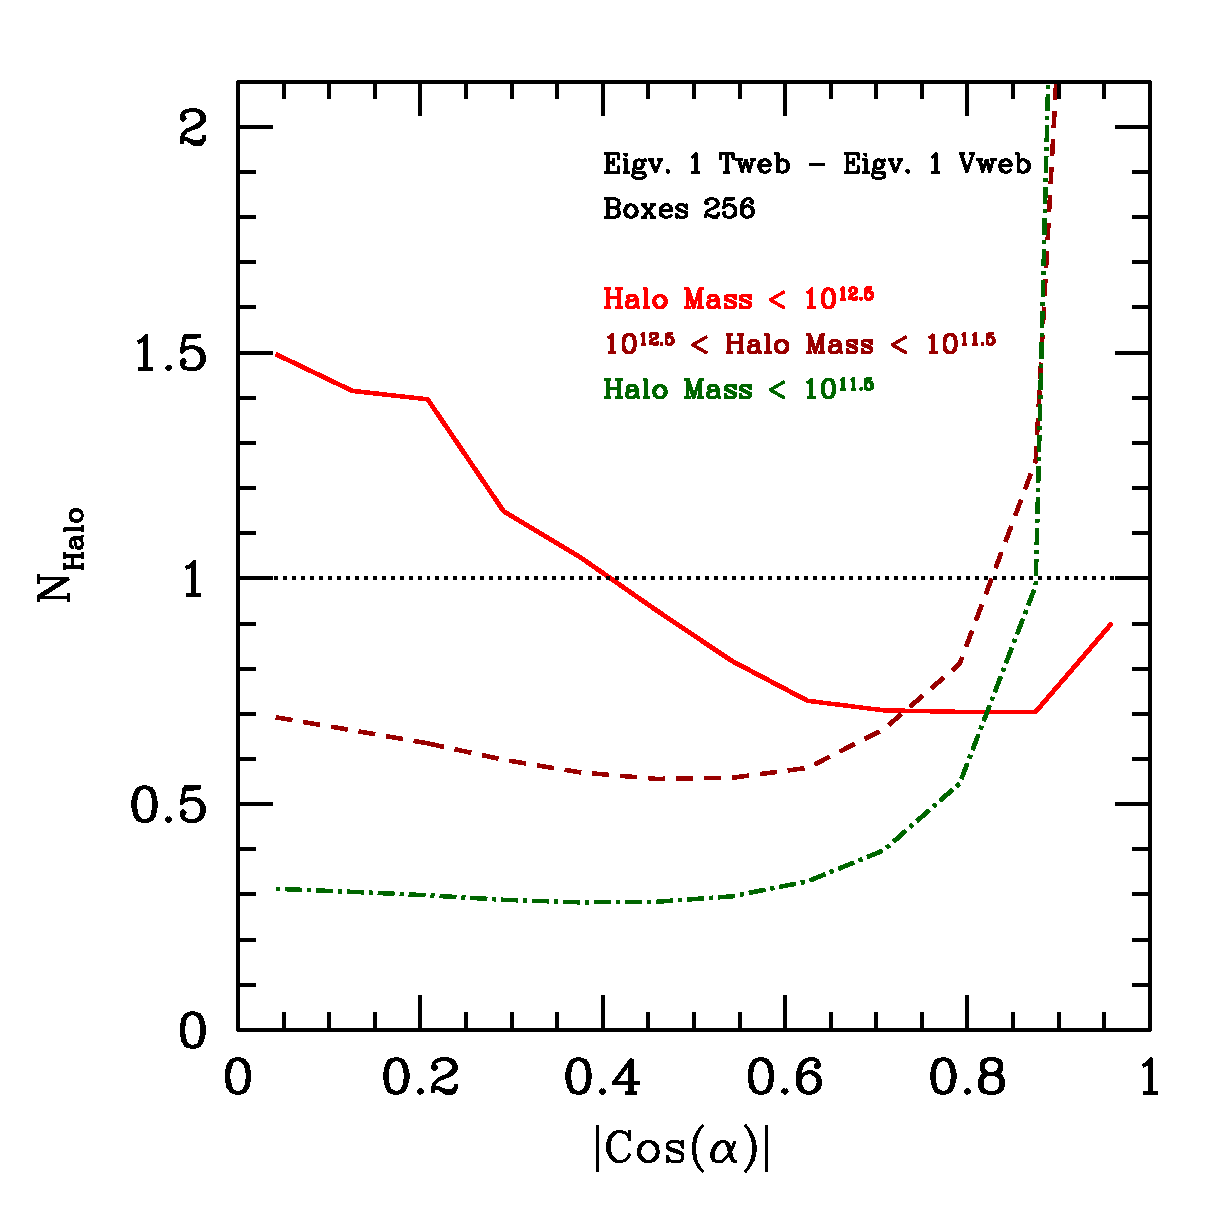
\includegraphics[width=0.30\textwidth]{../plot2/256/256_T1V1.ps}
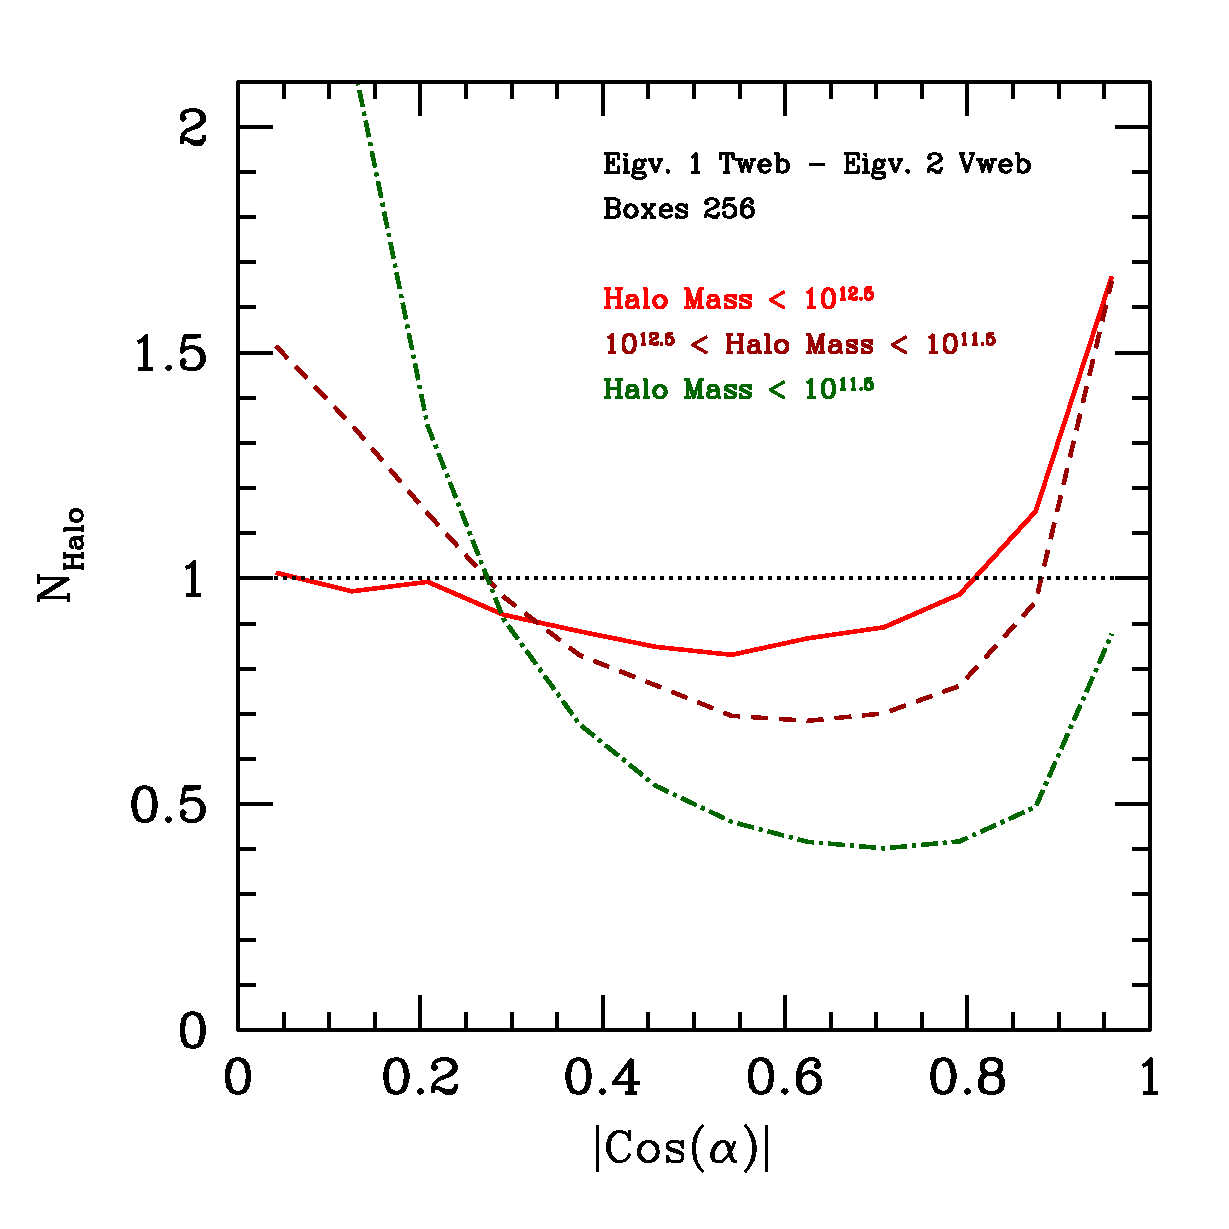
\includegraphics[width=0.30\textwidth]{../plot2/256/256_T1V2.ps}
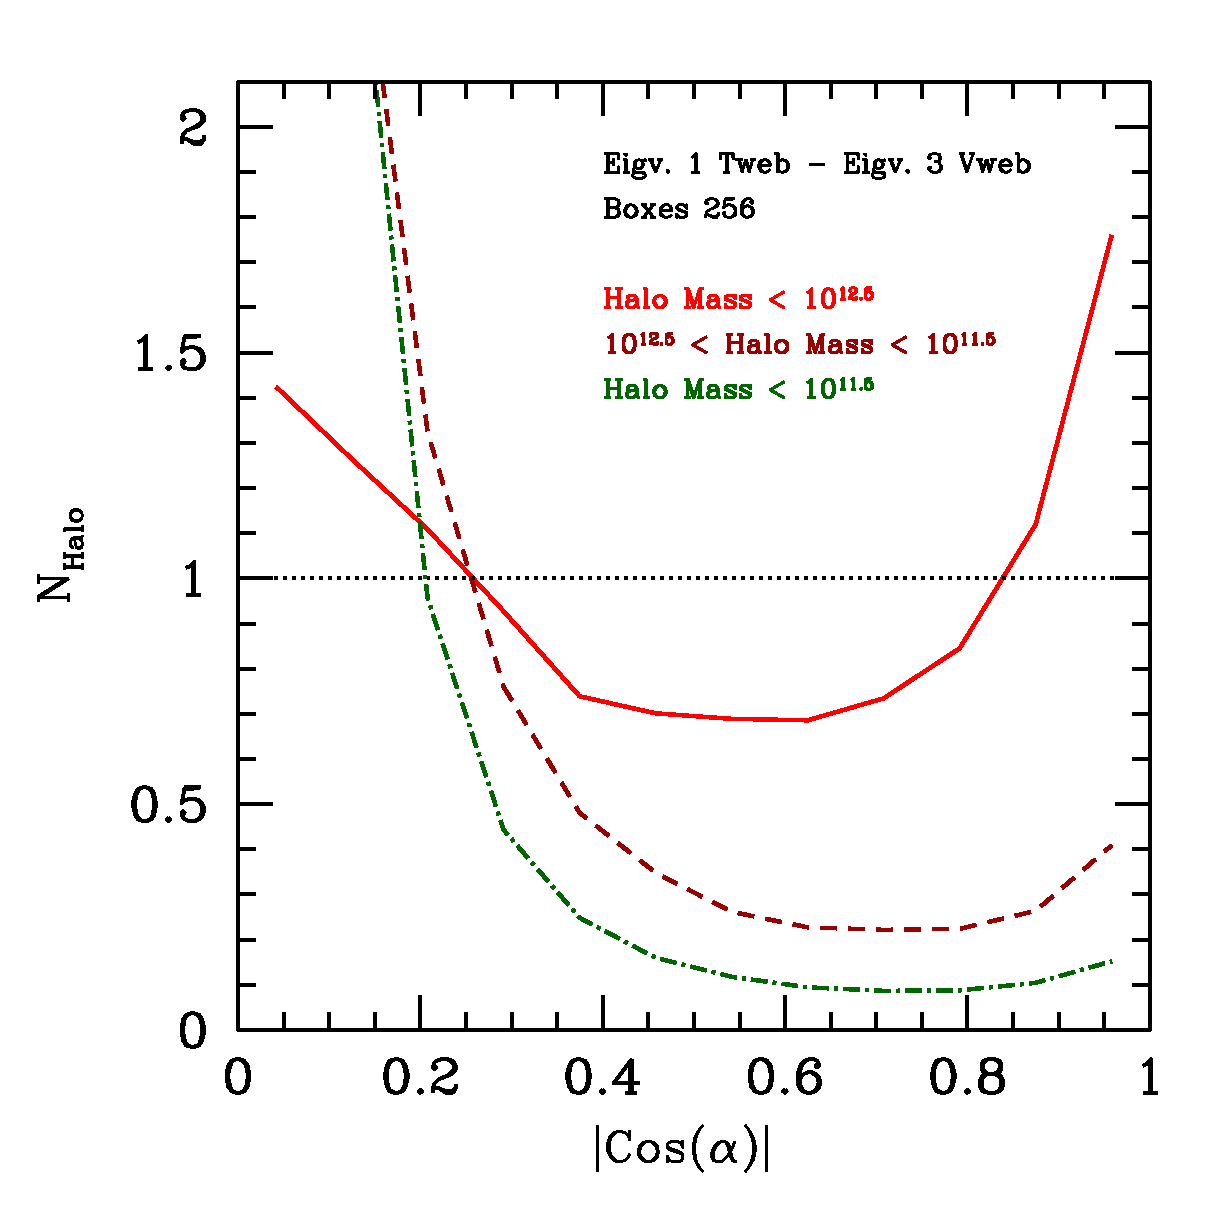
\includegraphics[width=0.30\textwidth]{../plot2/256/256_T1V3.ps}
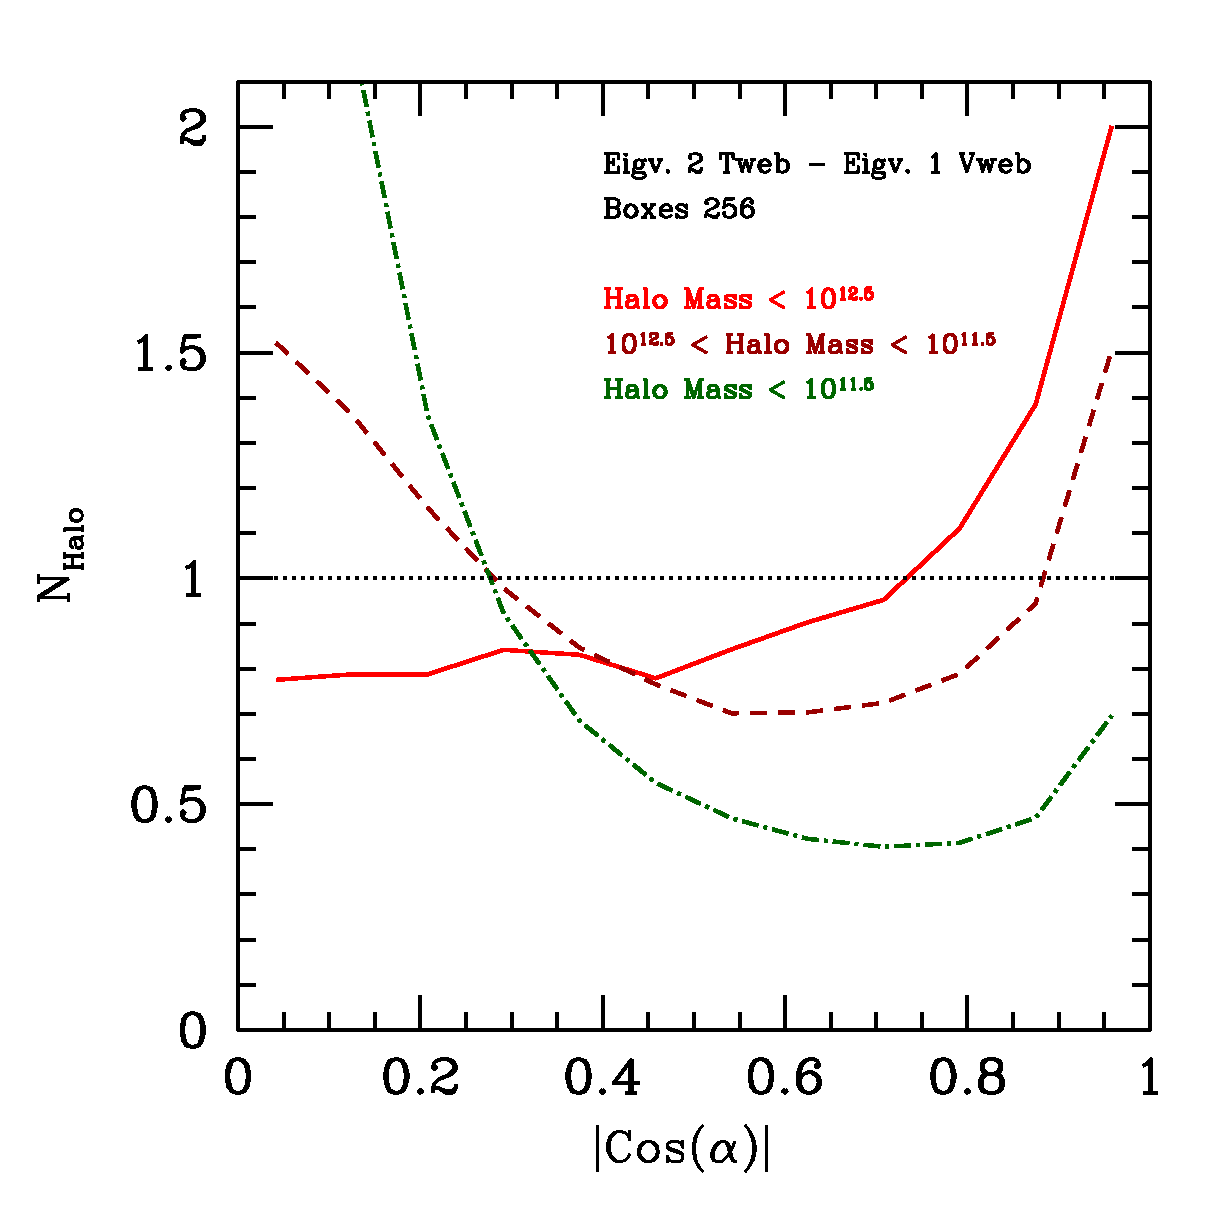
\includegraphics[width=0.30\textwidth]{../plot2/256/256_T2V1.ps}
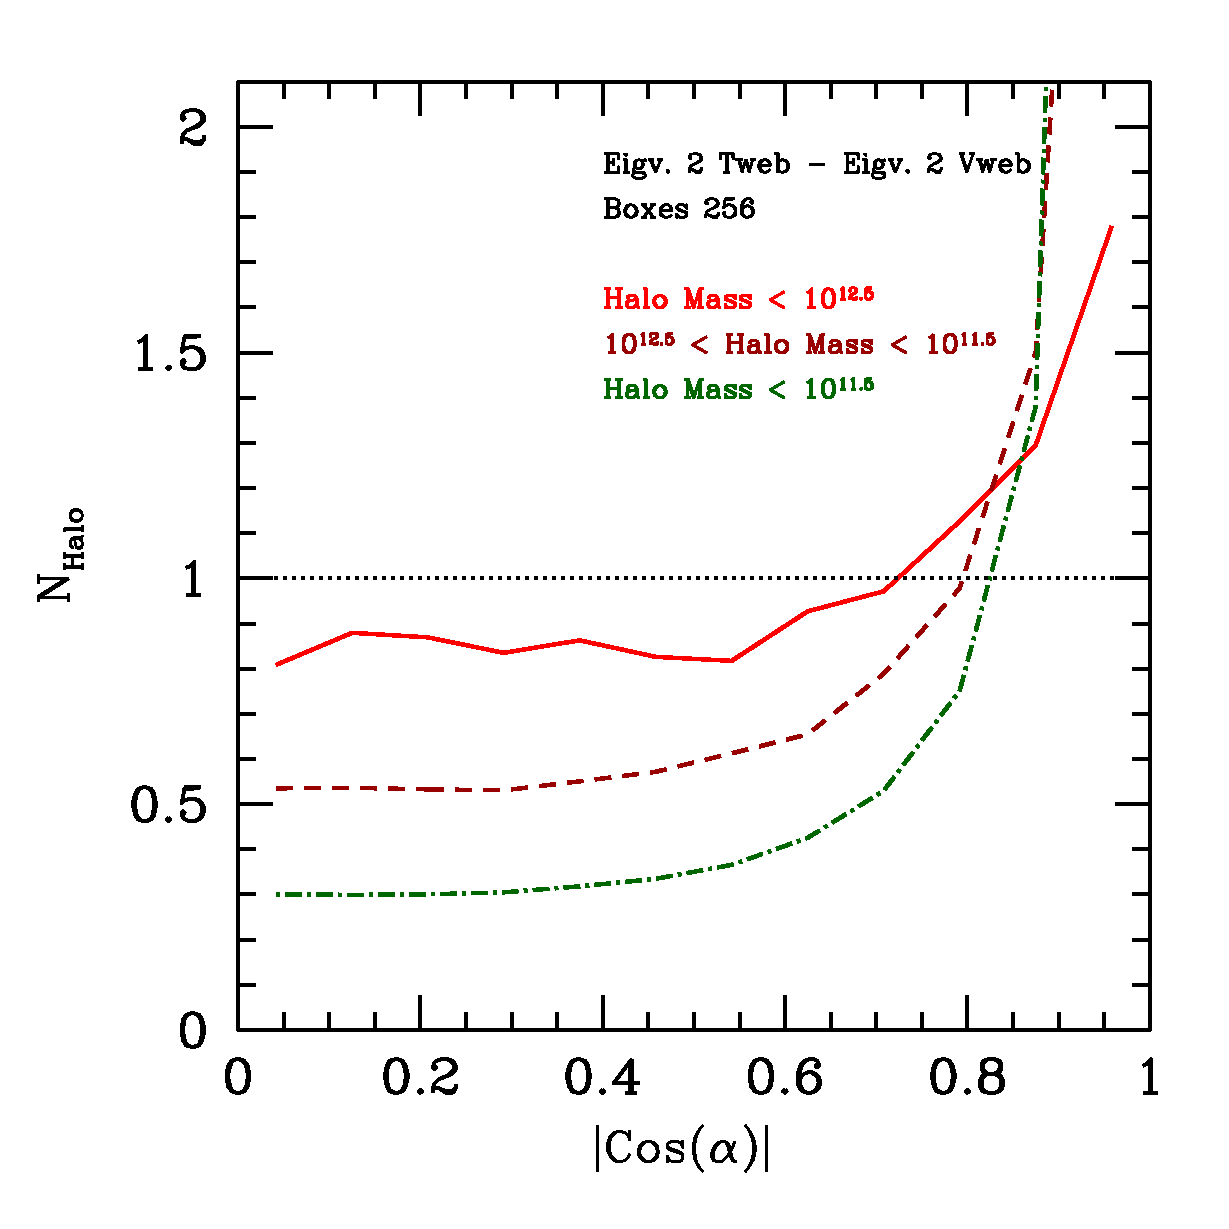
\includegraphics[width=0.30\textwidth]{../plot2/256/256_T2V2.ps}
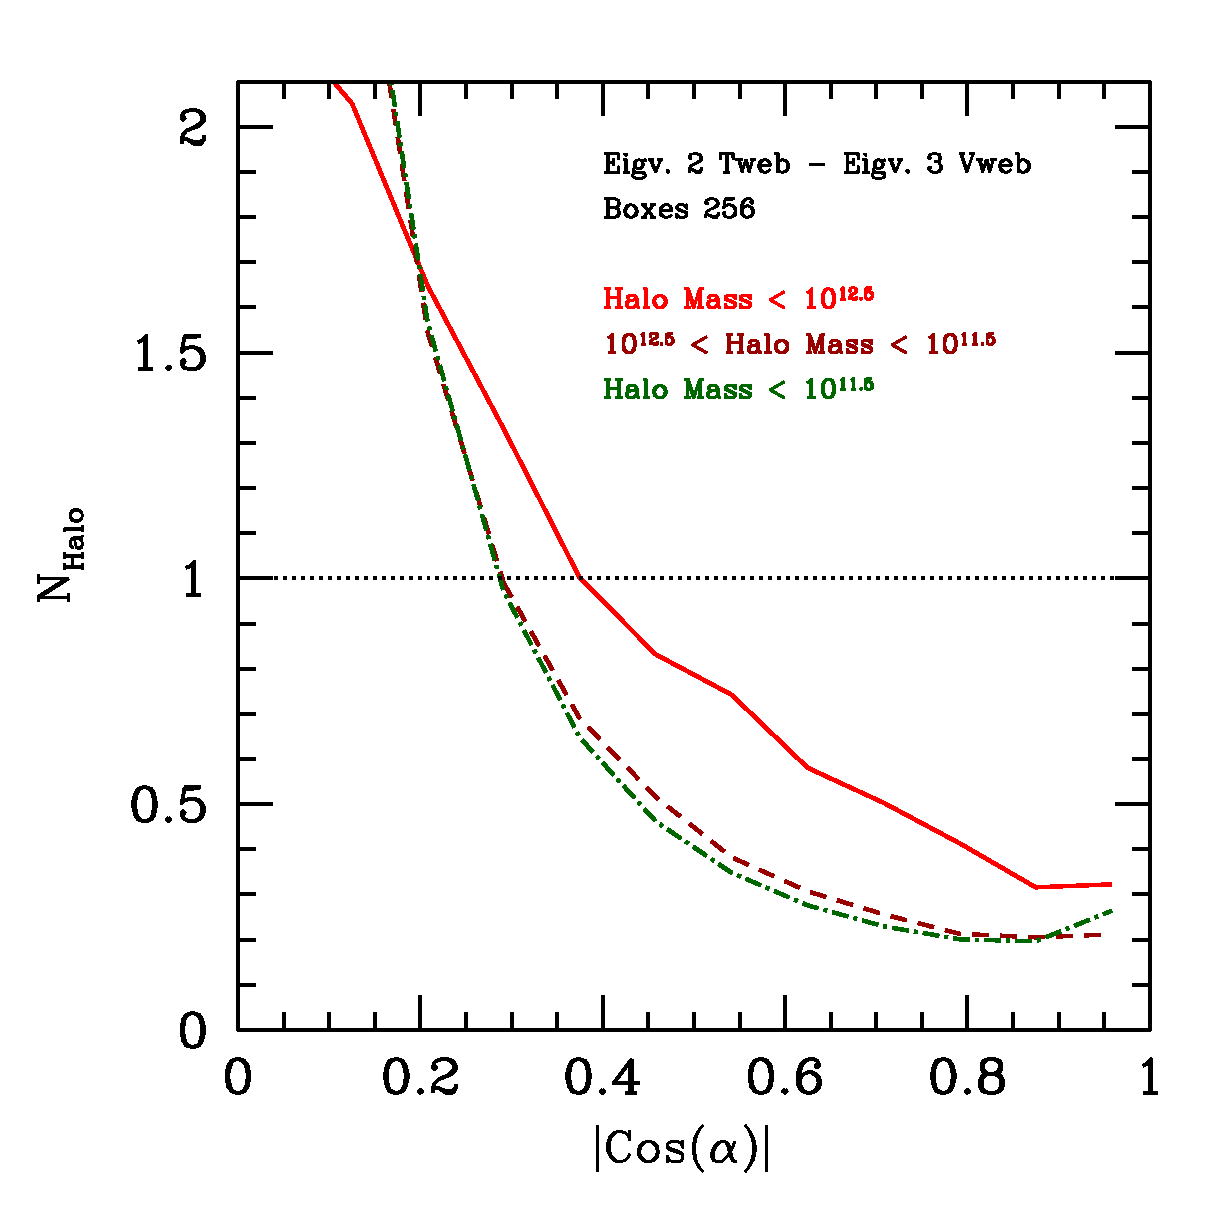
\includegraphics[width=0.30\textwidth]{../plot2/256/256_T2V3.ps}
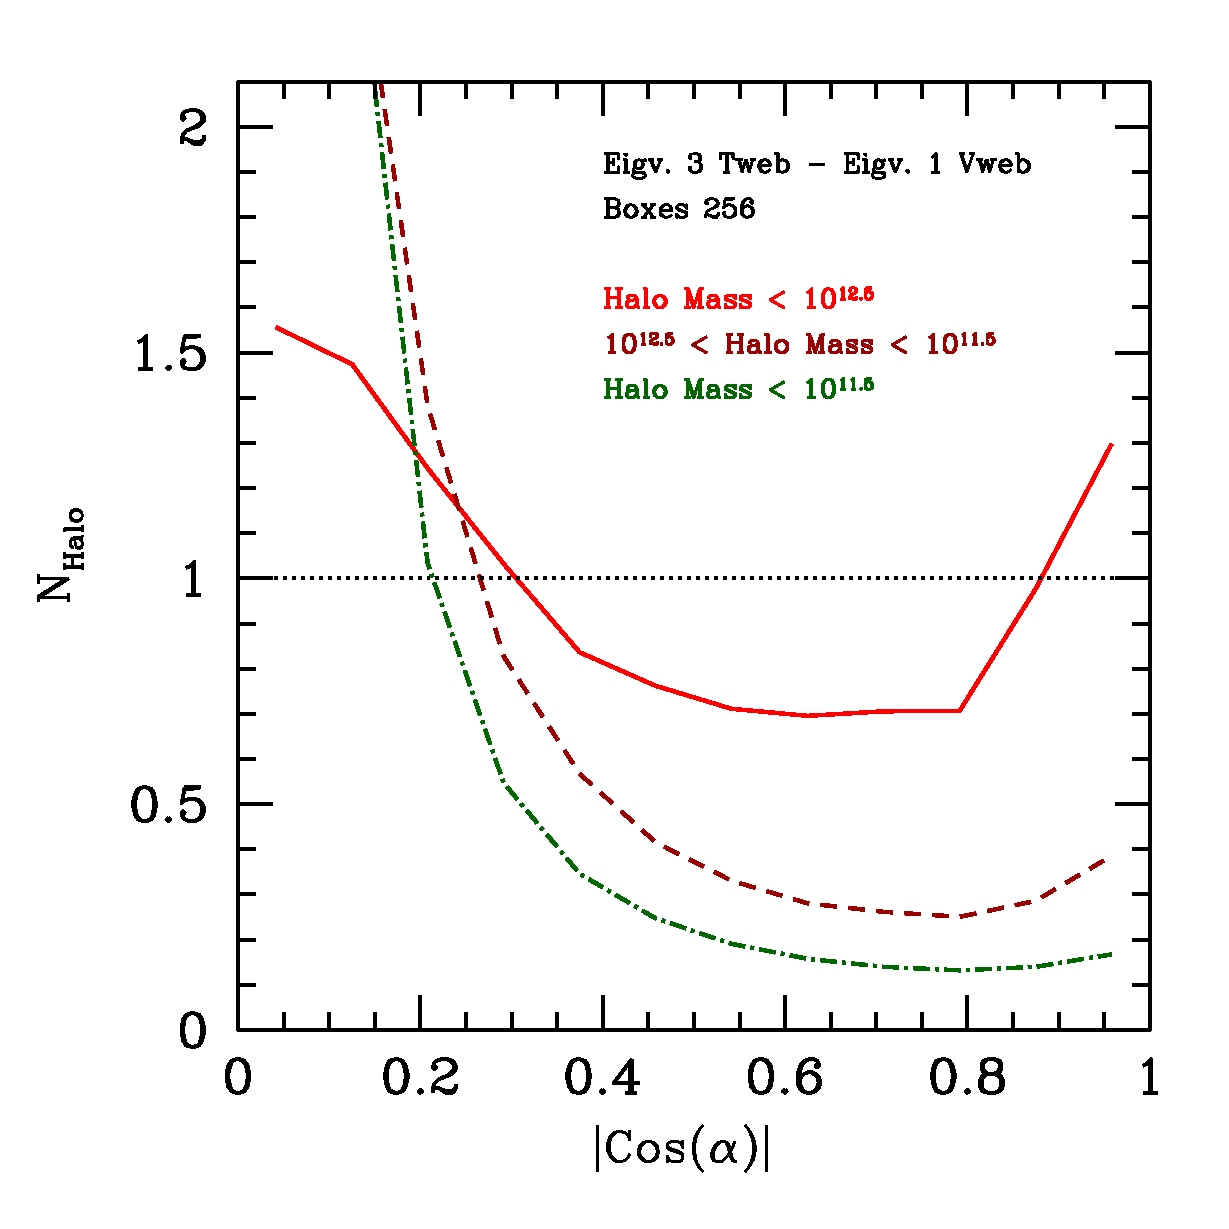
\includegraphics[width=0.30\textwidth]{../plot2/256/256_T3V1.ps}
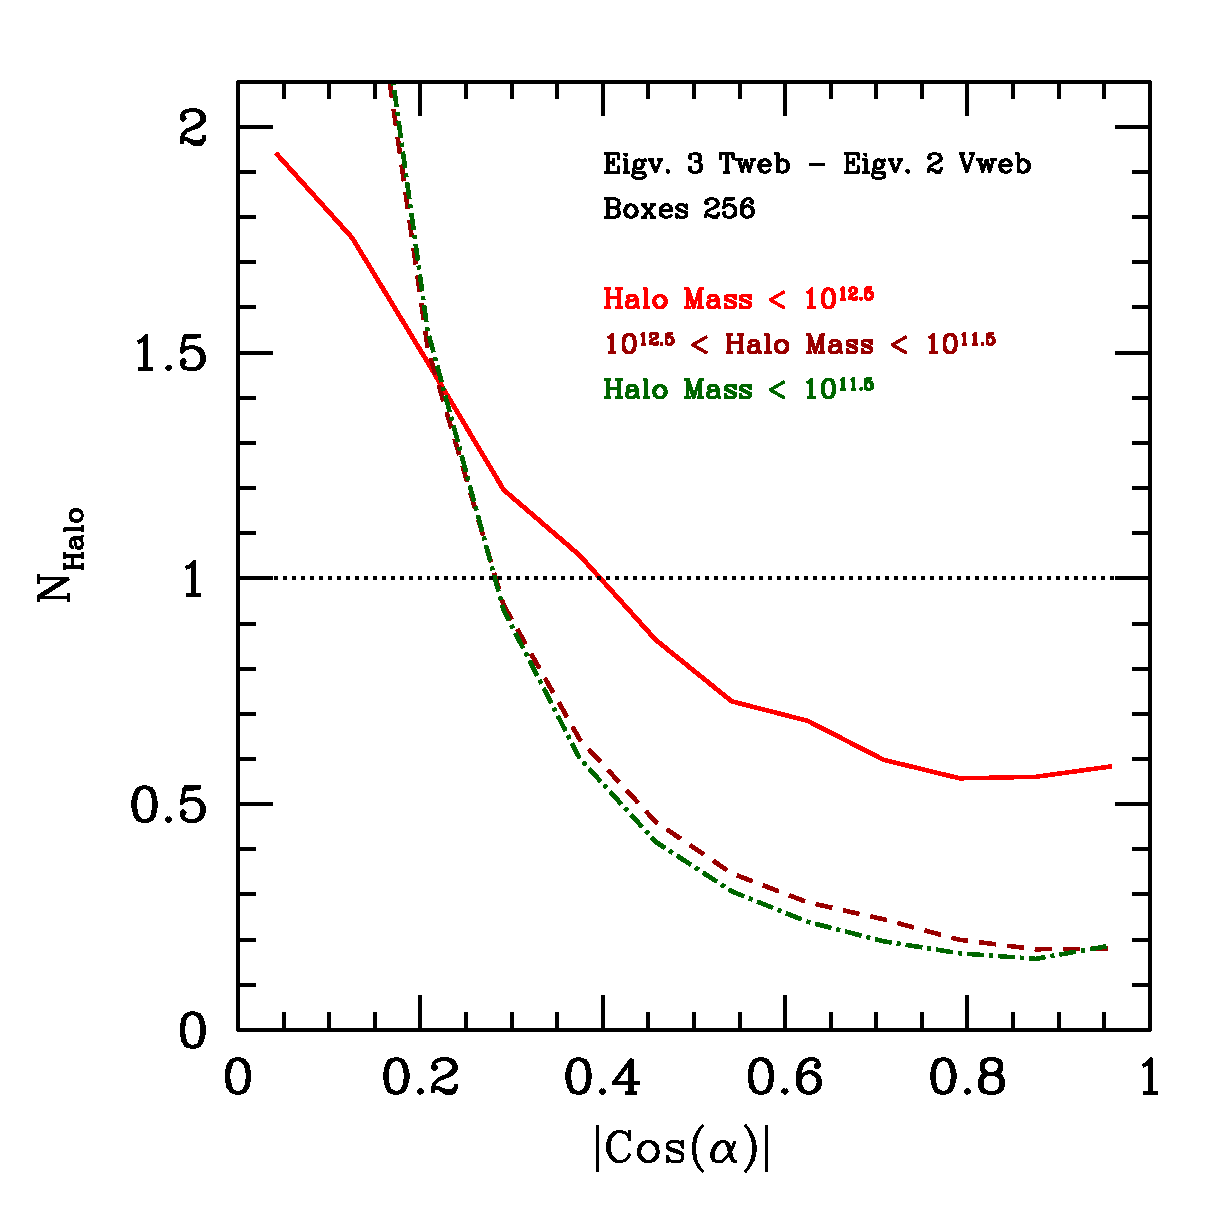
\includegraphics[width=0.30\textwidth]{../plot2/256/256_T3V2.ps}
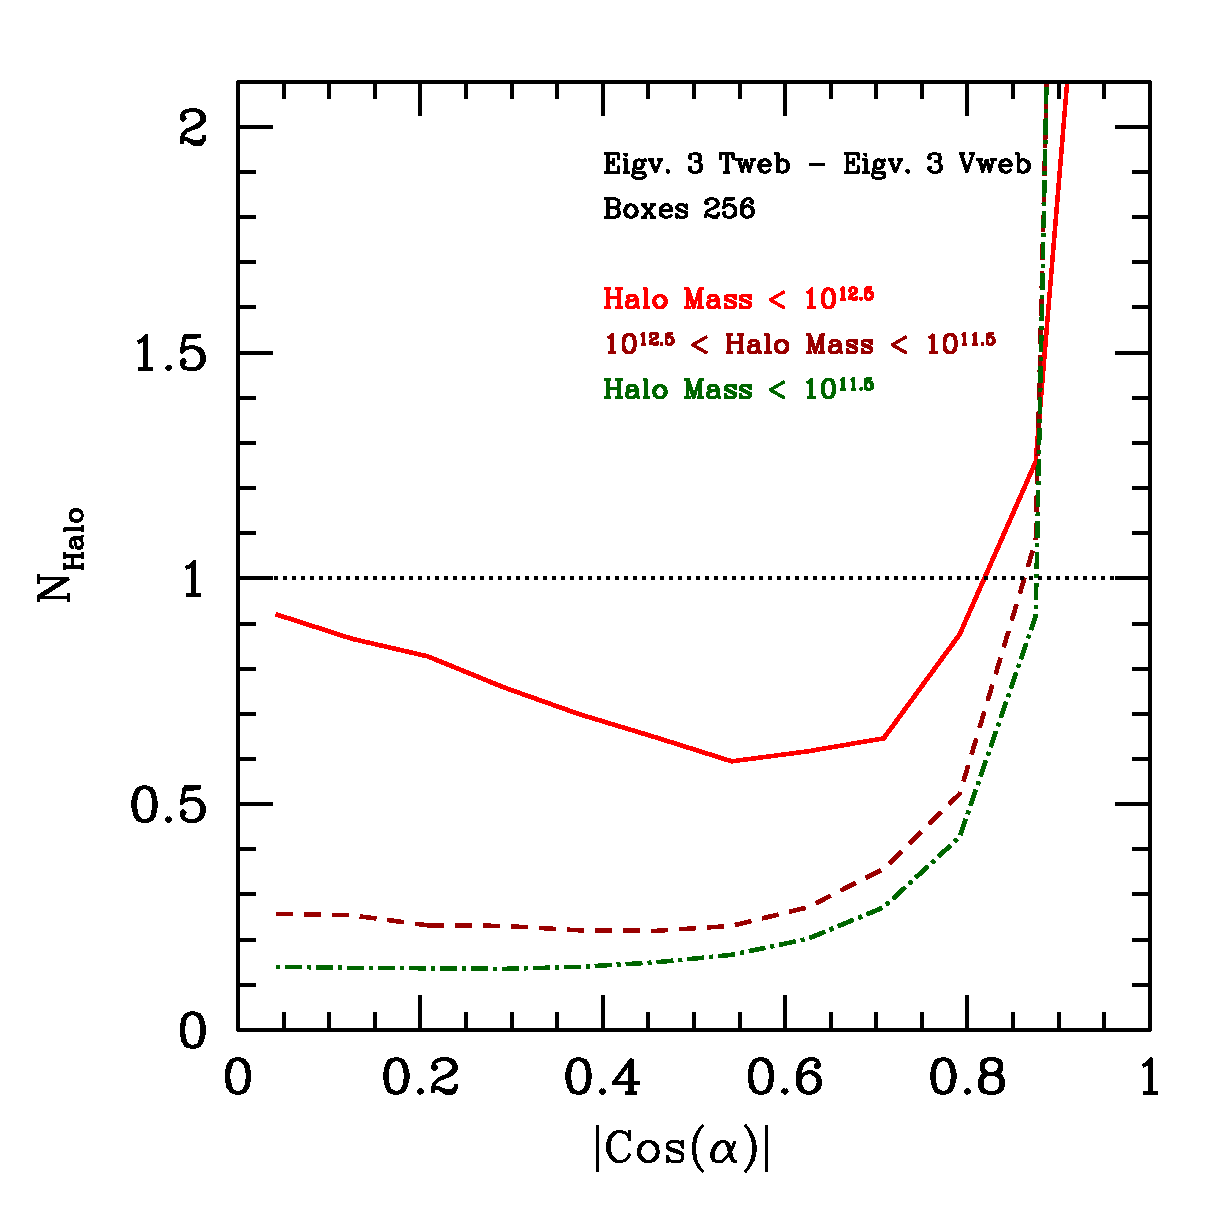
\includegraphics[width=0.30\textwidth]{../plot2/256/256_T3V3.ps}
\caption{Interweb alignment for $256^3$ grid resolution.}
\end{figure*}

\begin{figure*}
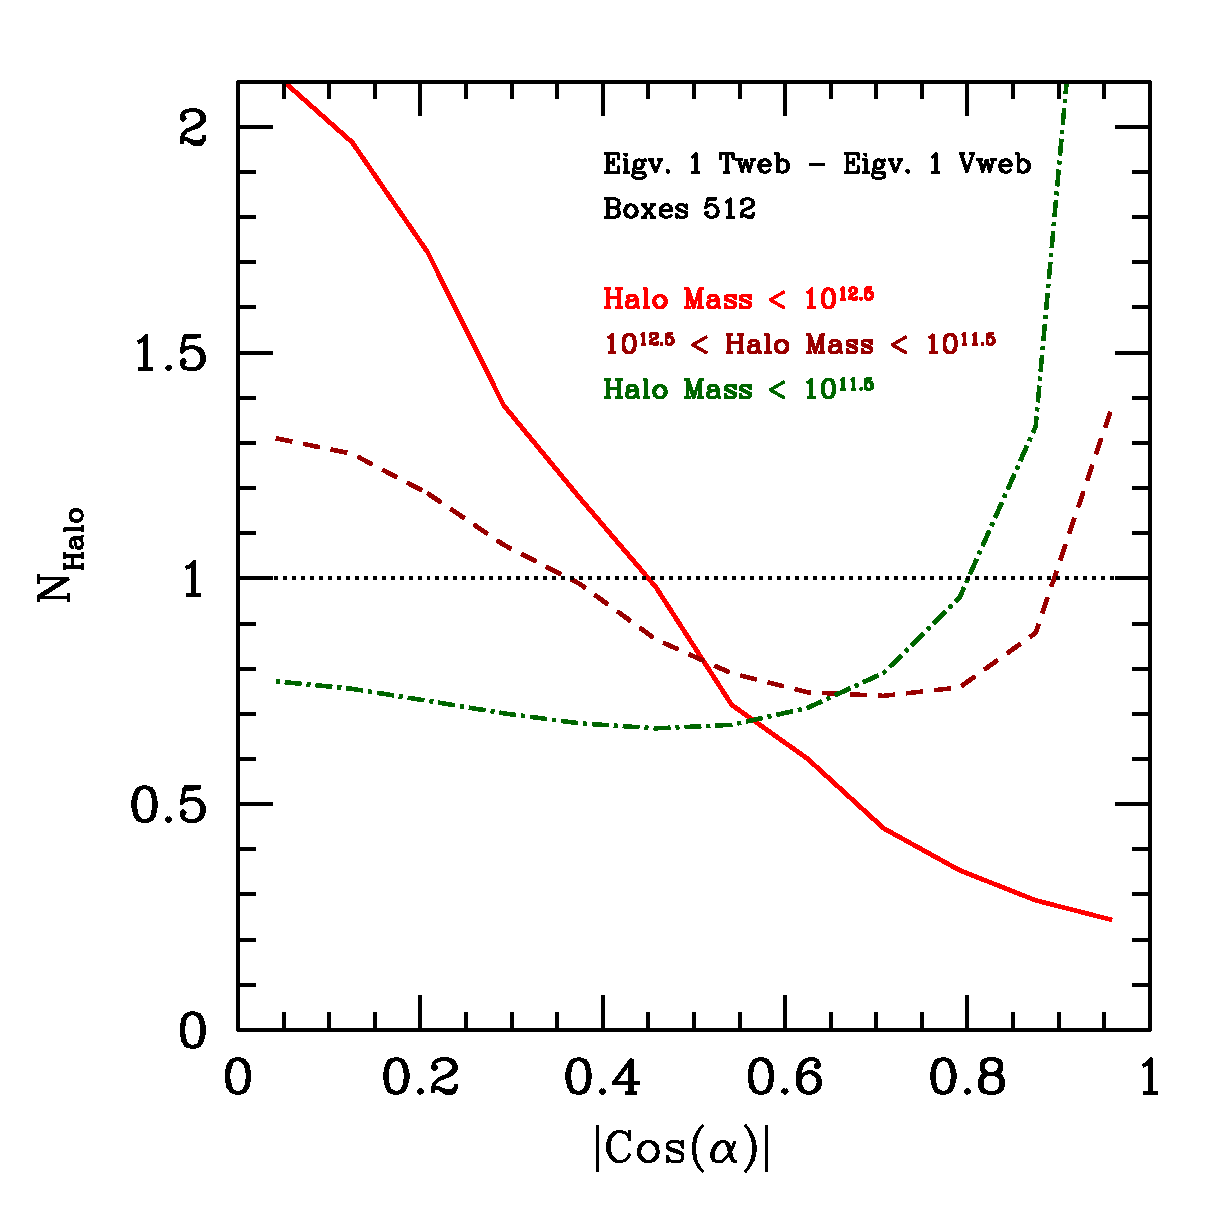
\includegraphics[width=0.30\textwidth]{../plot2/512/512_T1V1.ps}
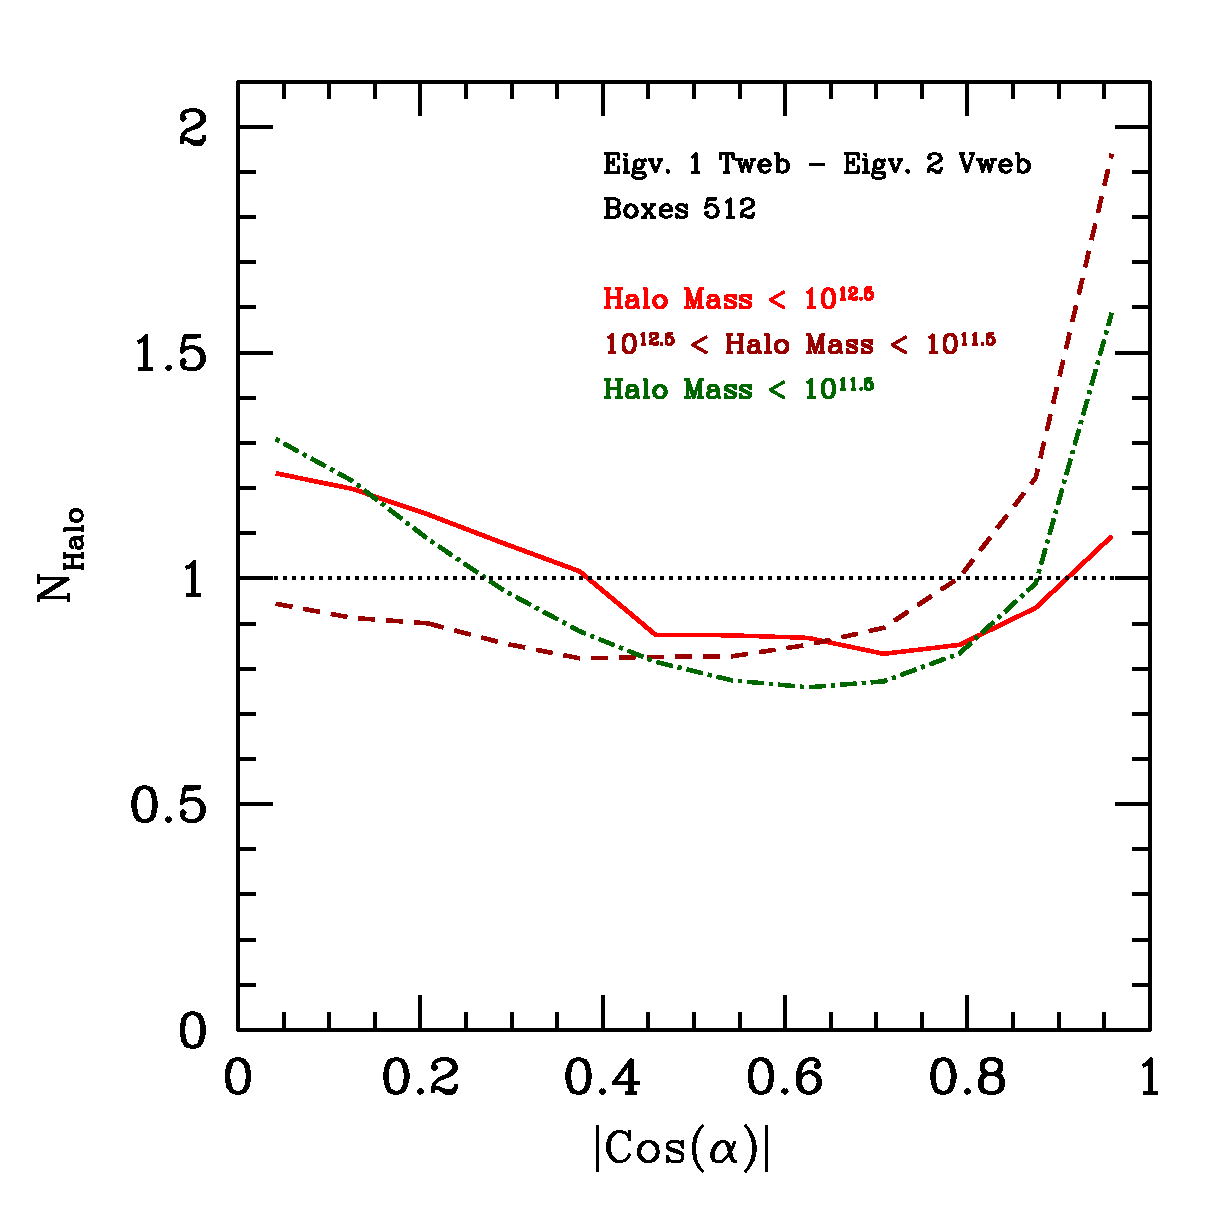
\includegraphics[width=0.30\textwidth]{../plot2/512/512_T1V2.ps}
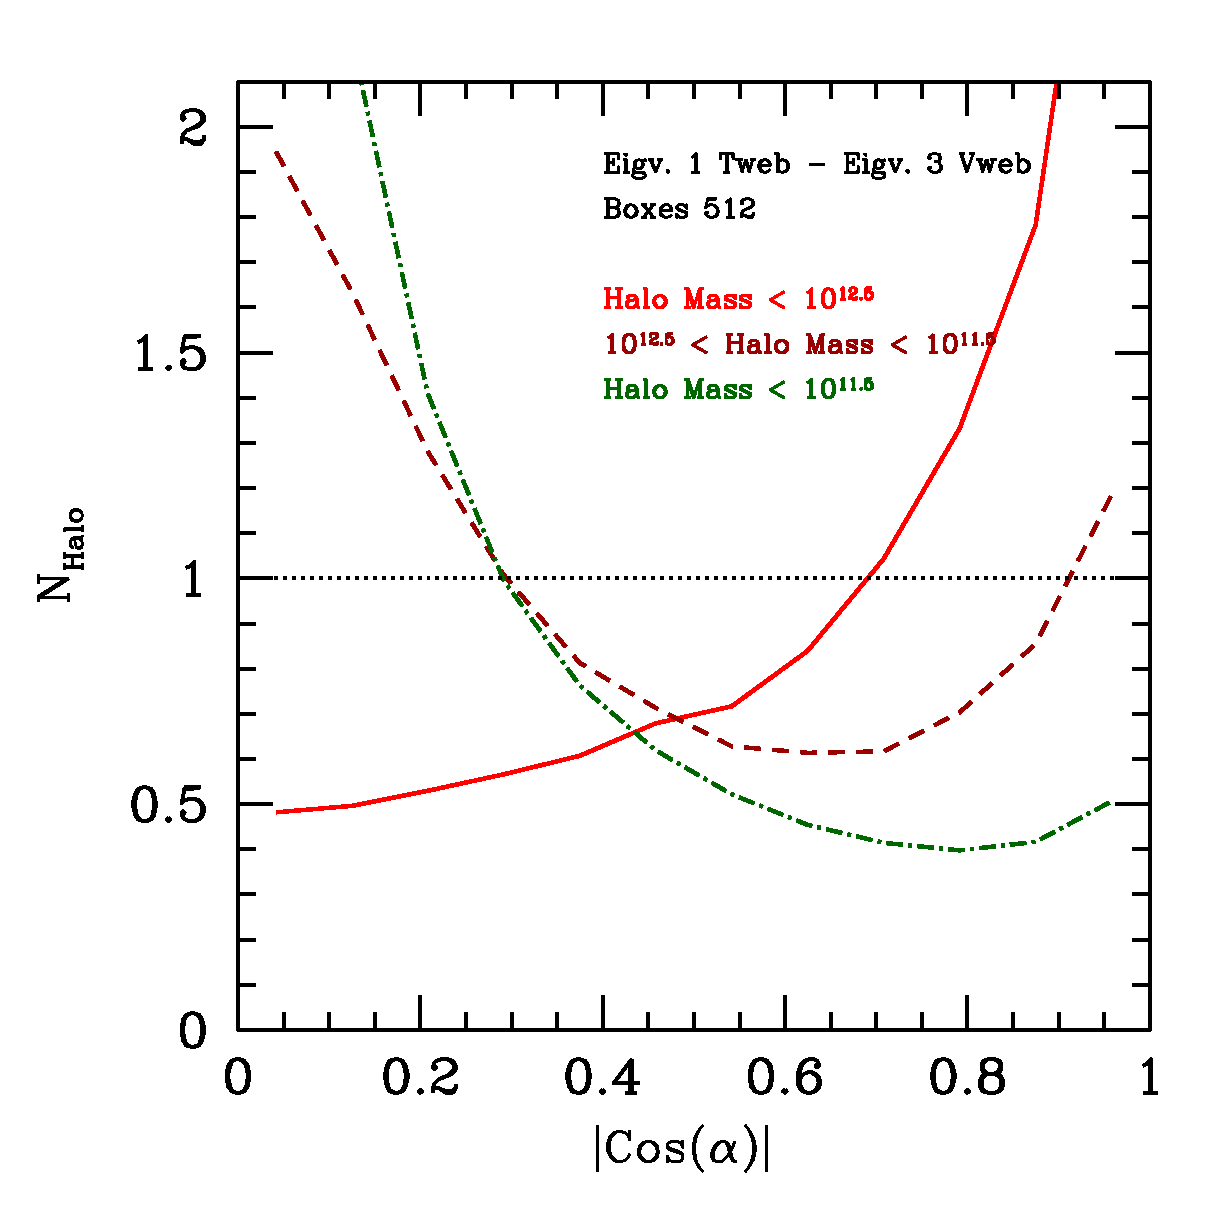
\includegraphics[width=0.30\textwidth]{../plot2/512/512_T1V3.ps}
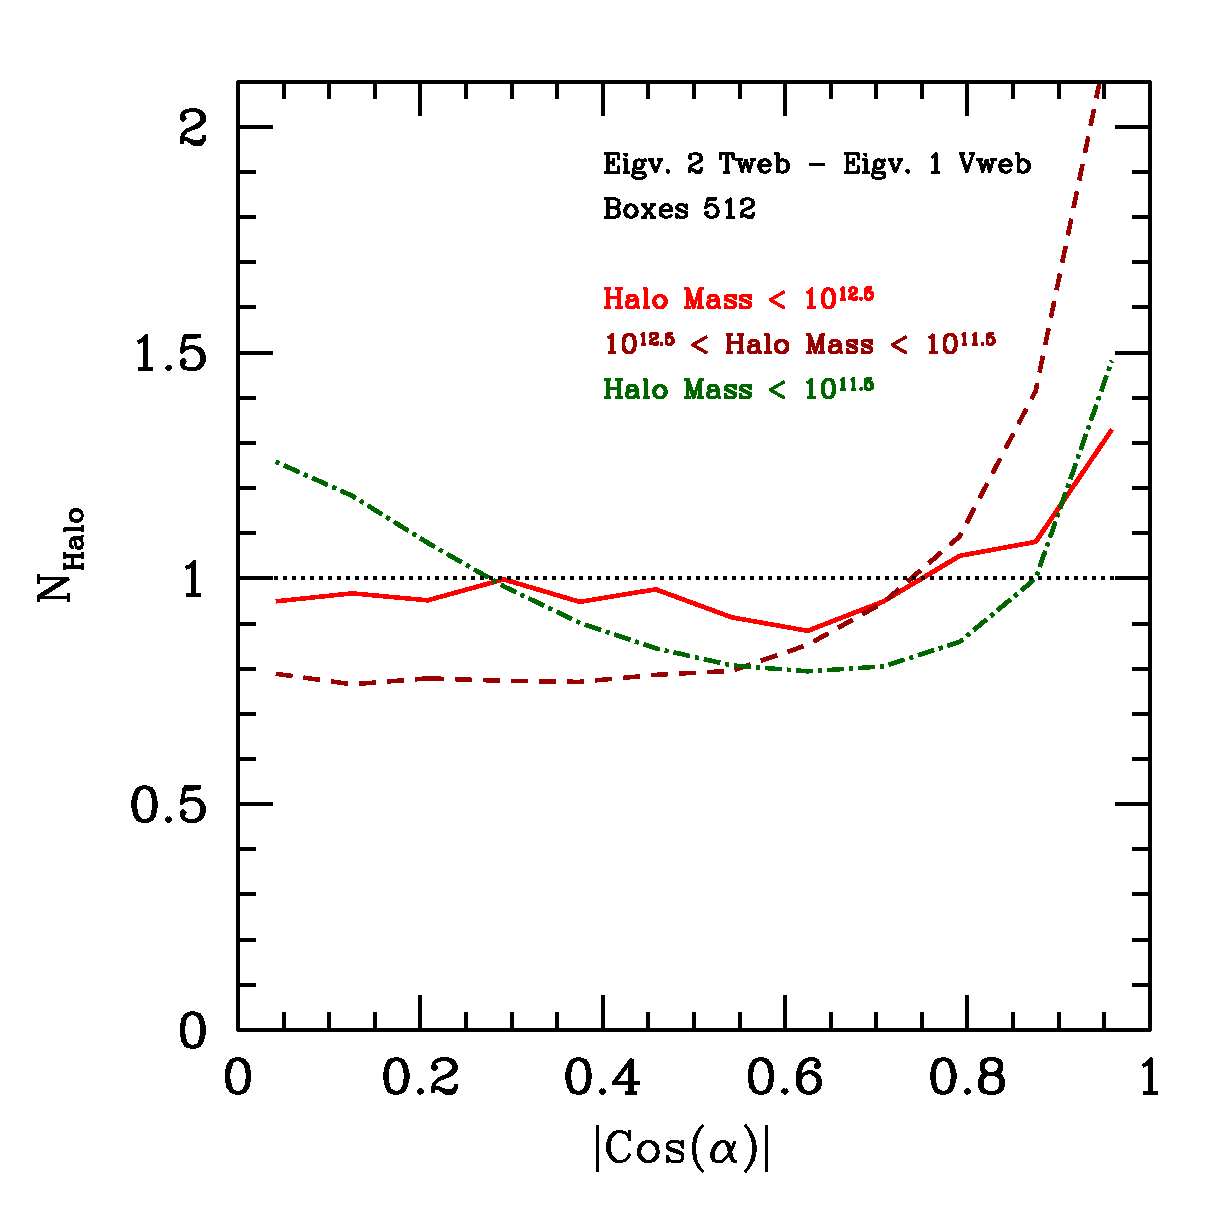
\includegraphics[width=0.30\textwidth]{../plot2/512/512_T2V1.ps}
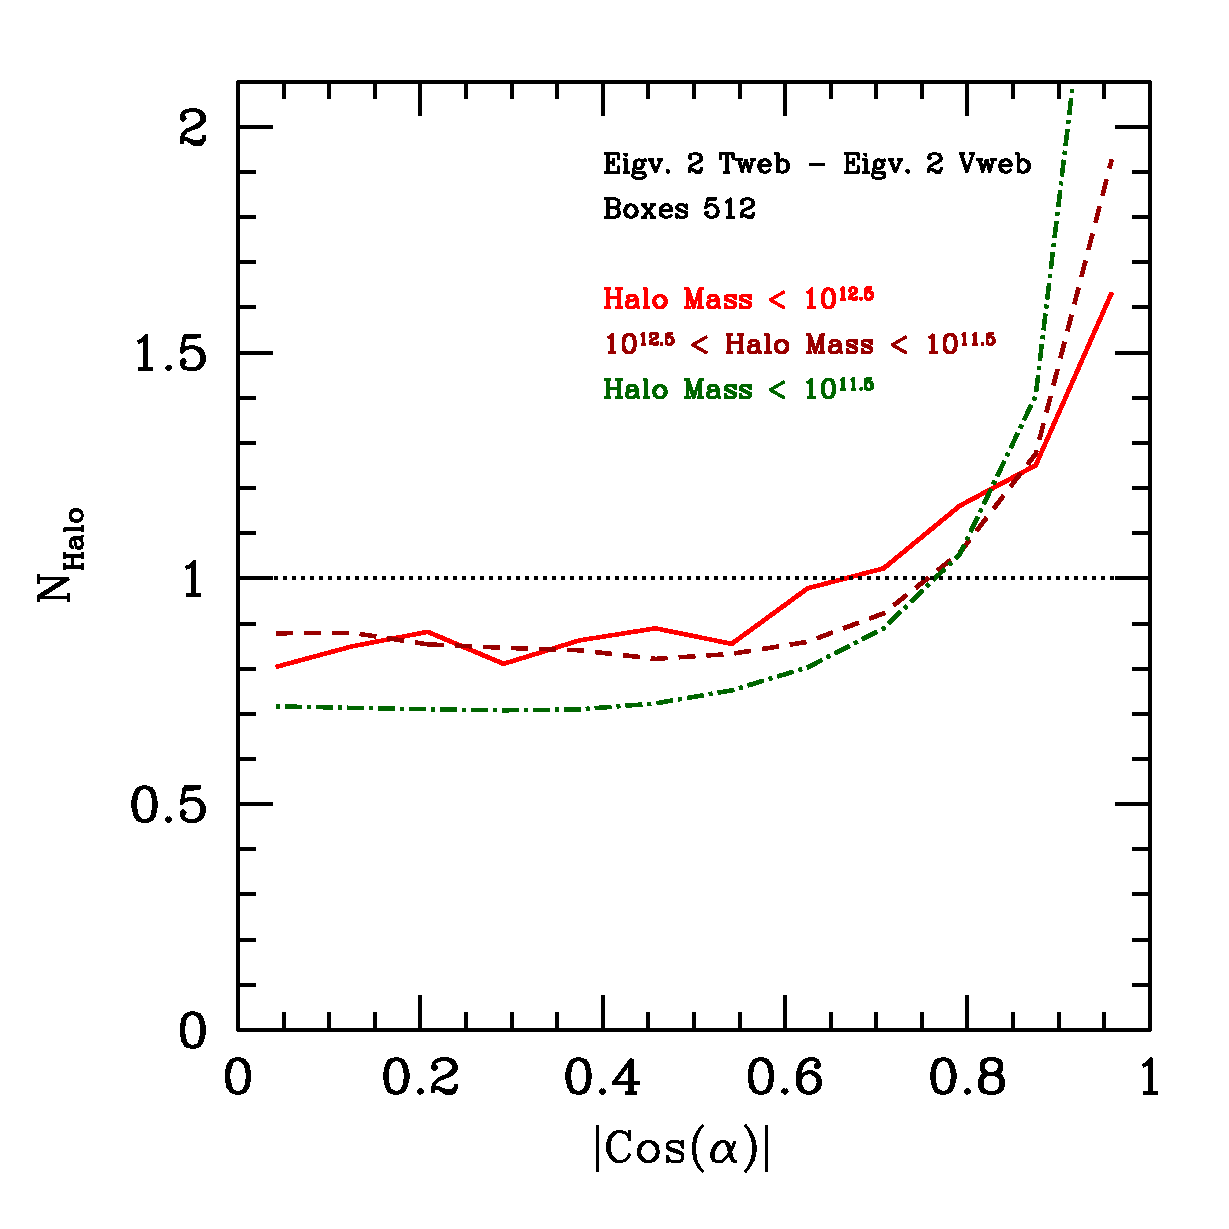
\includegraphics[width=0.30\textwidth]{../plot2/512/512_T2V2.ps}
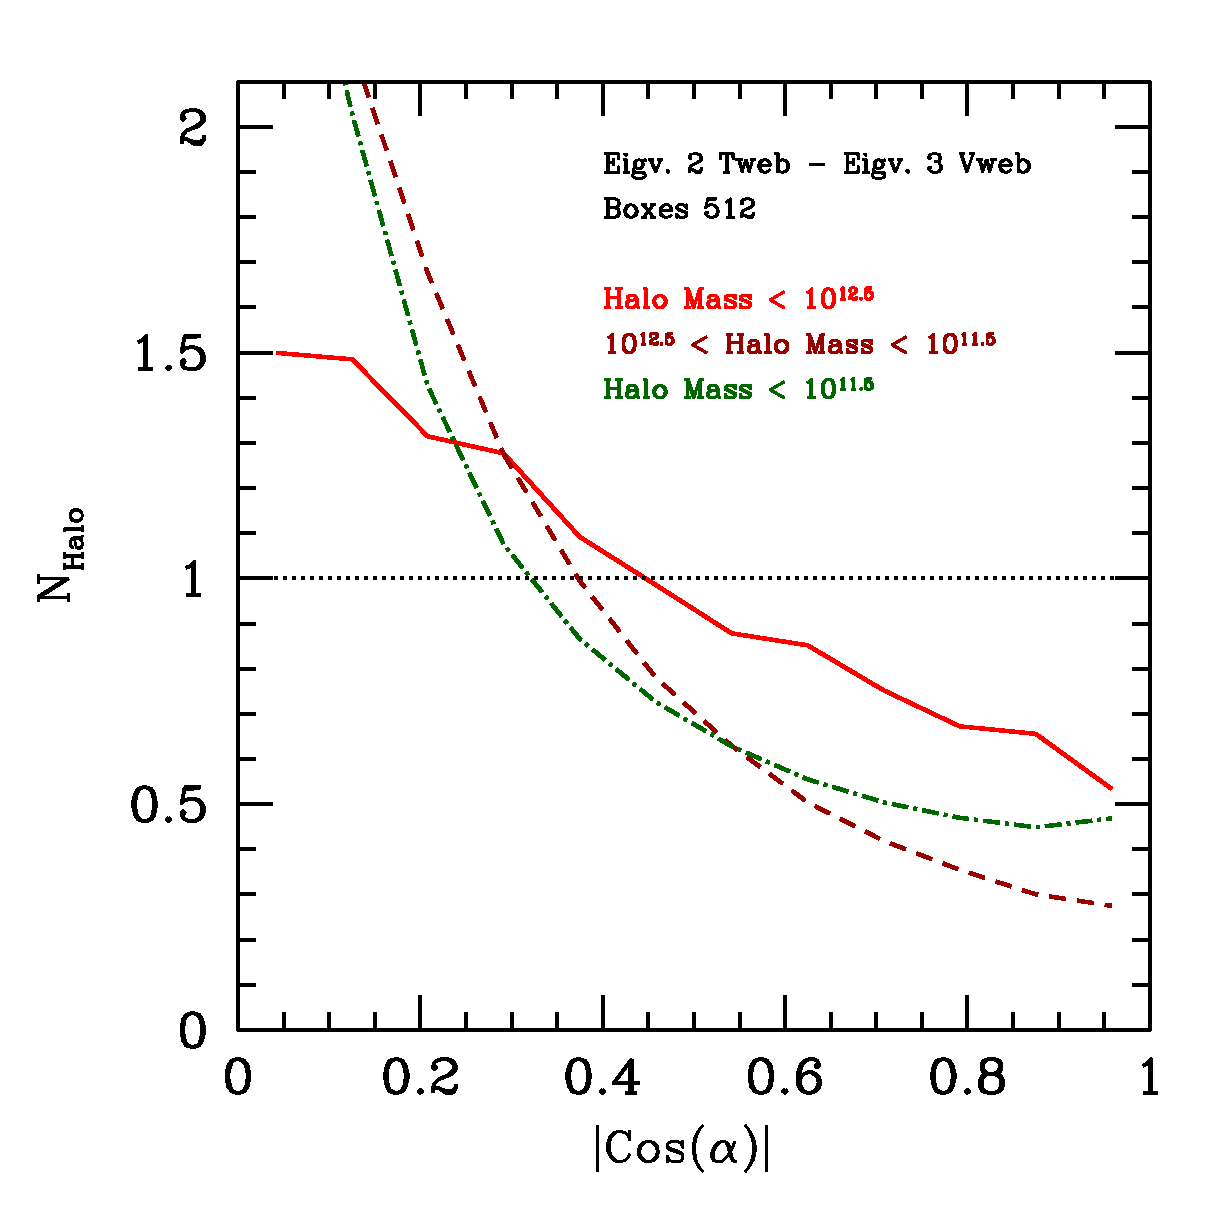
\includegraphics[width=0.30\textwidth]{../plot2/512/512_T2V3.ps}
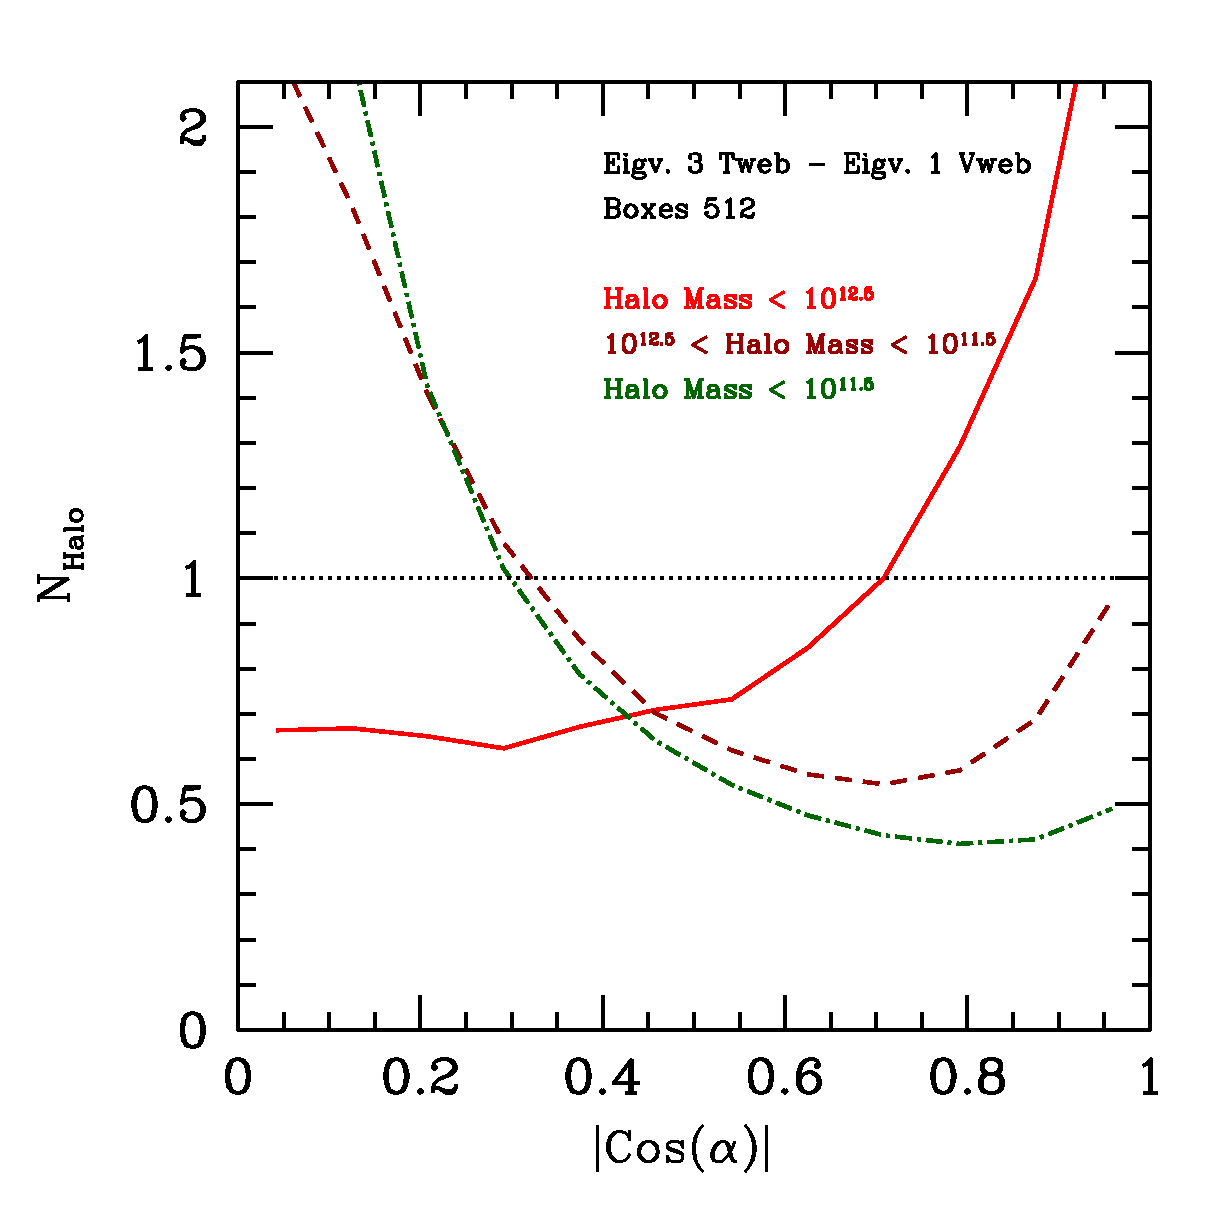
\includegraphics[width=0.30\textwidth]{../plot2/512/512_T3V1.ps}
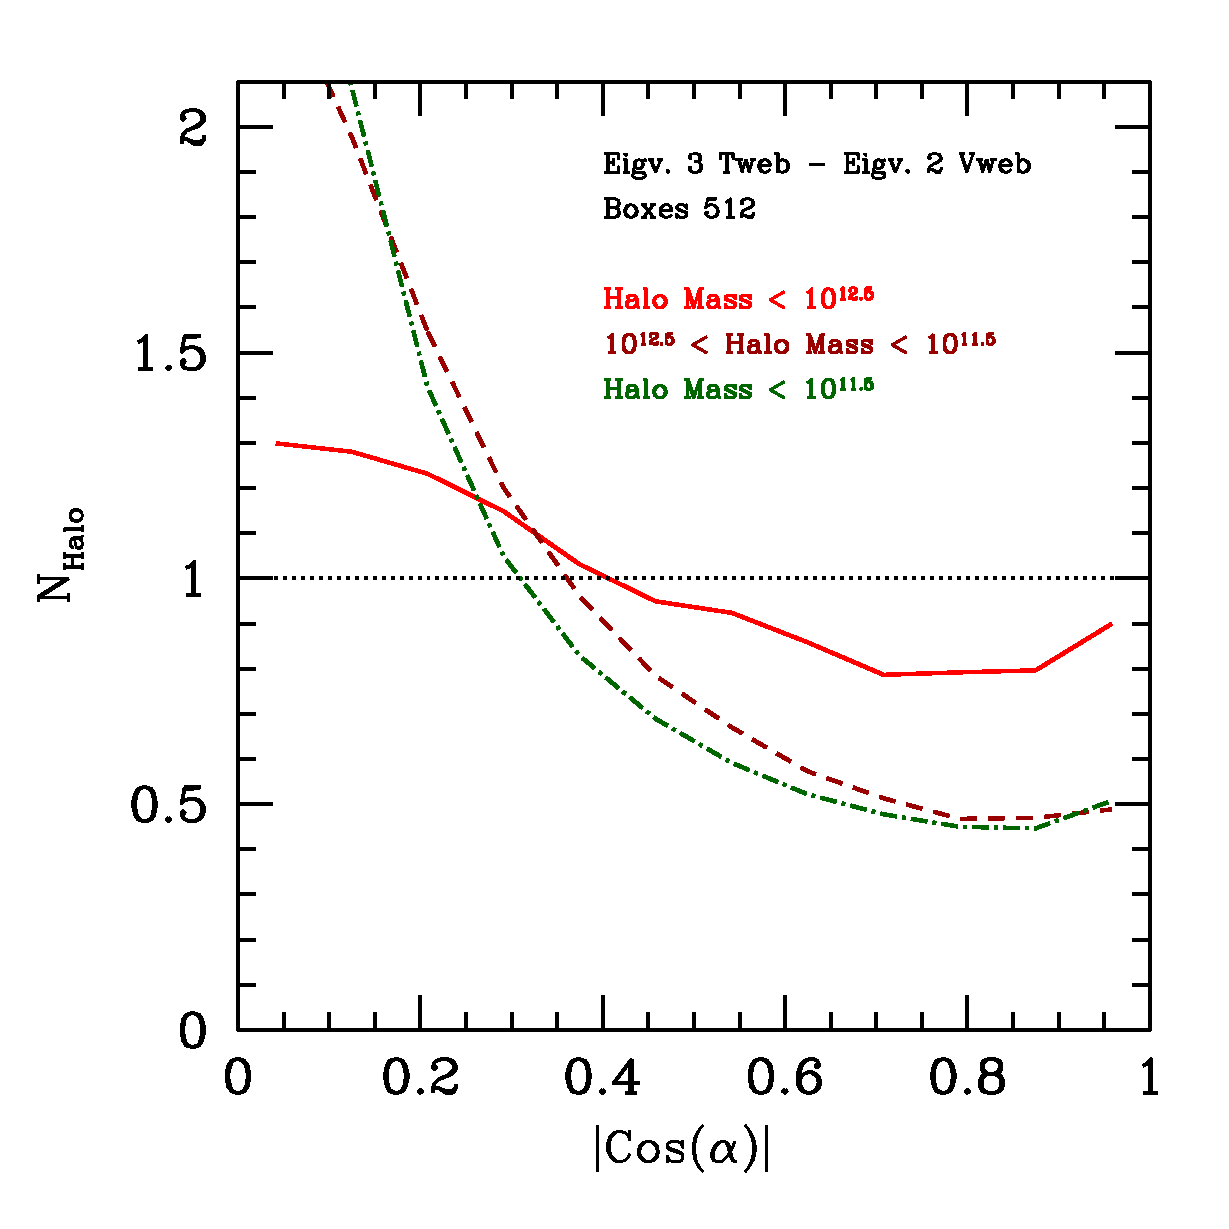
\includegraphics[width=0.30\textwidth]{../plot2/512/512_T3V2.ps}
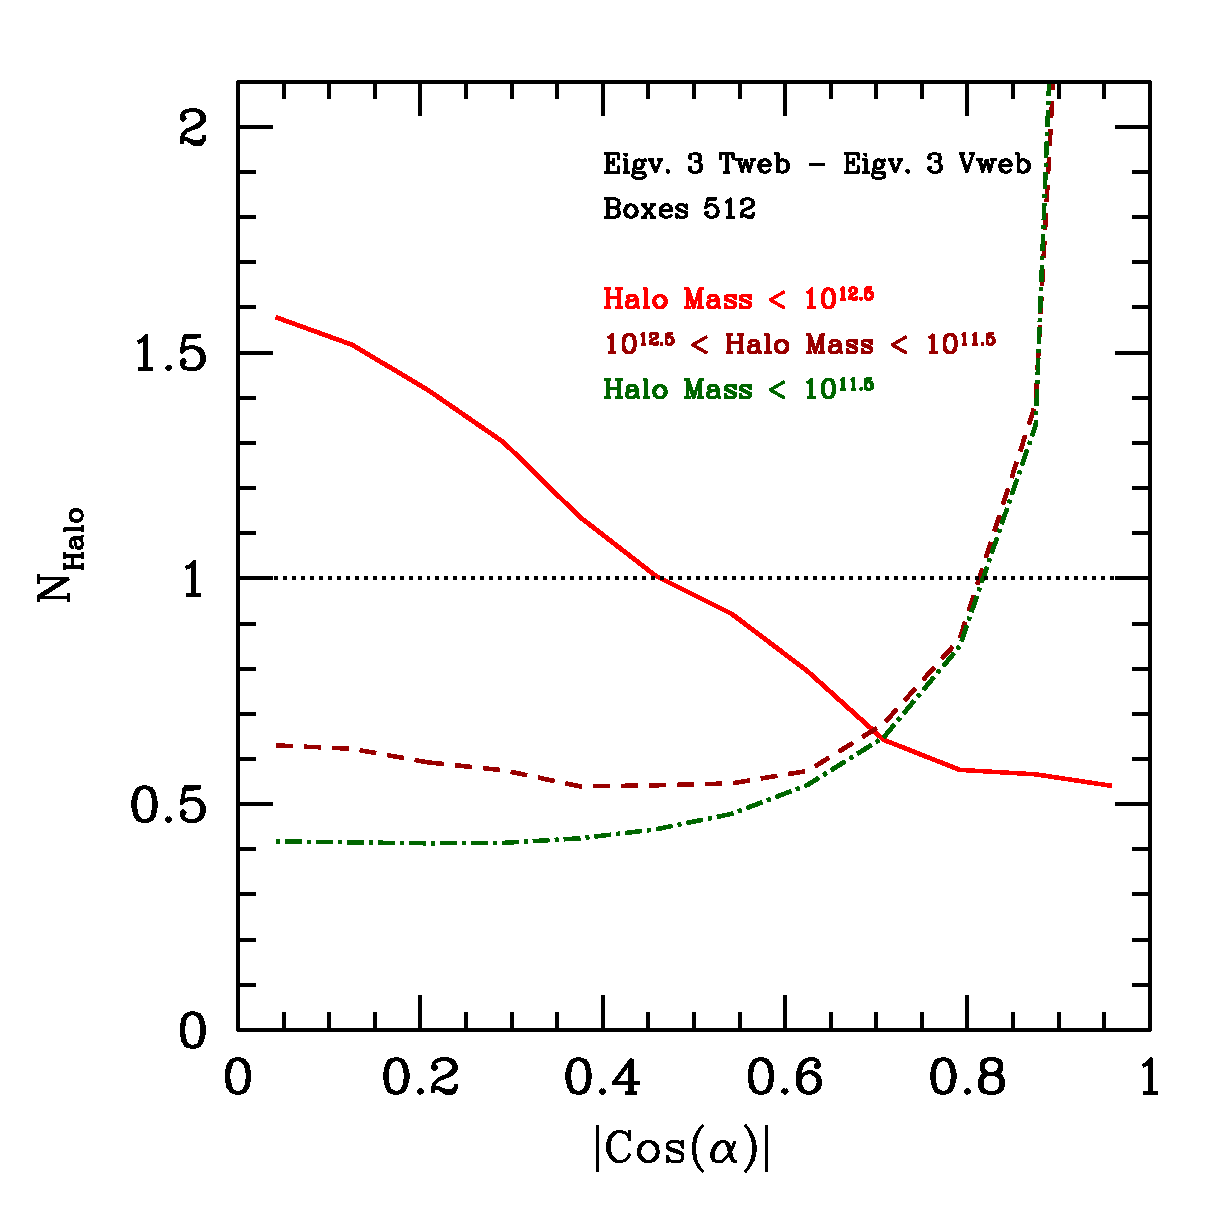
\includegraphics[width=0.30\textwidth]{../plot2/512/512_T3V3.ps}
\caption{Interweb alignment for $512^3$ grid resolution.}
\end{figure*}

\begin{figure*}
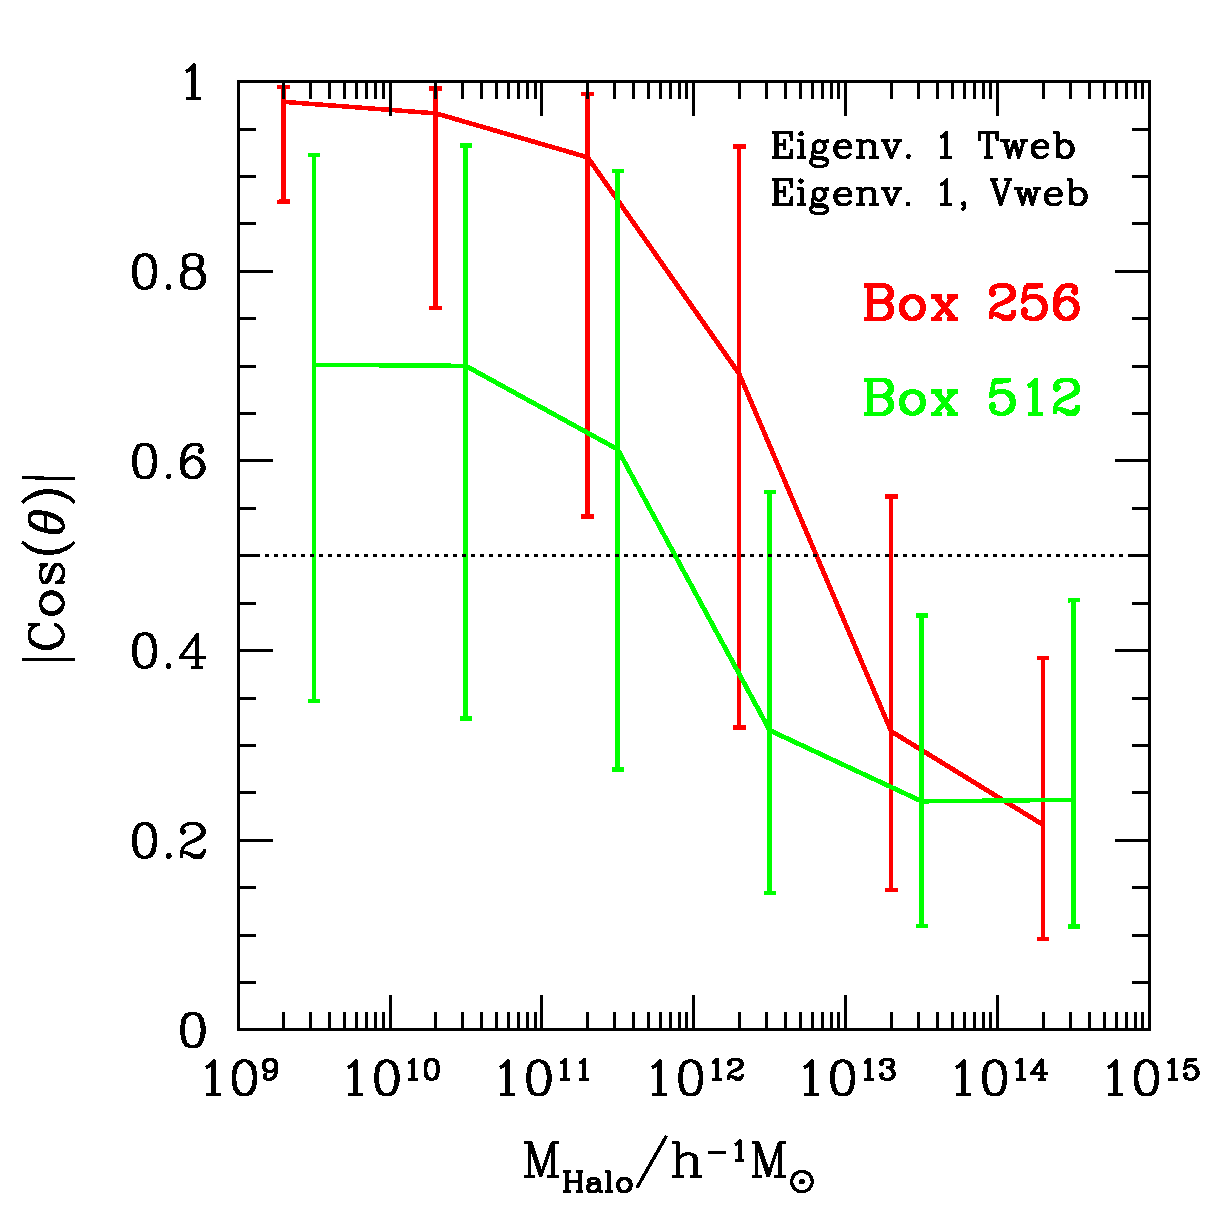
\includegraphics[width=0.30\textwidth]{../plot2/Mass/Web.ps}
\caption{Median of the interweb alignment for the two grid resolution.}
\end{figure*}

\subsection{Shape Alignment}

\begin{figure*}
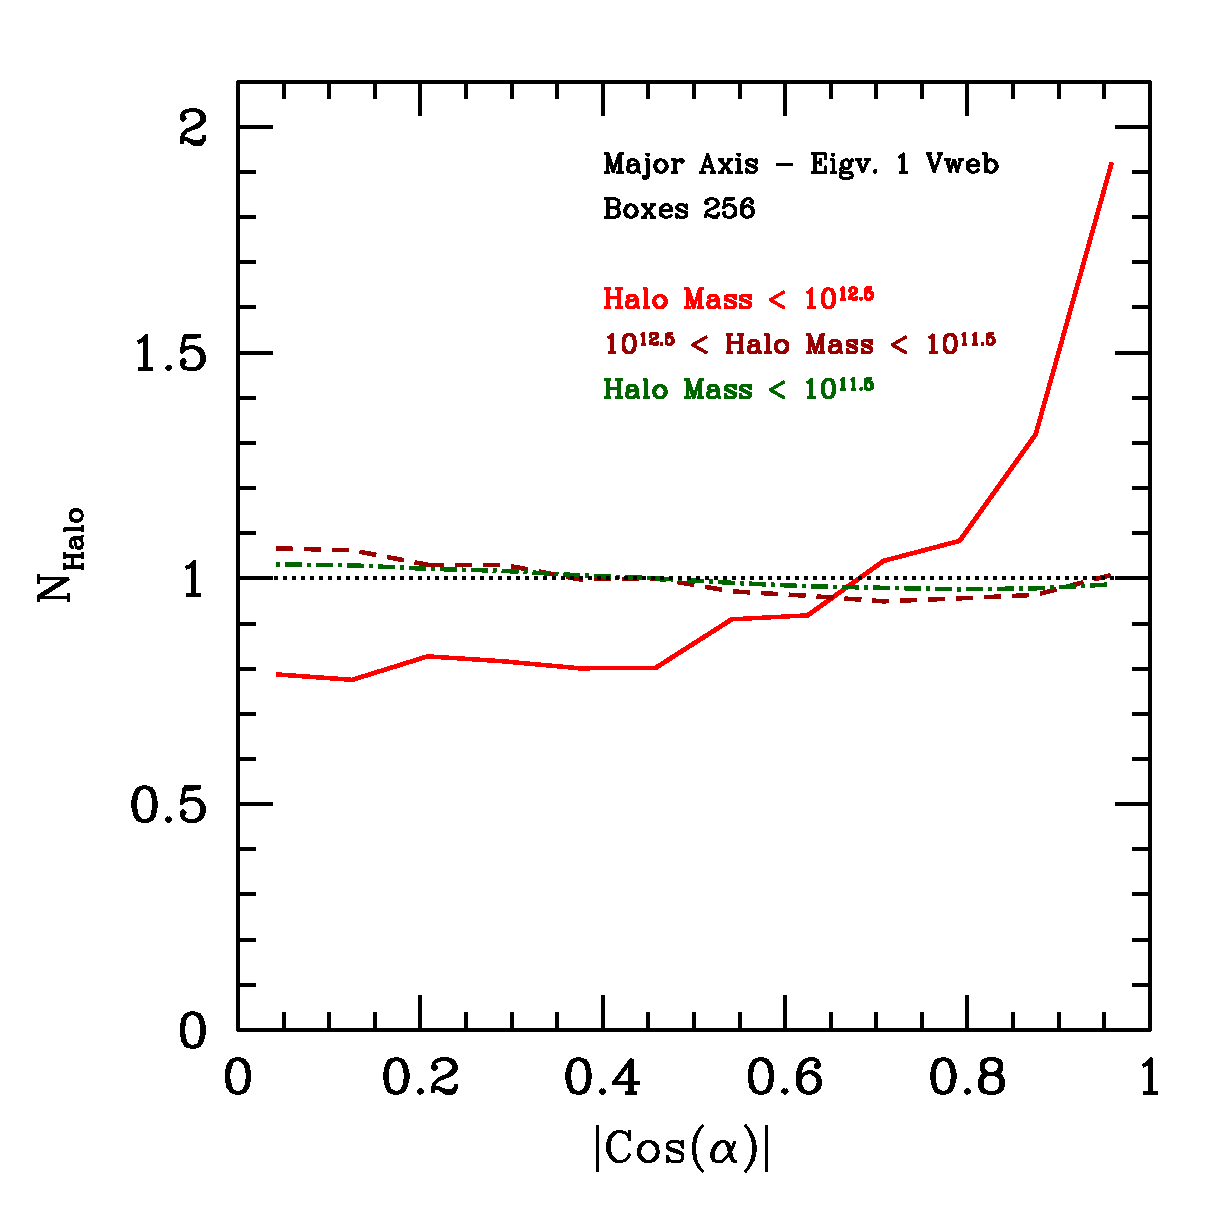
\includegraphics[width=0.30\textwidth]{../plot2/Ax1_VT/256_AX1_V1.ps}
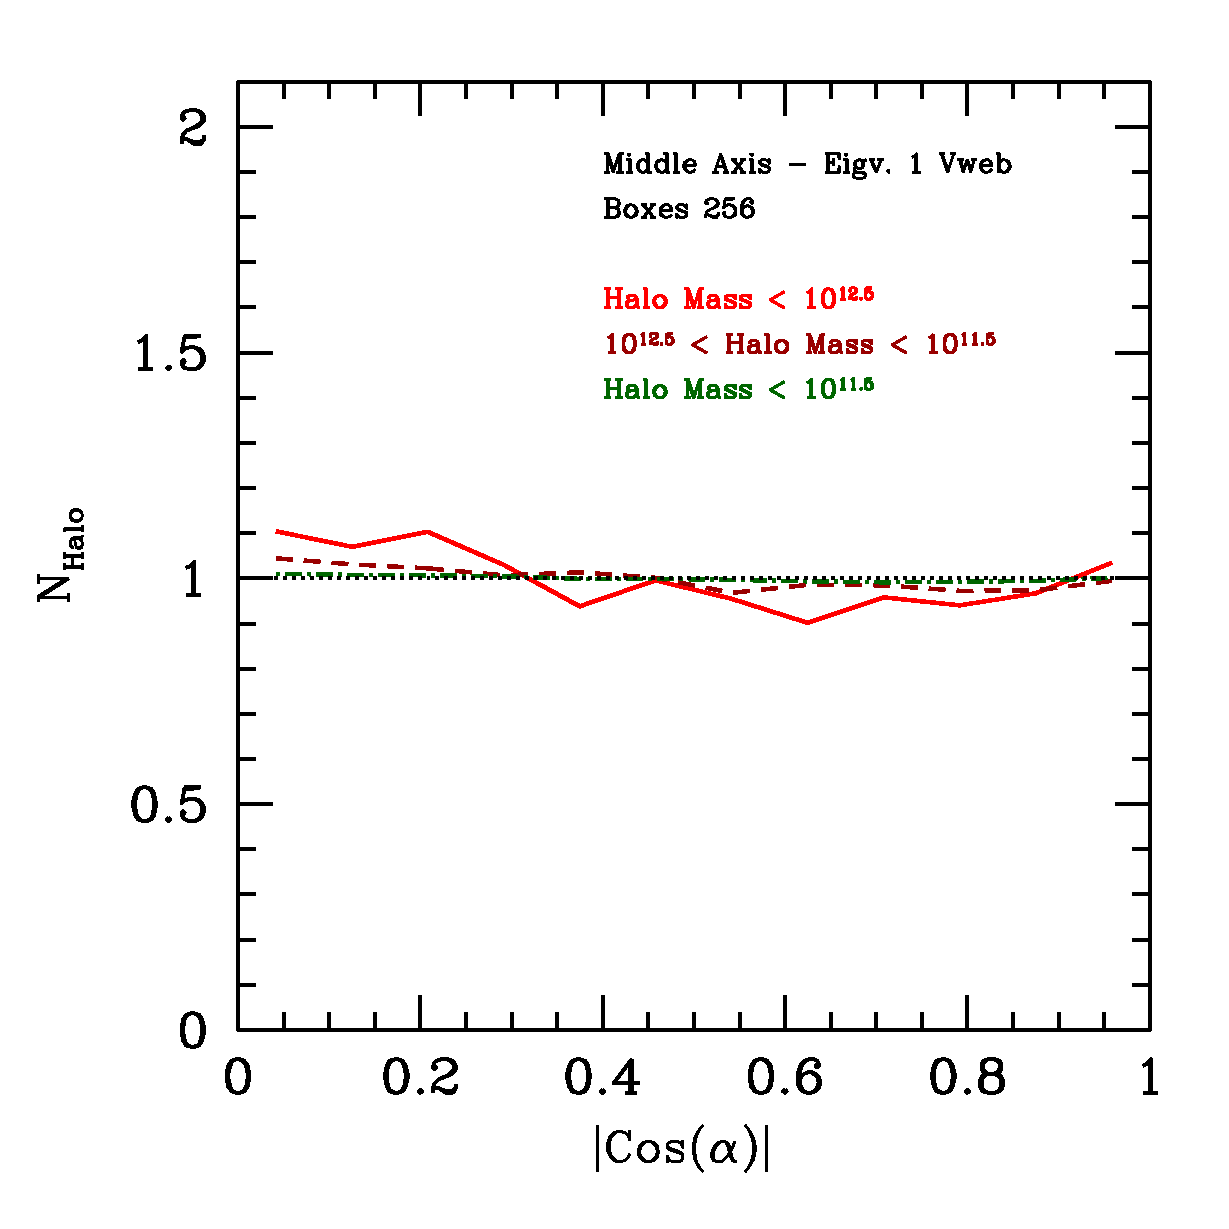
\includegraphics[width=0.30\textwidth]{../plot2/Ax2_VT/256_AX2_V1.ps}
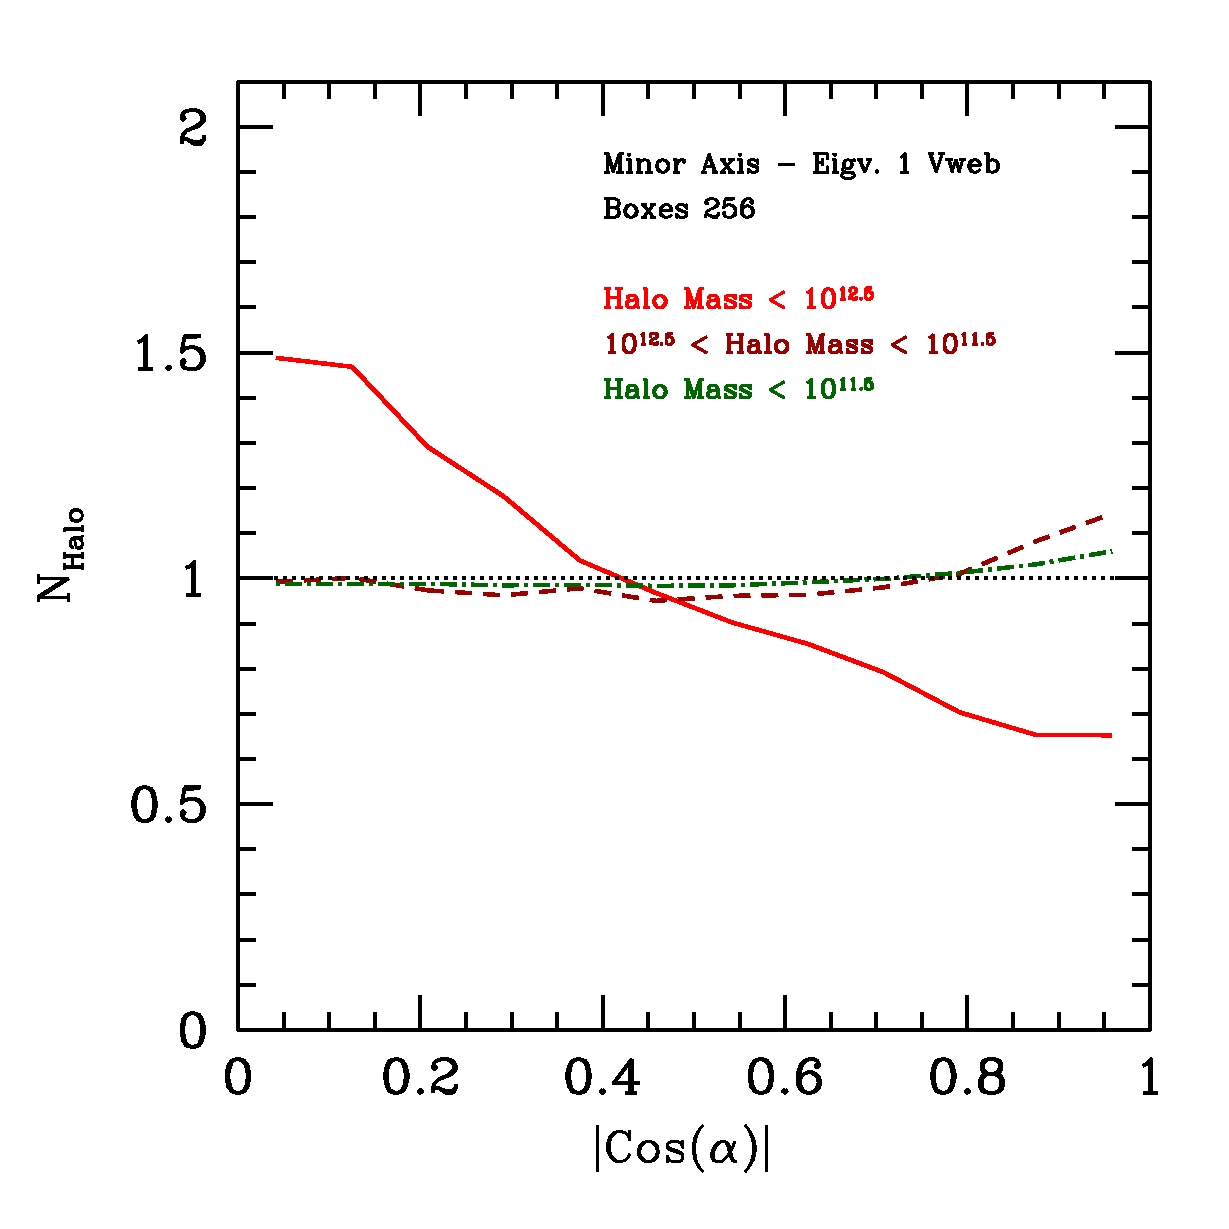
\includegraphics[width=0.30\textwidth]{../plot2/Ax3_VT/256_AX3_V1.ps}
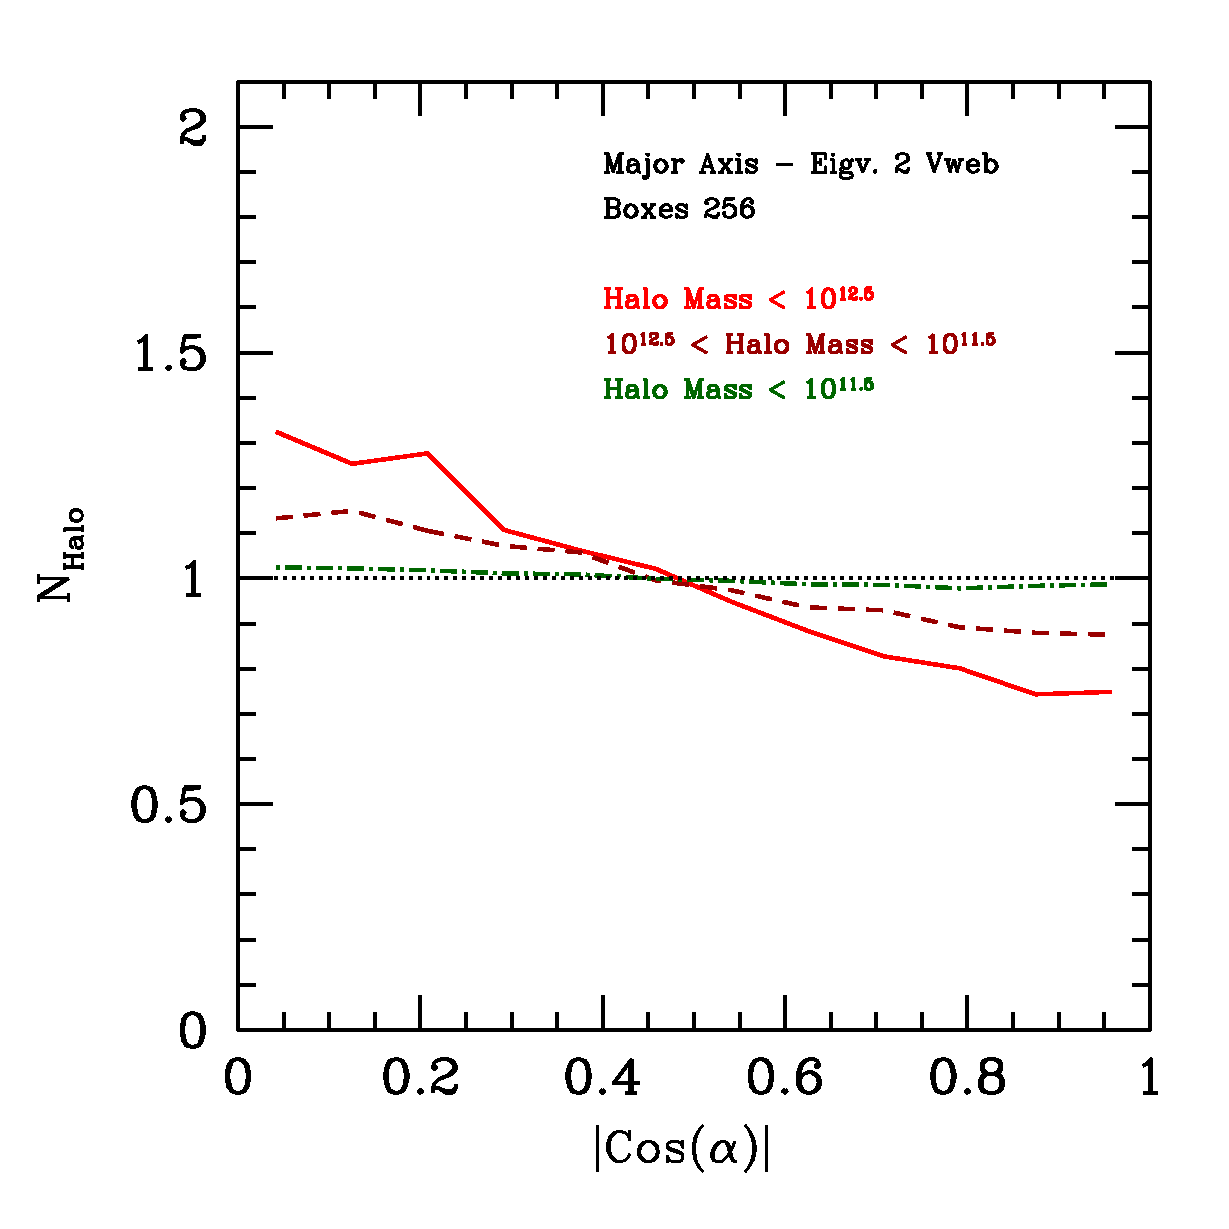
\includegraphics[width=0.30\textwidth]{../plot2/Ax1_VT/256_AX1_V2.ps}
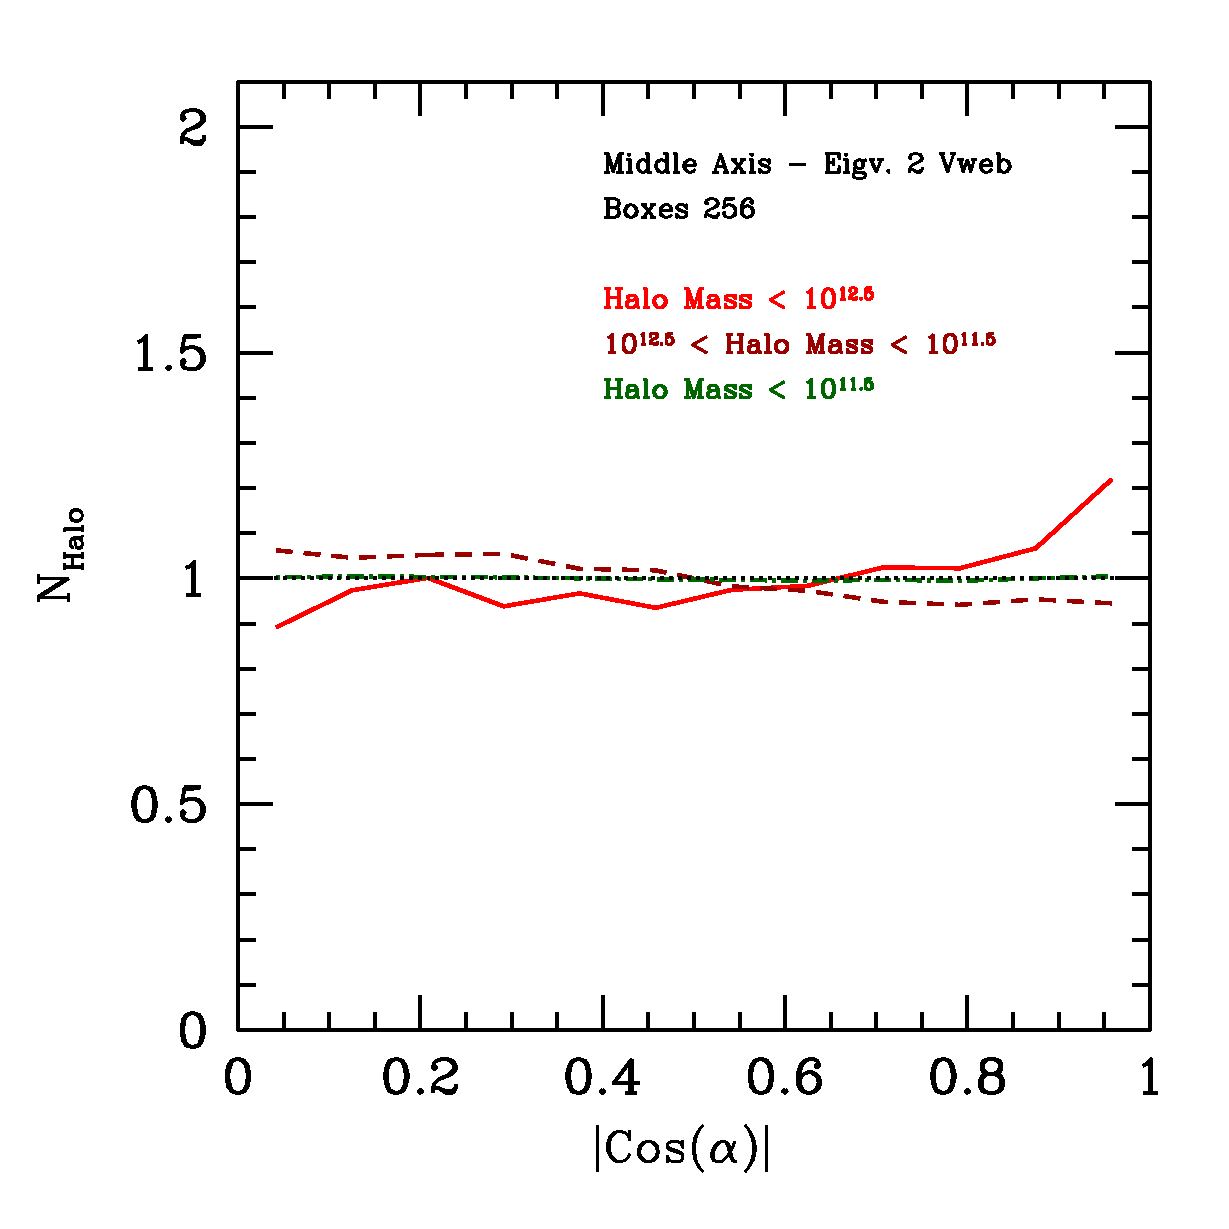
\includegraphics[width=0.30\textwidth]{../plot2/Ax2_VT/256_AX2_V2.ps}
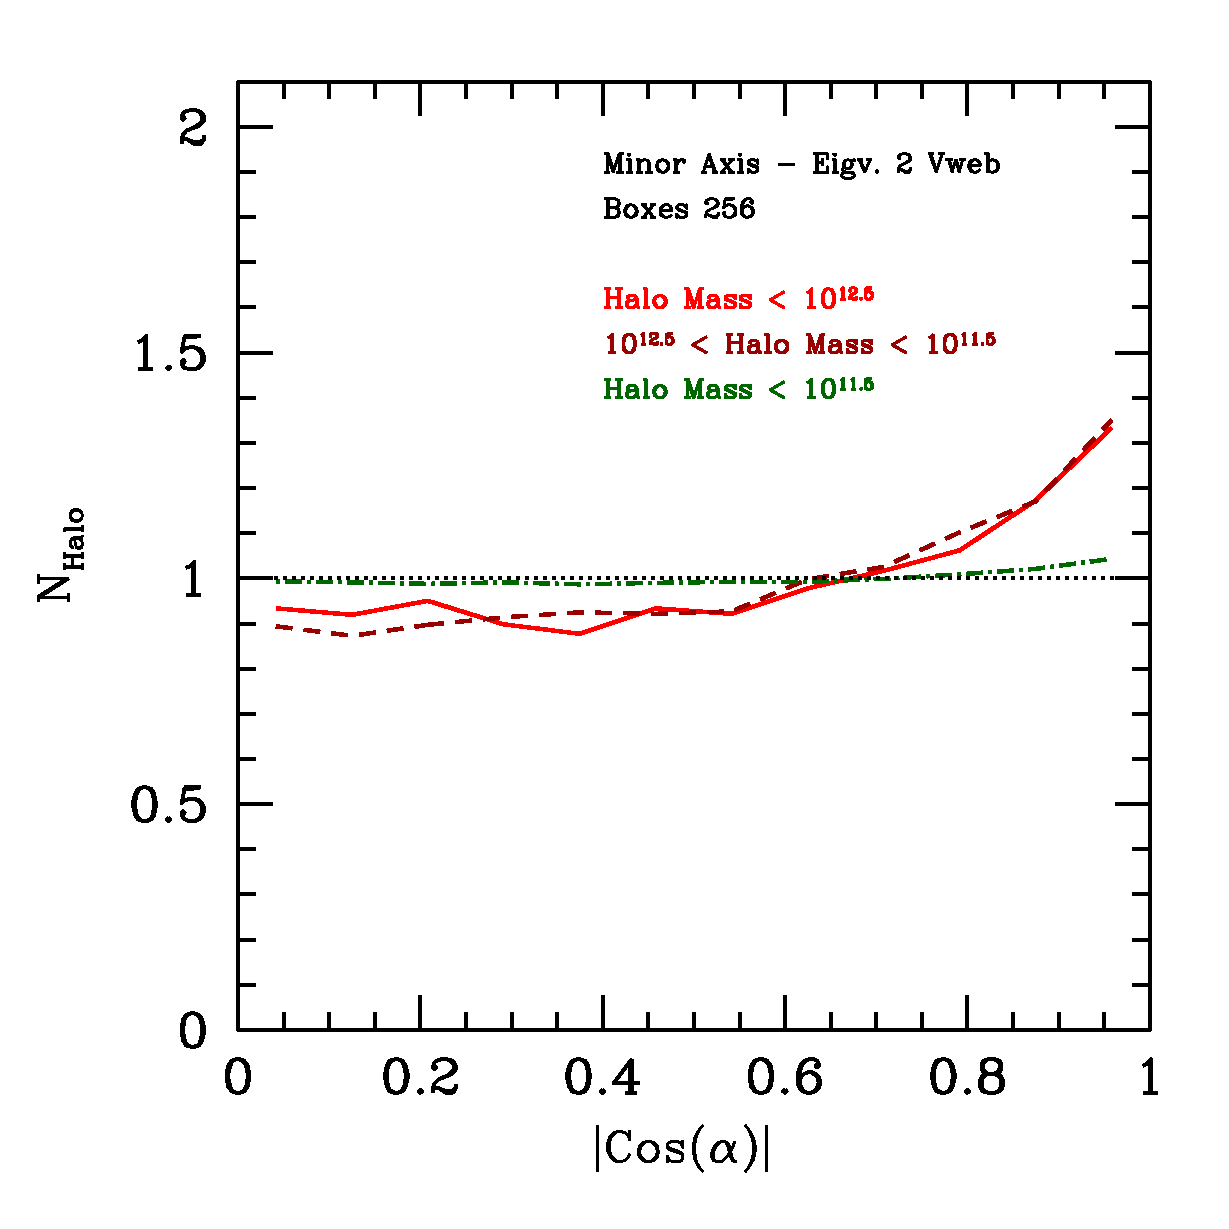
\includegraphics[width=0.30\textwidth]{../plot2/Ax3_VT/256_AX3_V2.ps}
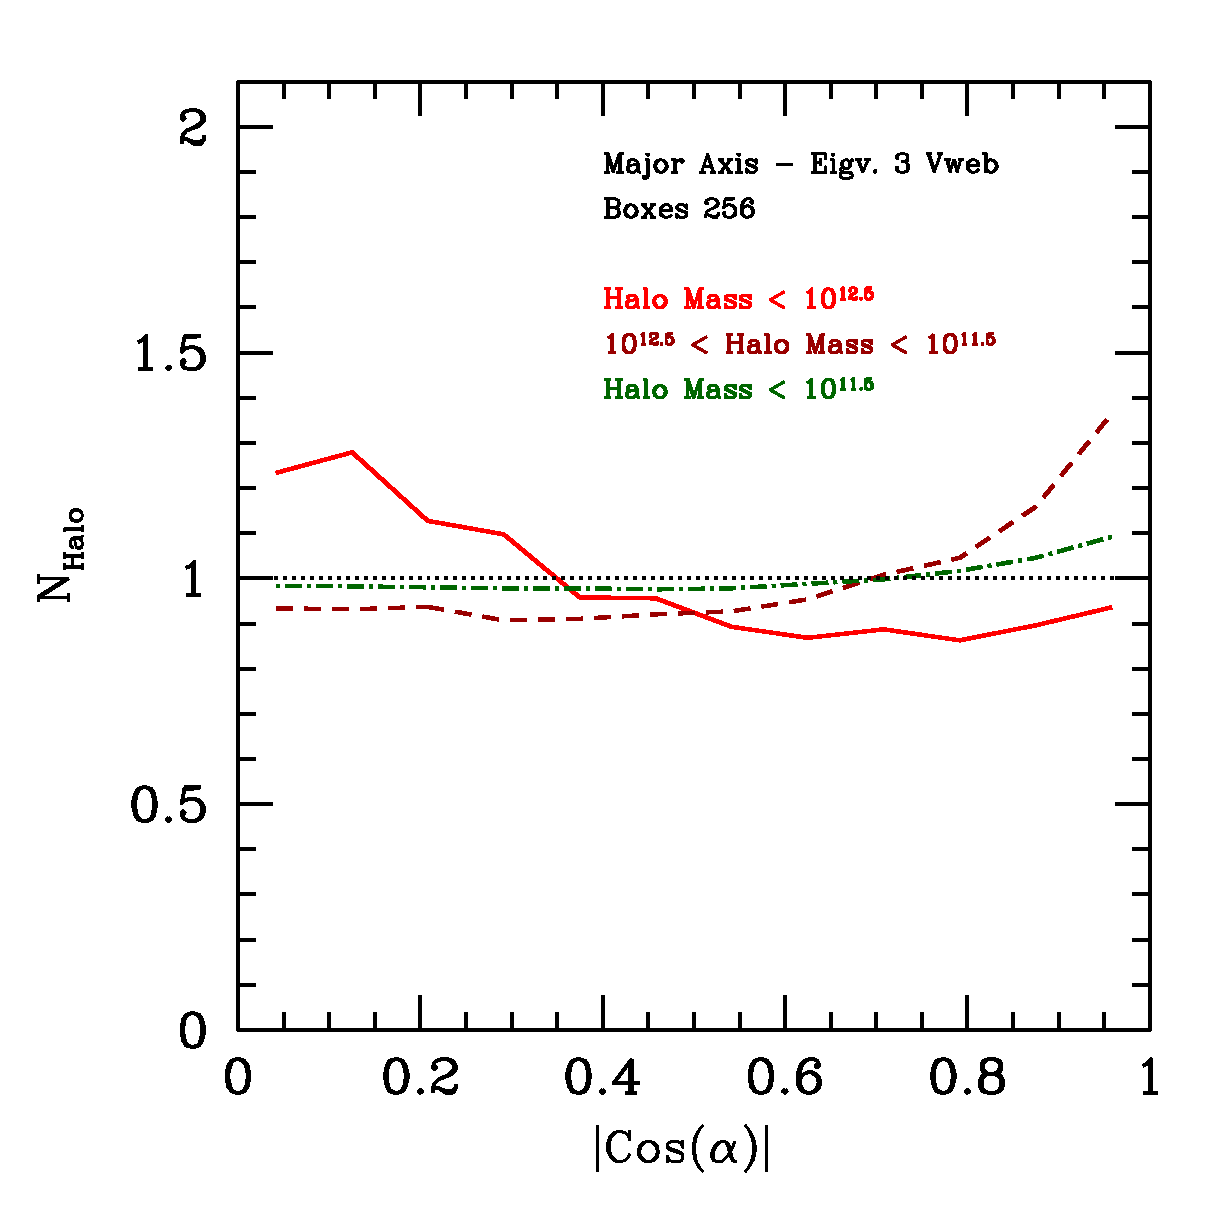
\includegraphics[width=0.30\textwidth]{../plot2/Ax1_VT/256_AX1_V3.ps}
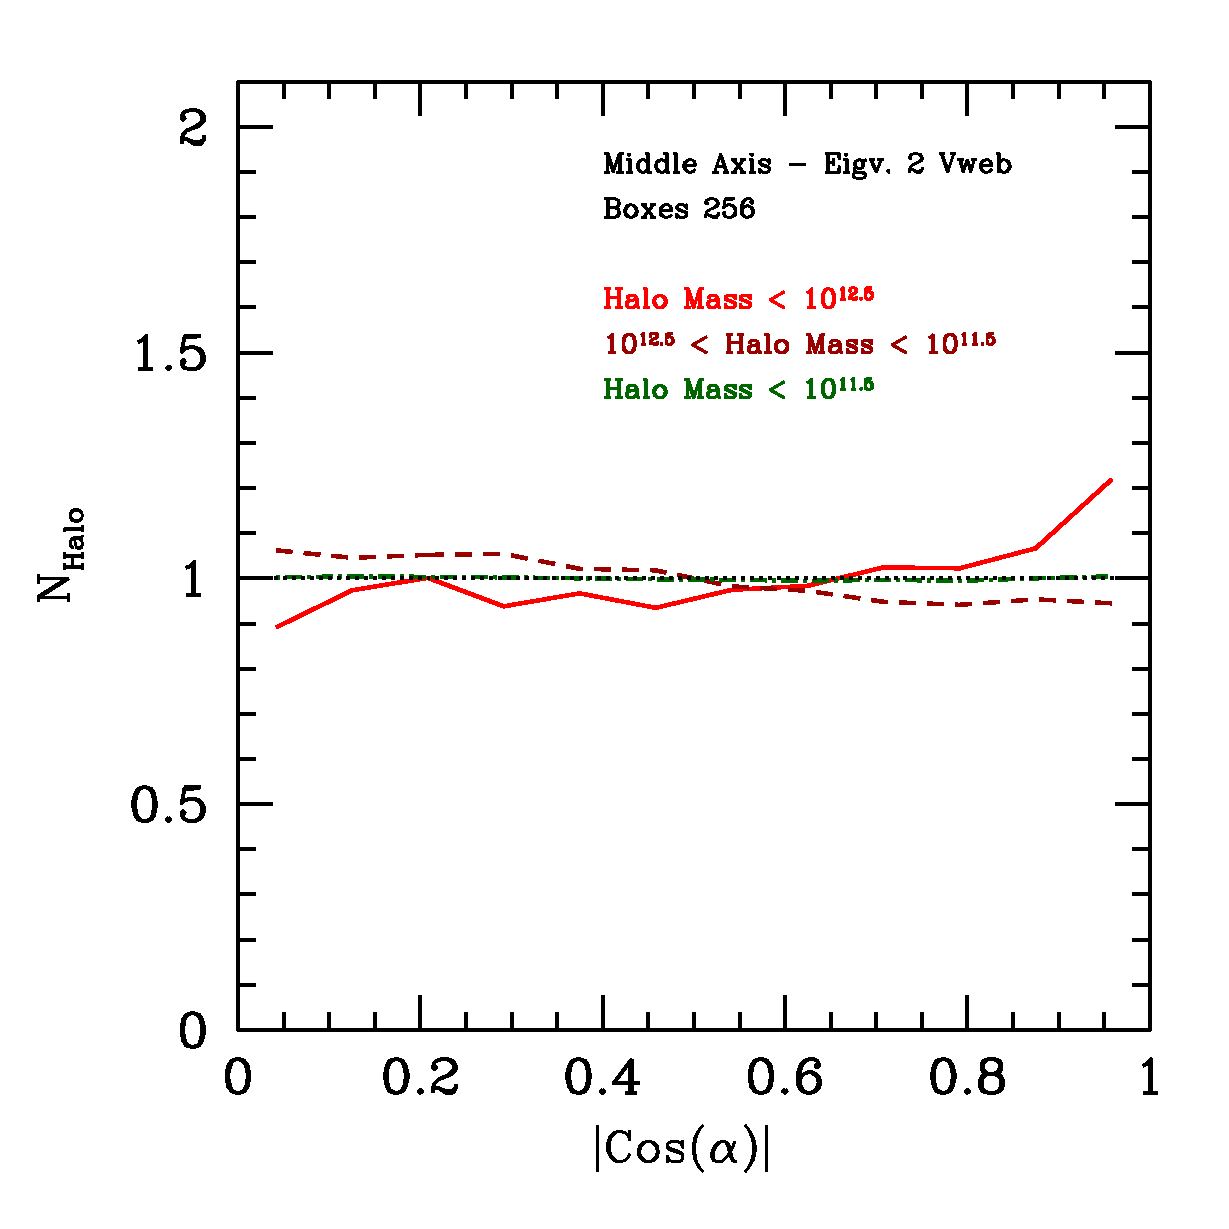
\includegraphics[width=0.30\textwidth]{../plot2/Ax2_VT/256_AX2_V2.ps}
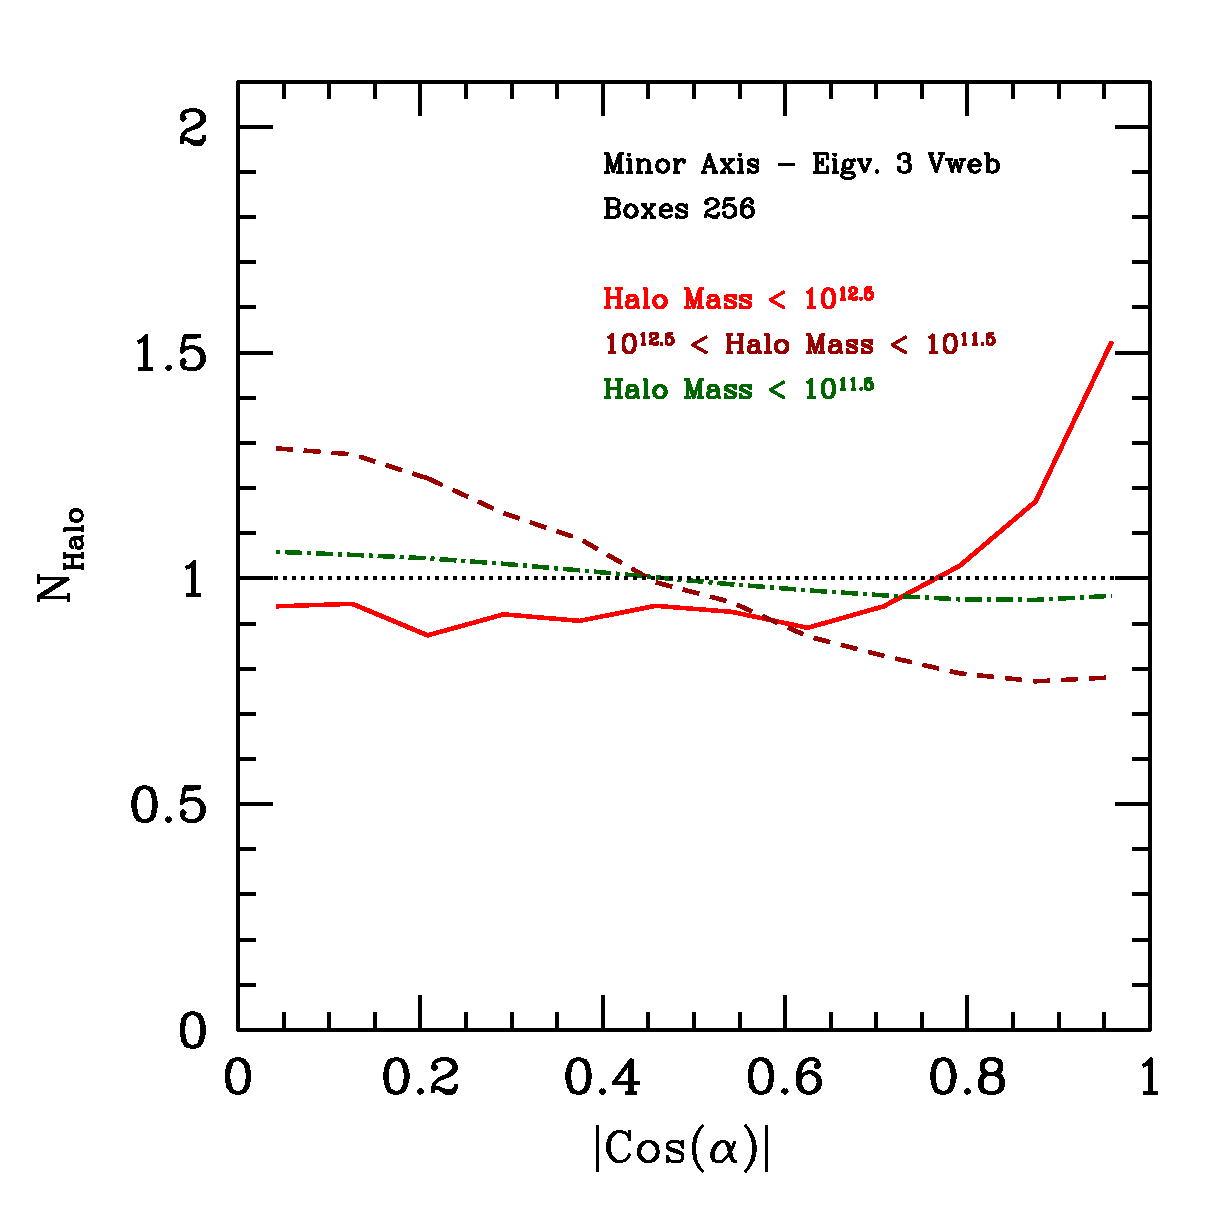
\includegraphics[width=0.30\textwidth]{../plot2/Ax3_VT/256_AX3_V3.ps}
\caption{Shape alignment for the vweb at $256^3$ resolution.}
\end{figure*}

\begin{figure*}
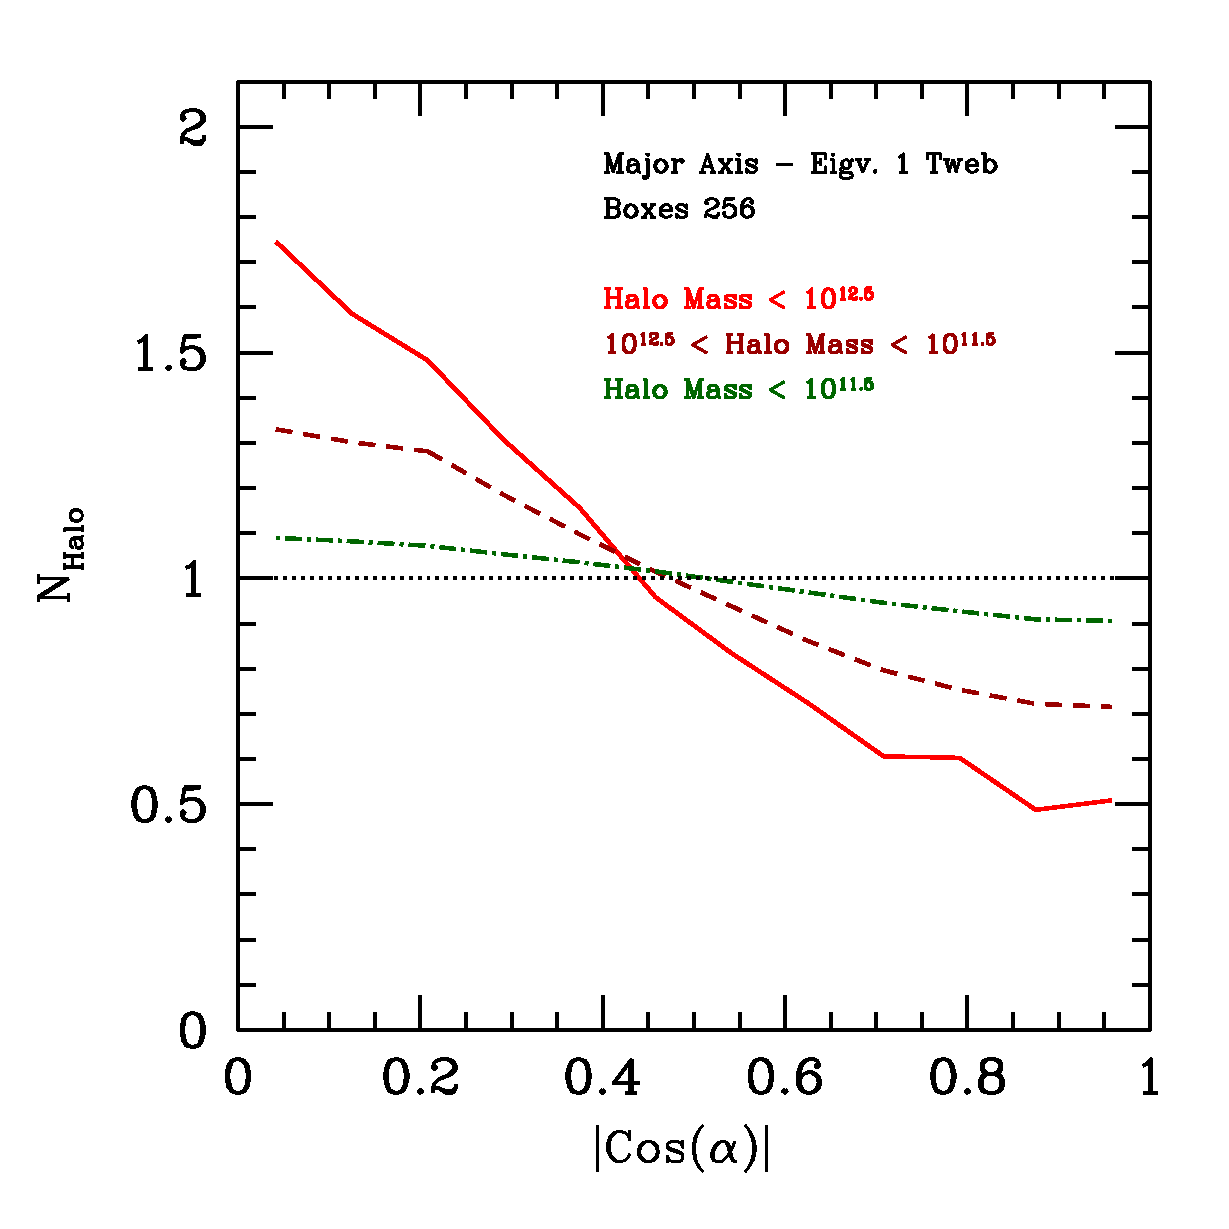
\includegraphics[width=0.30\textwidth]{../plot2/Ax1_VT/256_AX1_T1.ps}
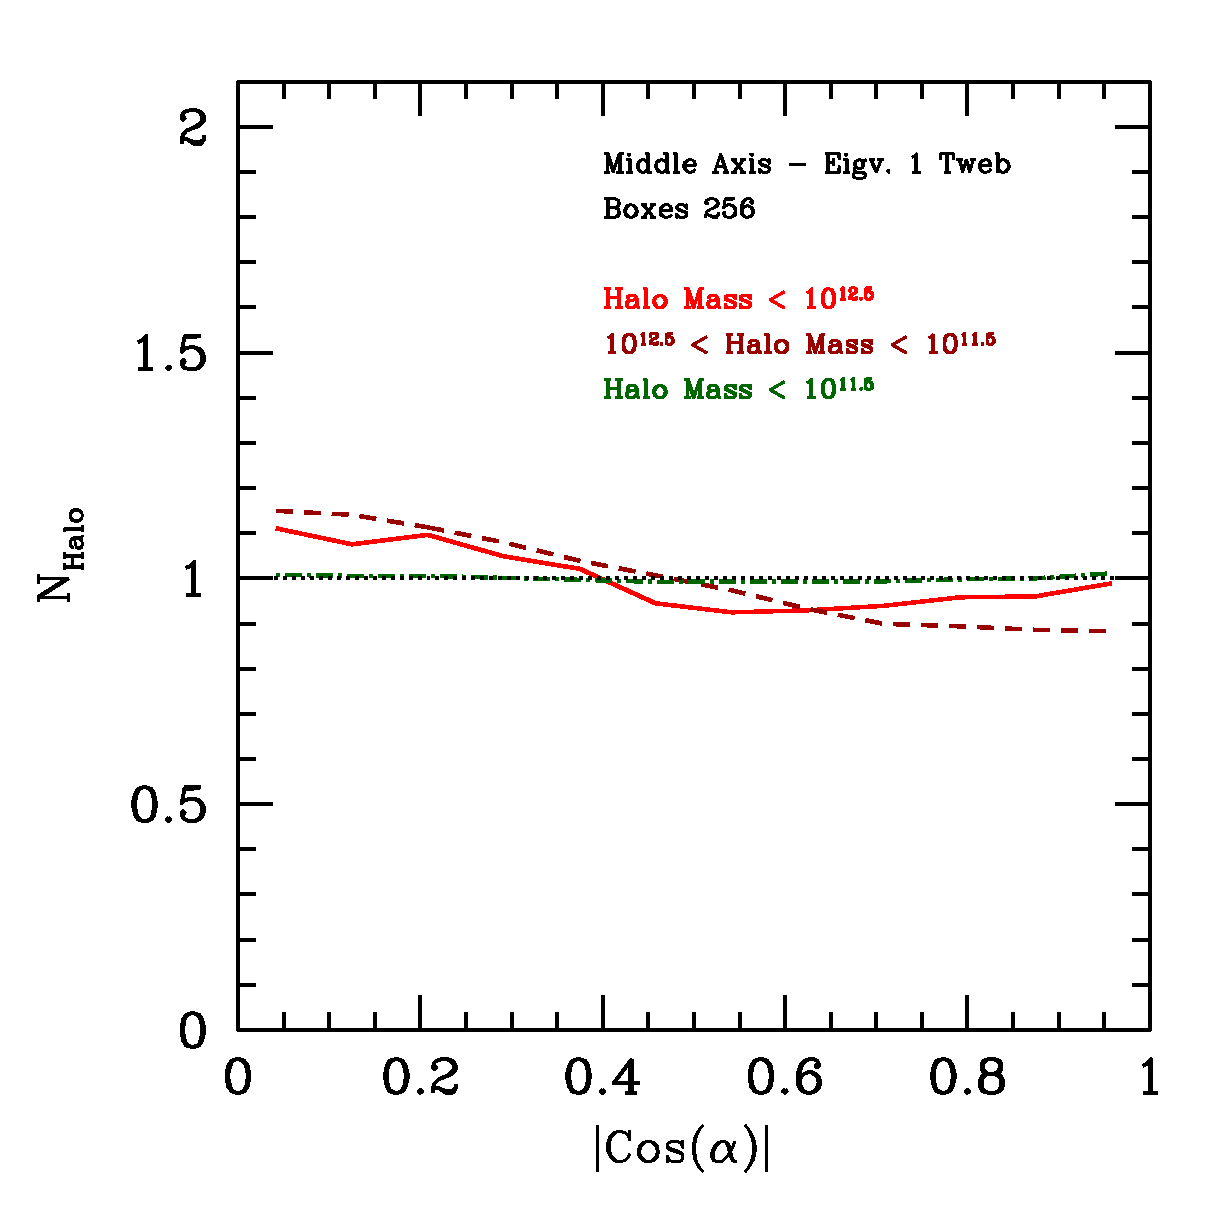
\includegraphics[width=0.30\textwidth]{../plot2/Ax2_VT/256_AX2_T1.ps}
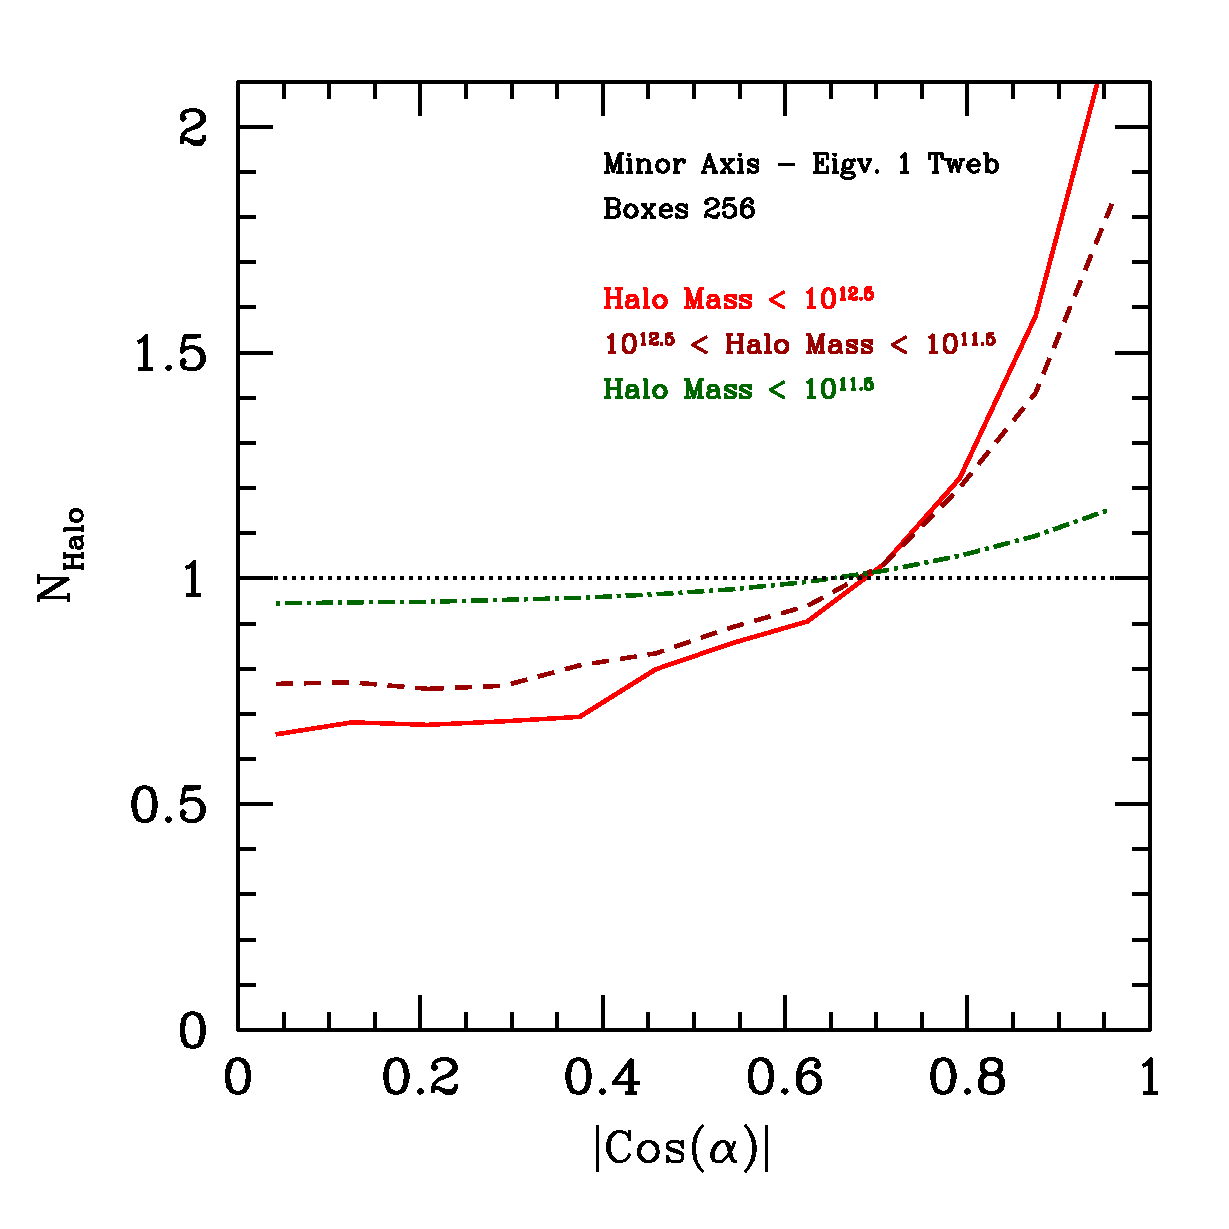
\includegraphics[width=0.30\textwidth]{../plot2/Ax3_VT/256_AX3_T1.ps}
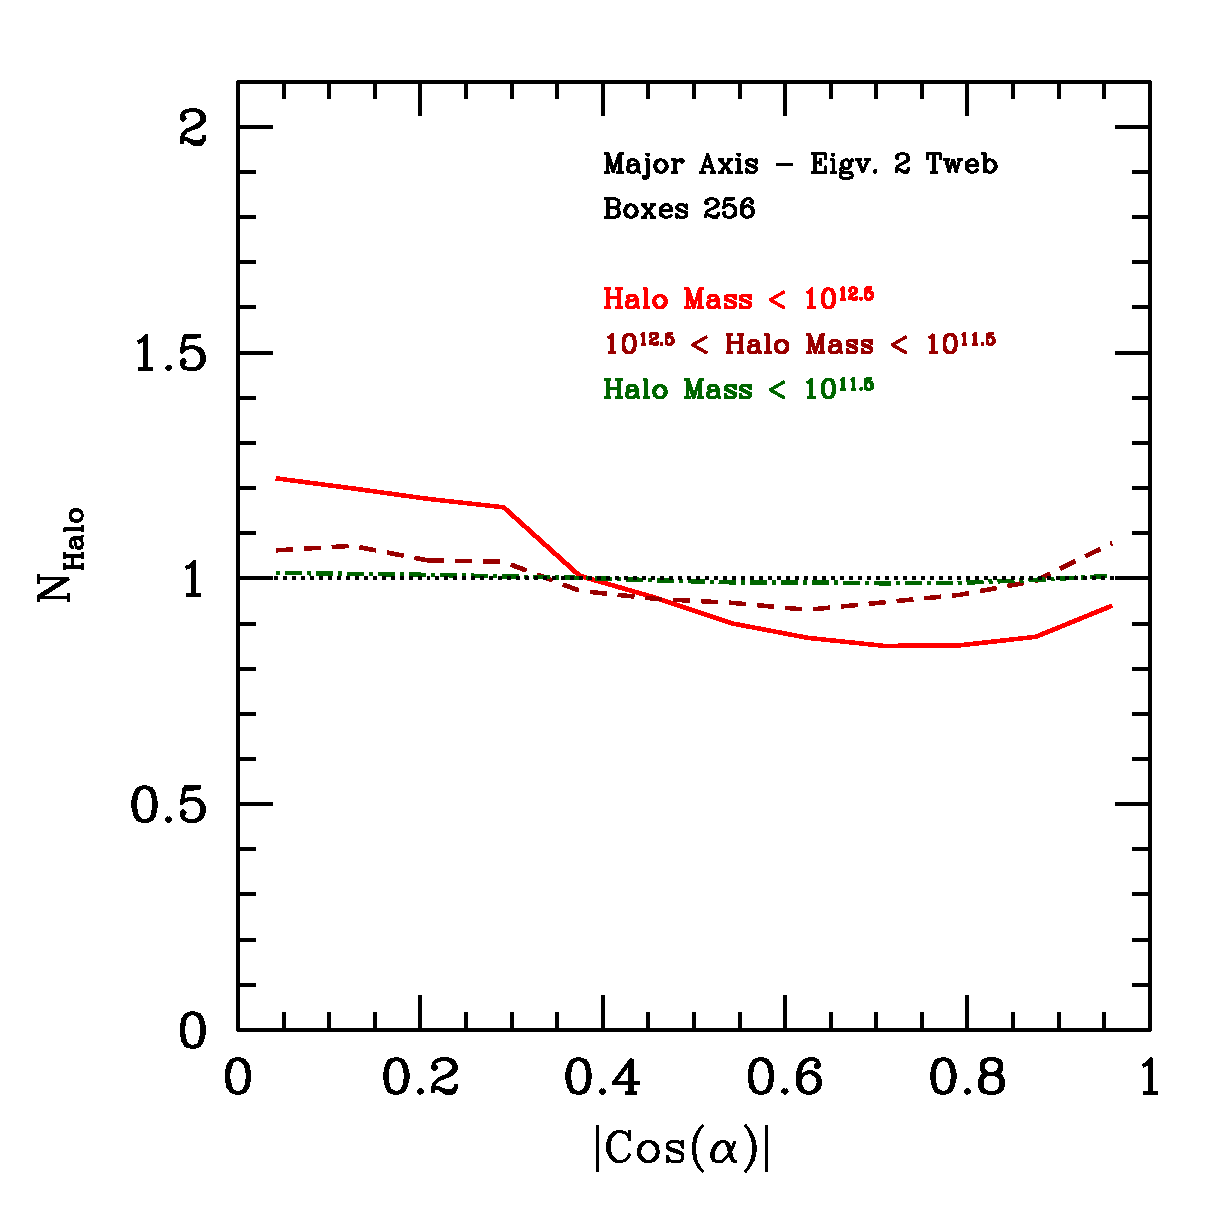
\includegraphics[width=0.30\textwidth]{../plot2/Ax1_VT/256_AX1_T2.ps}
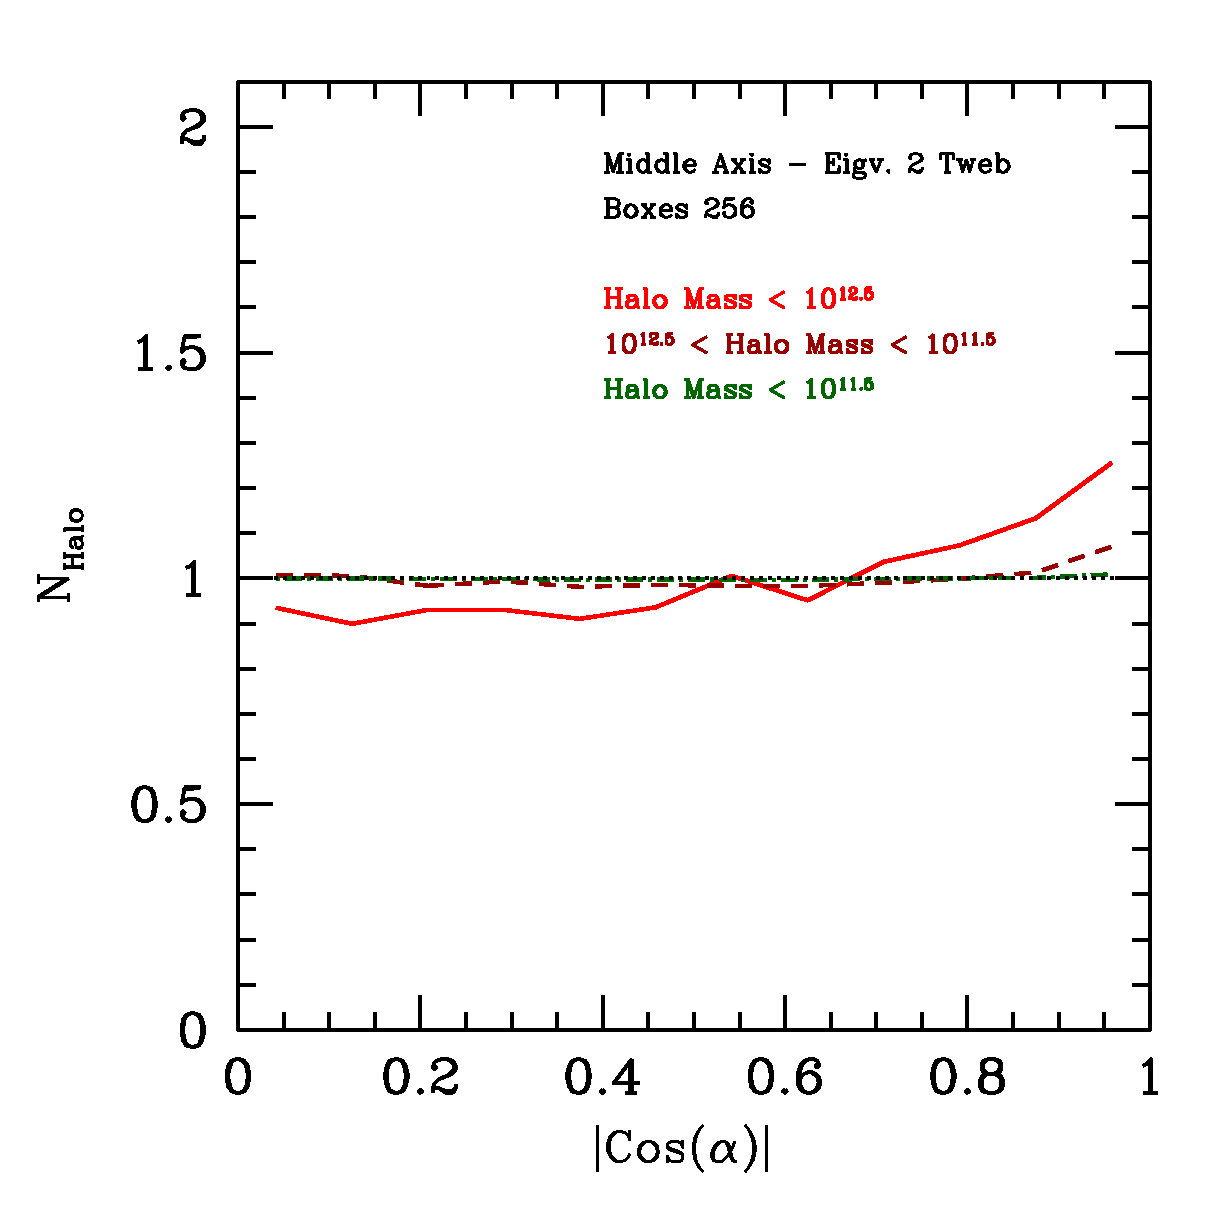
\includegraphics[width=0.30\textwidth]{../plot2/Ax2_VT/256_AX2_T2.ps}
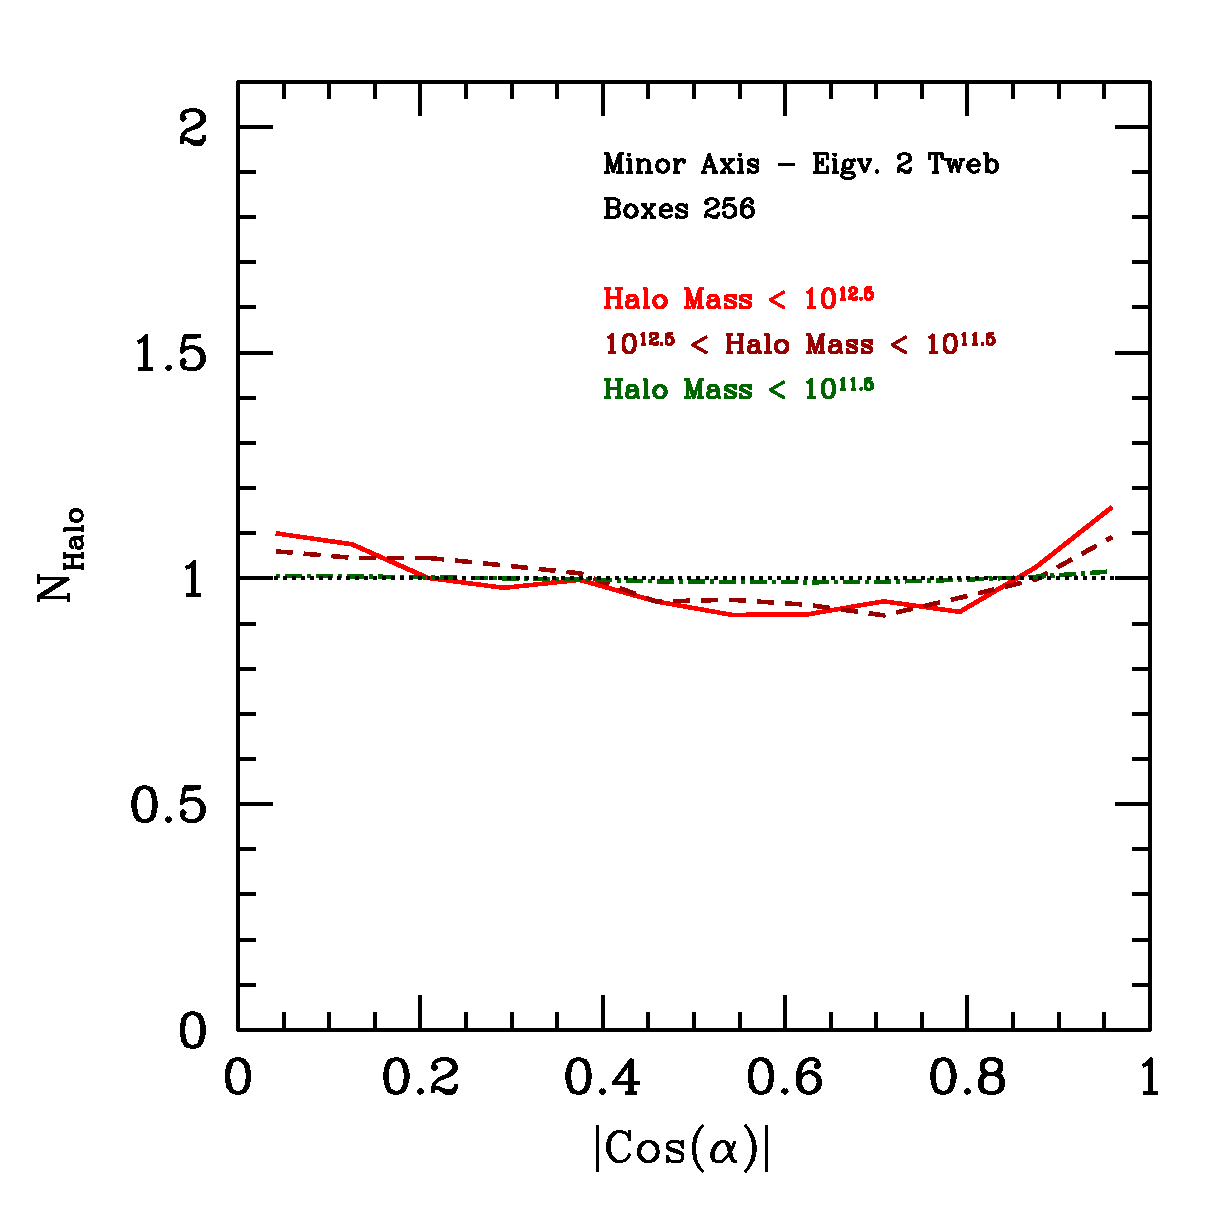
\includegraphics[width=0.30\textwidth]{../plot2/Ax3_VT/256_AX3_T2.ps}
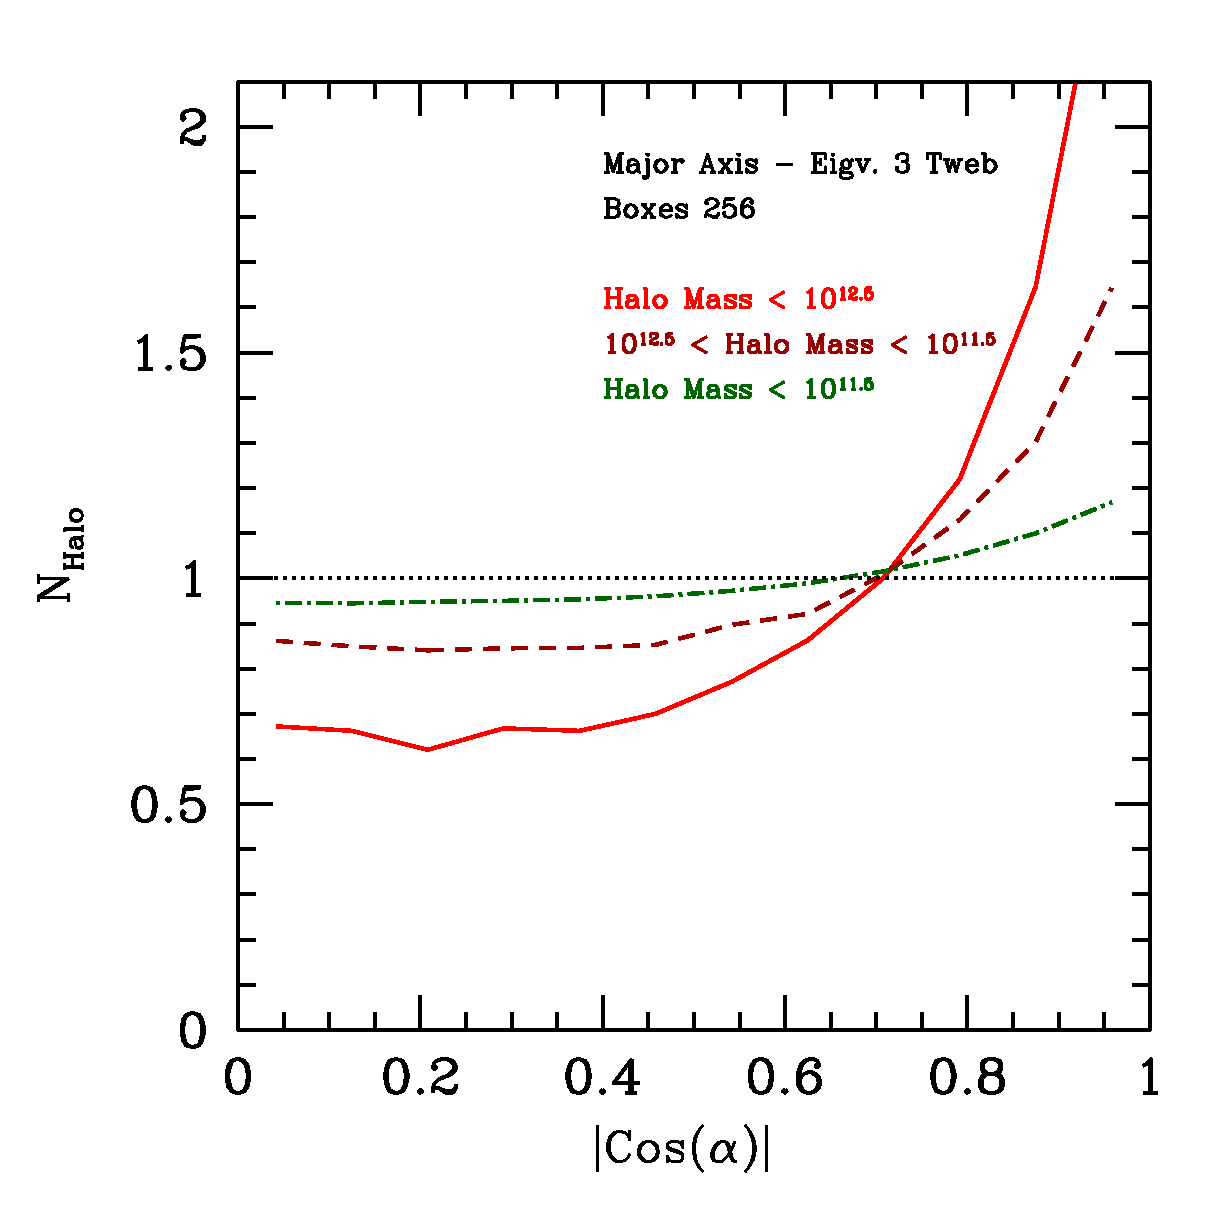
\includegraphics[width=0.30\textwidth]{../plot2/Ax1_VT/256_AX1_T3.ps}
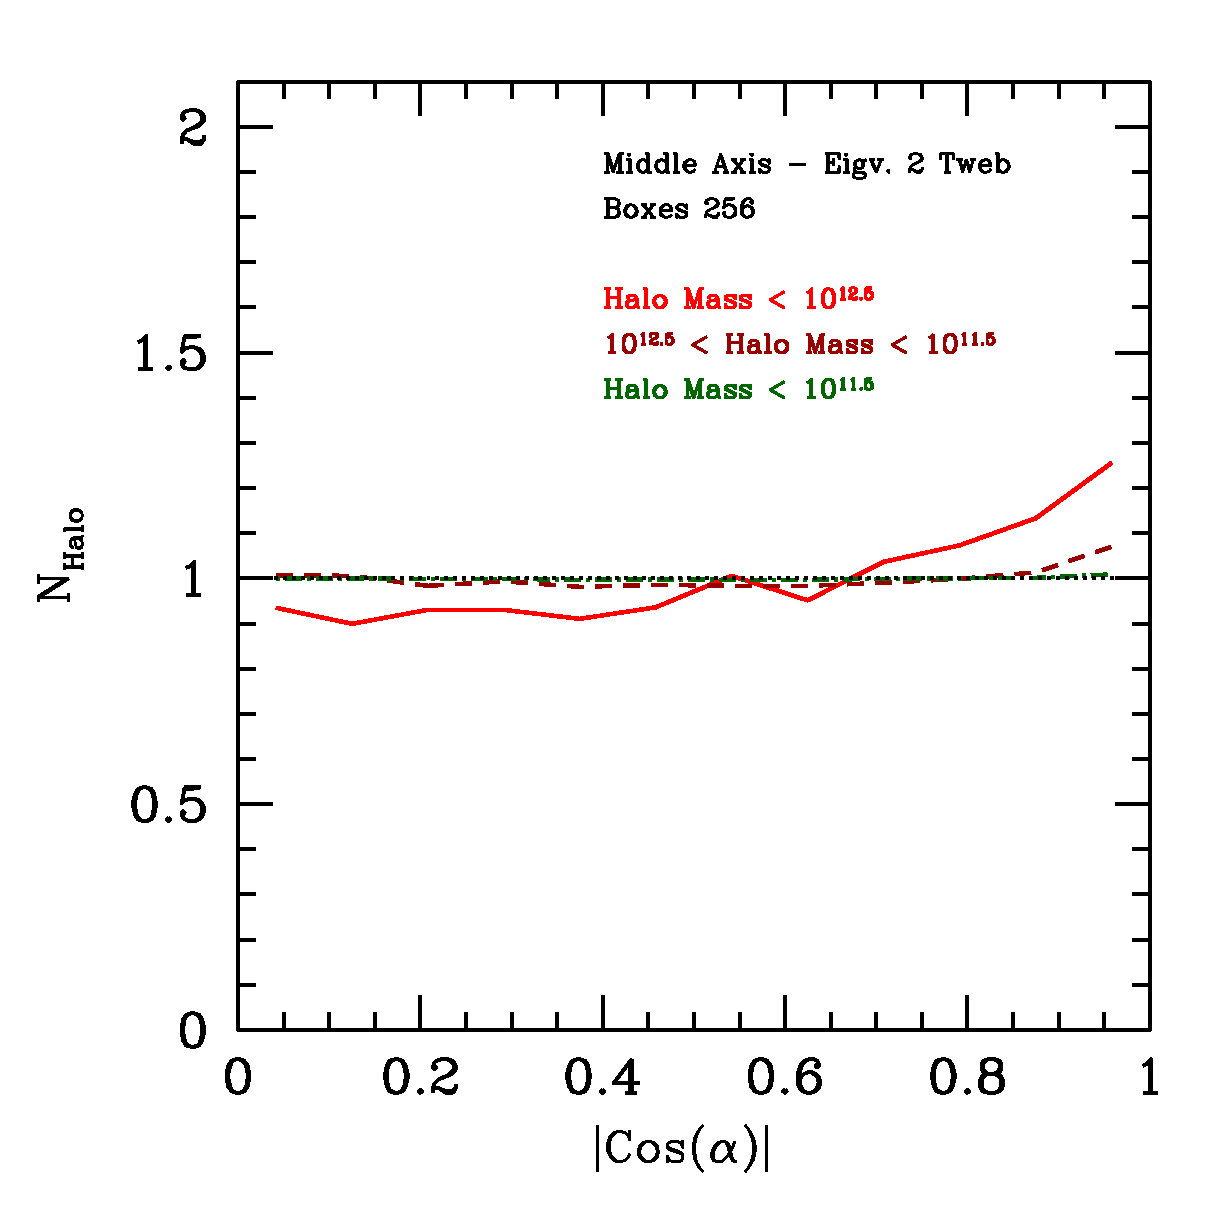
\includegraphics[width=0.30\textwidth]{../plot2/Ax2_VT/256_AX2_T2.ps}
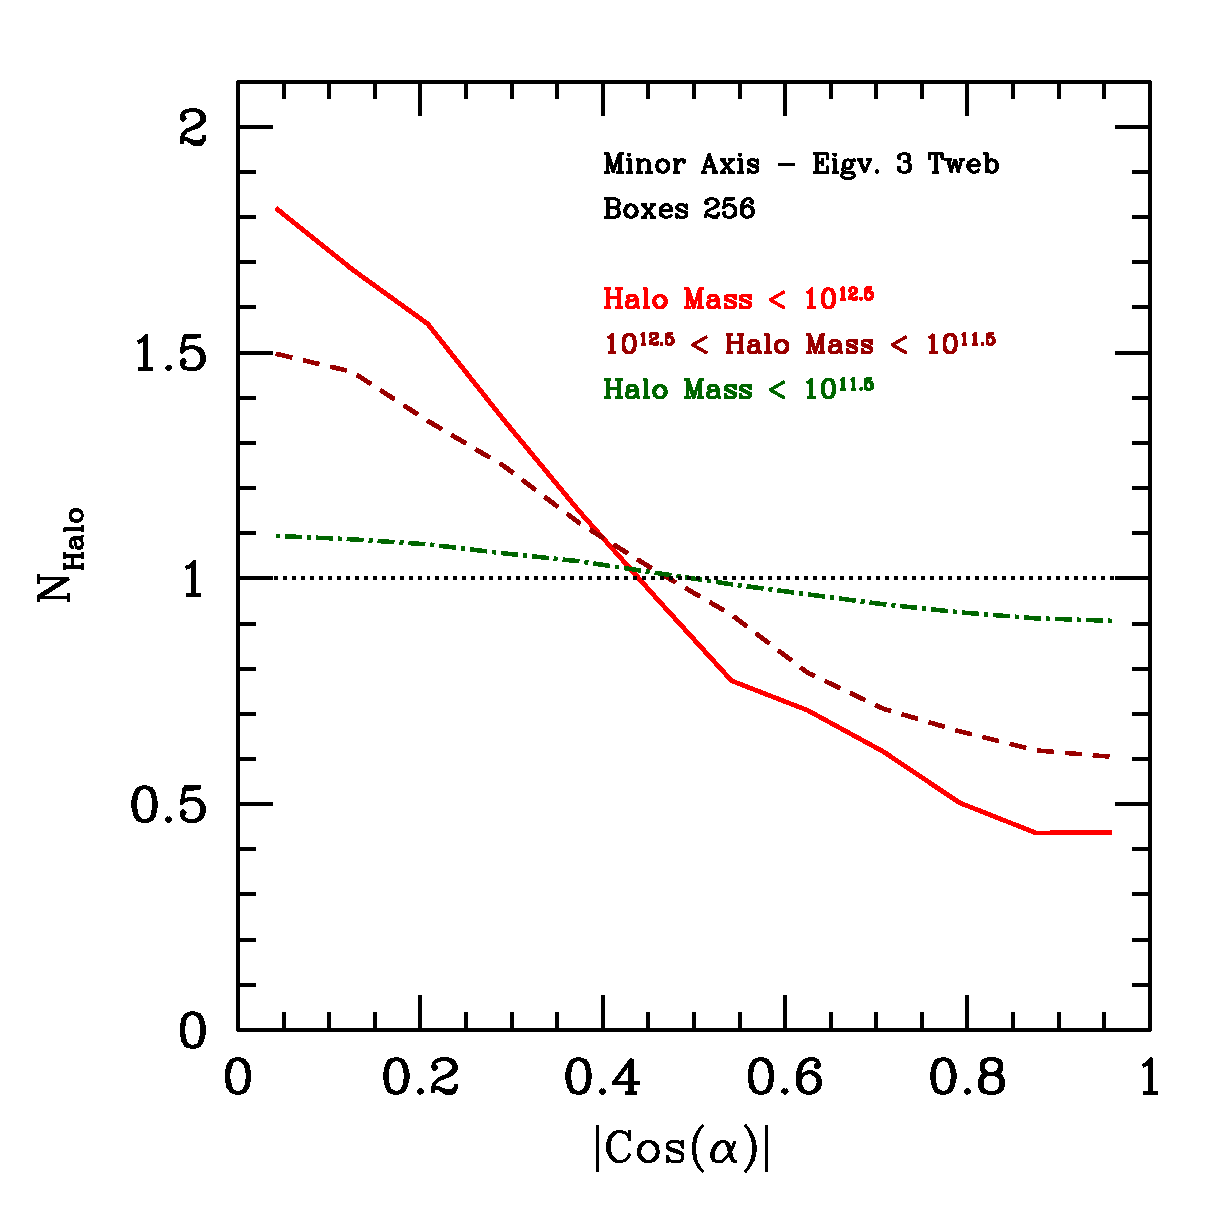
\includegraphics[width=0.30\textwidth]{../plot2/Ax3_VT/256_AX3_T3.ps}
\caption{Shape alignment for the tweb at $256^3$ resolution.}
\end{figure*}


\begin{figure*}
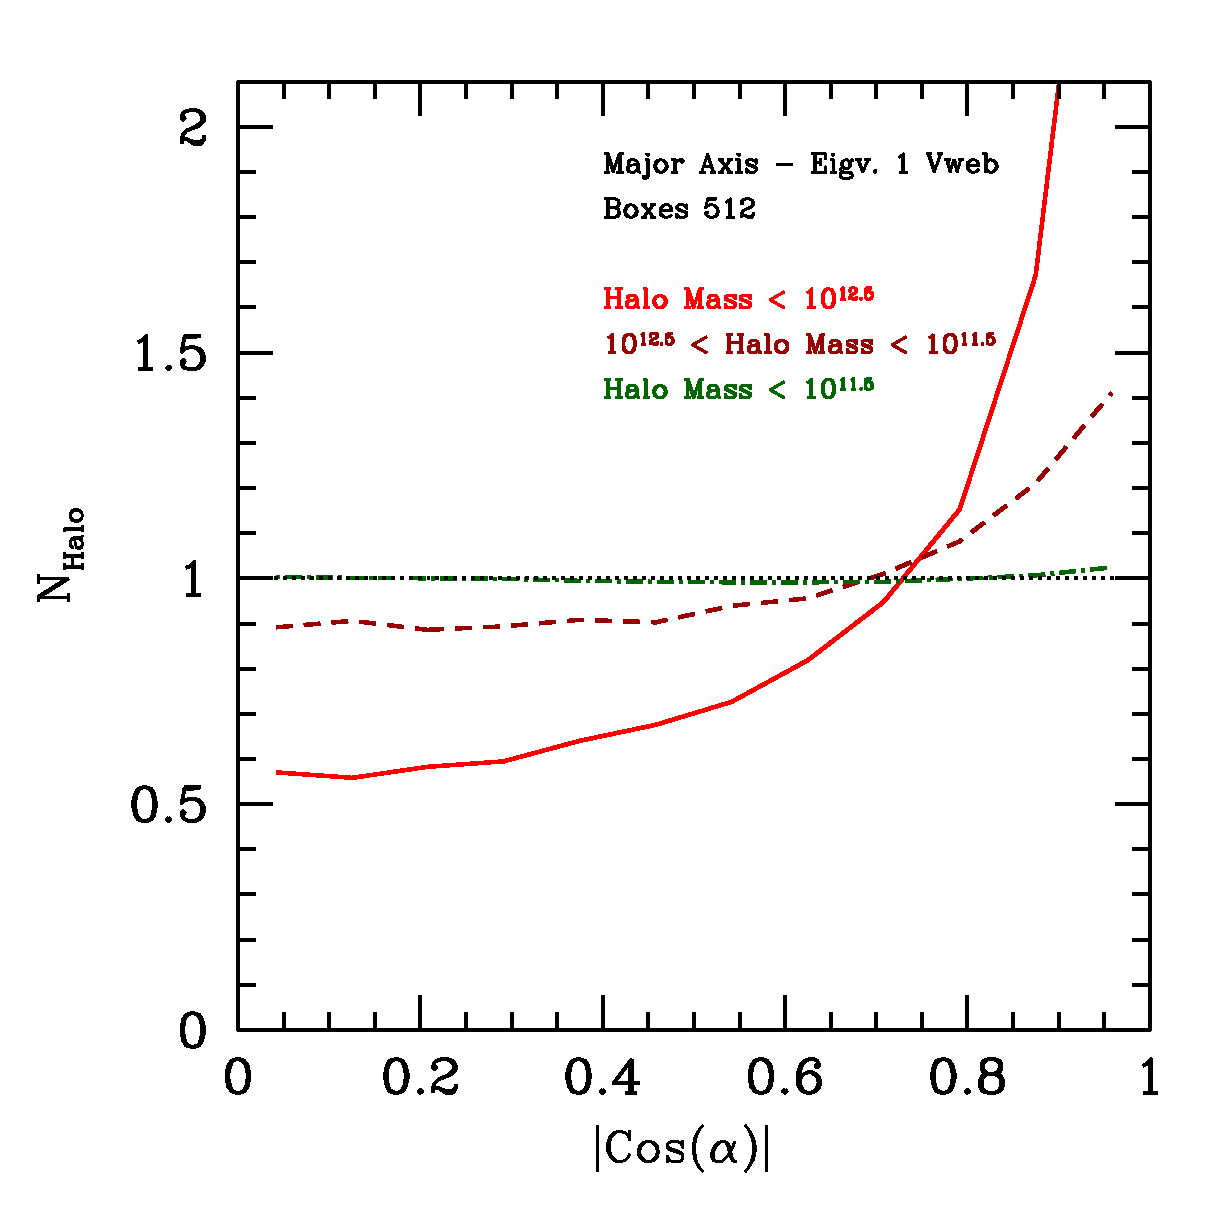
\includegraphics[width=0.30\textwidth]{../plot2/Ax1_VT/512_AX1_V1.ps}
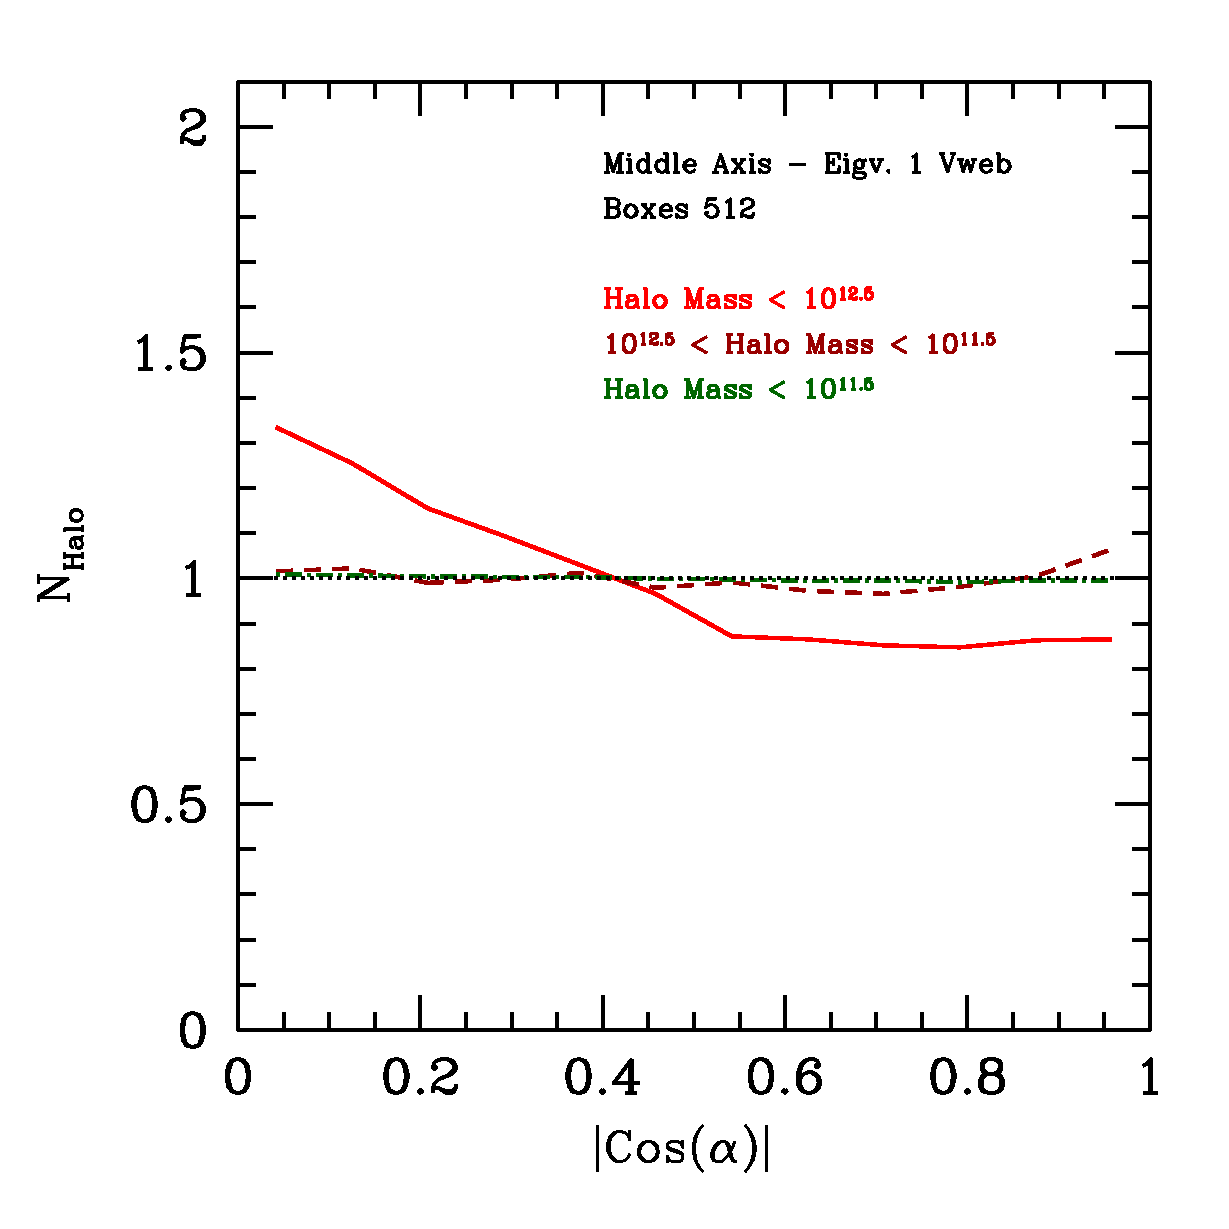
\includegraphics[width=0.30\textwidth]{../plot2/Ax2_VT/512_AX2_V1.ps}
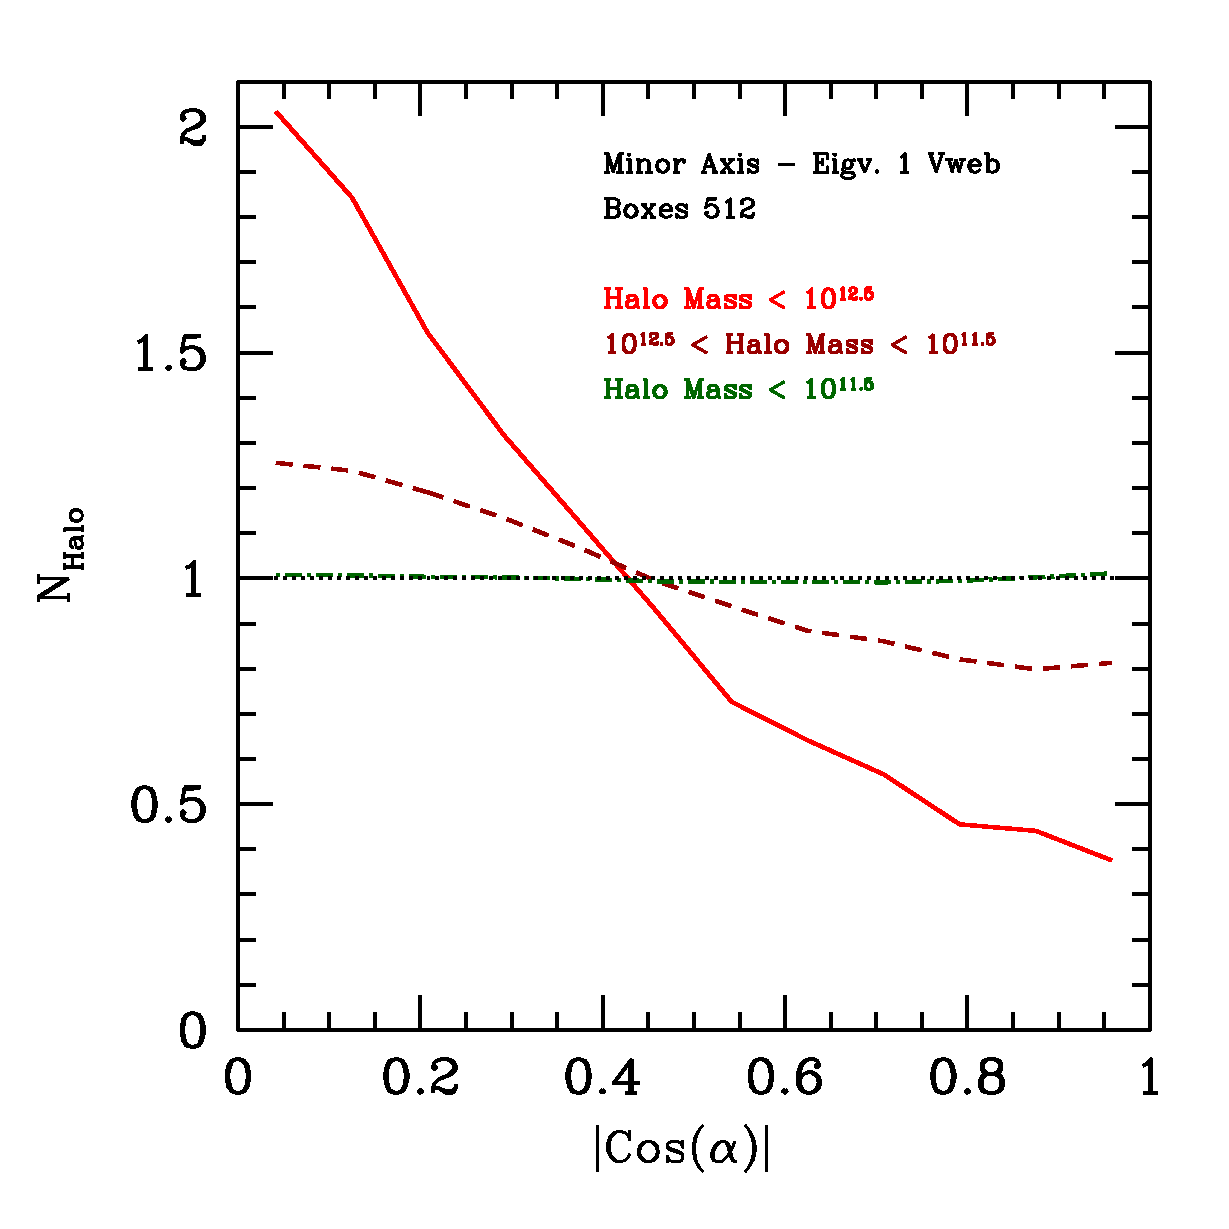
\includegraphics[width=0.30\textwidth]{../plot2/Ax3_VT/512_AX3_V1.ps}
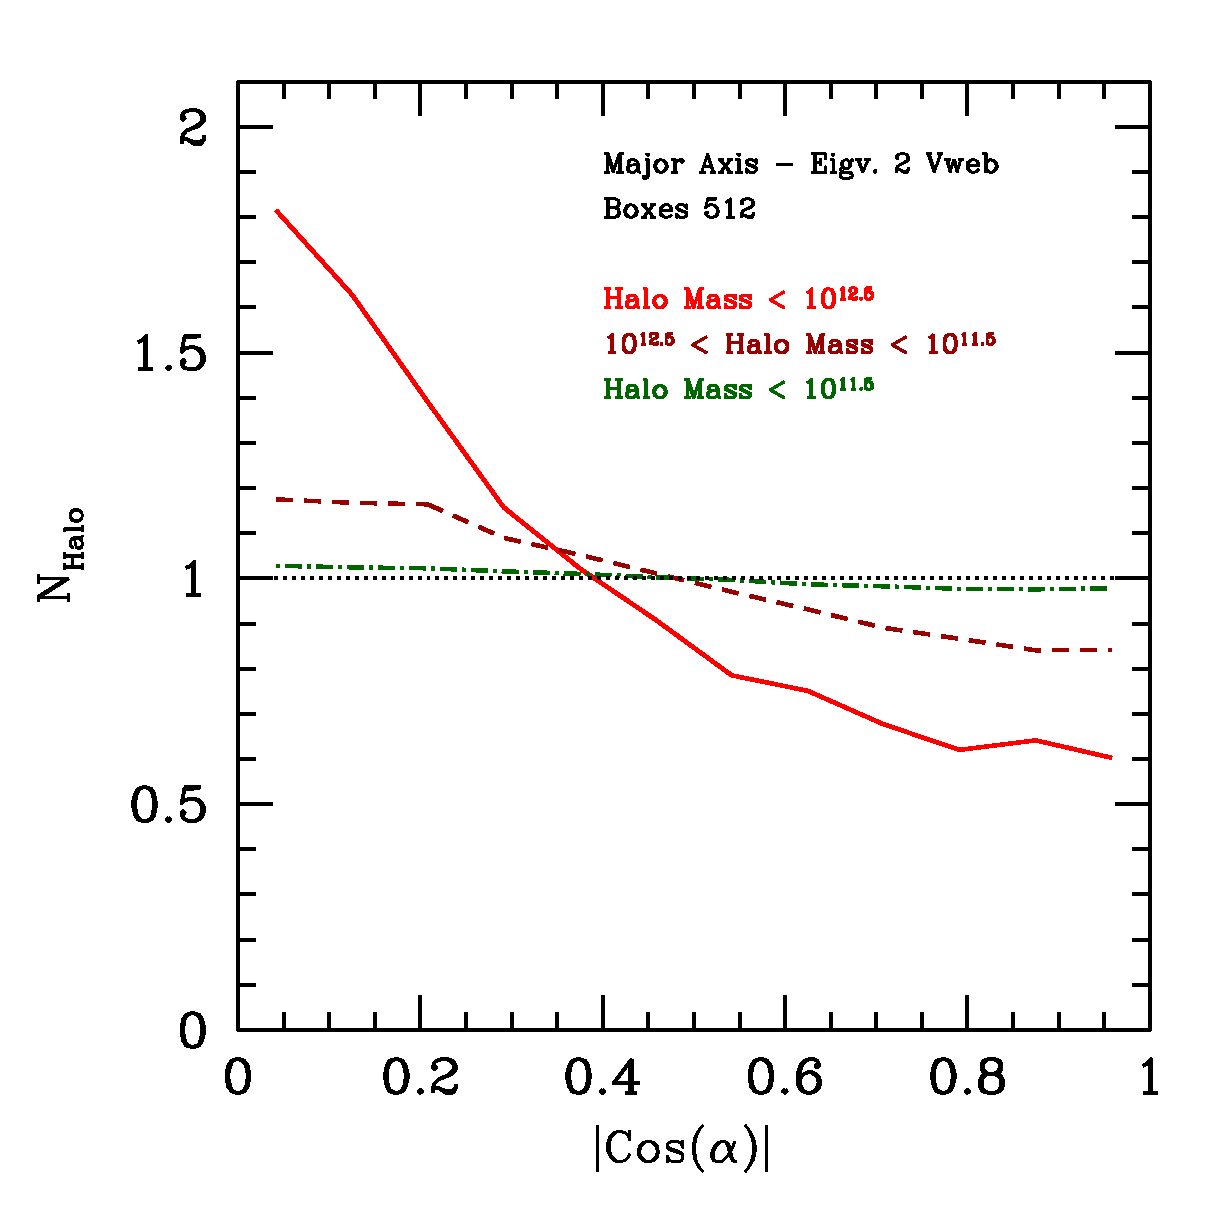
\includegraphics[width=0.30\textwidth]{../plot2/Ax1_VT/512_AX1_V2.ps}
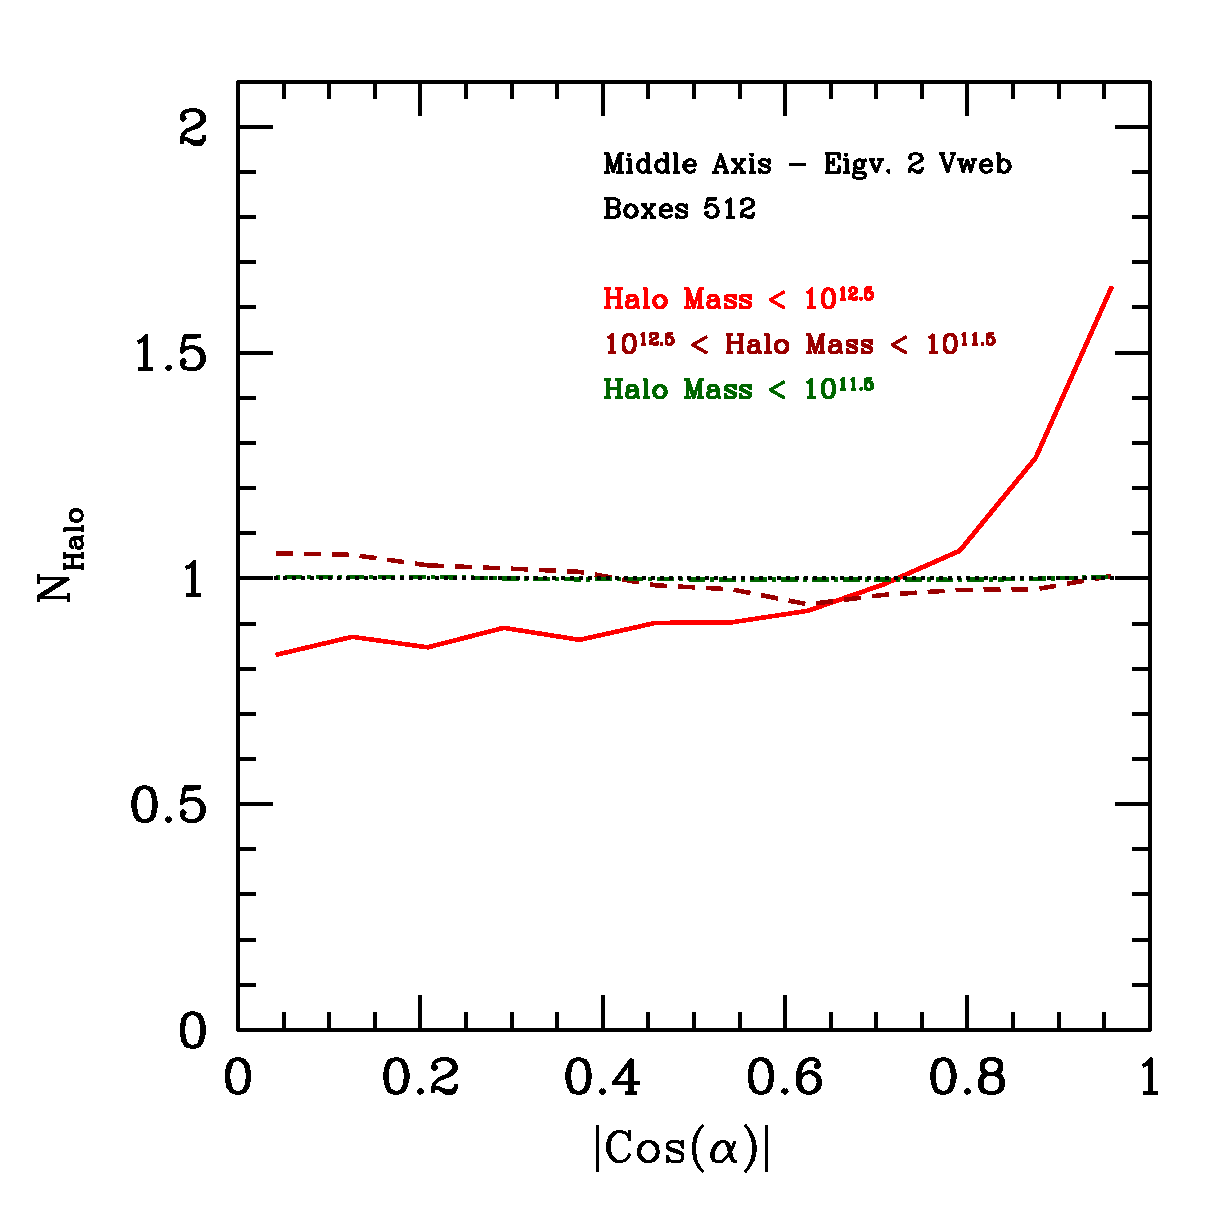
\includegraphics[width=0.30\textwidth]{../plot2/Ax2_VT/512_AX2_V2.ps}
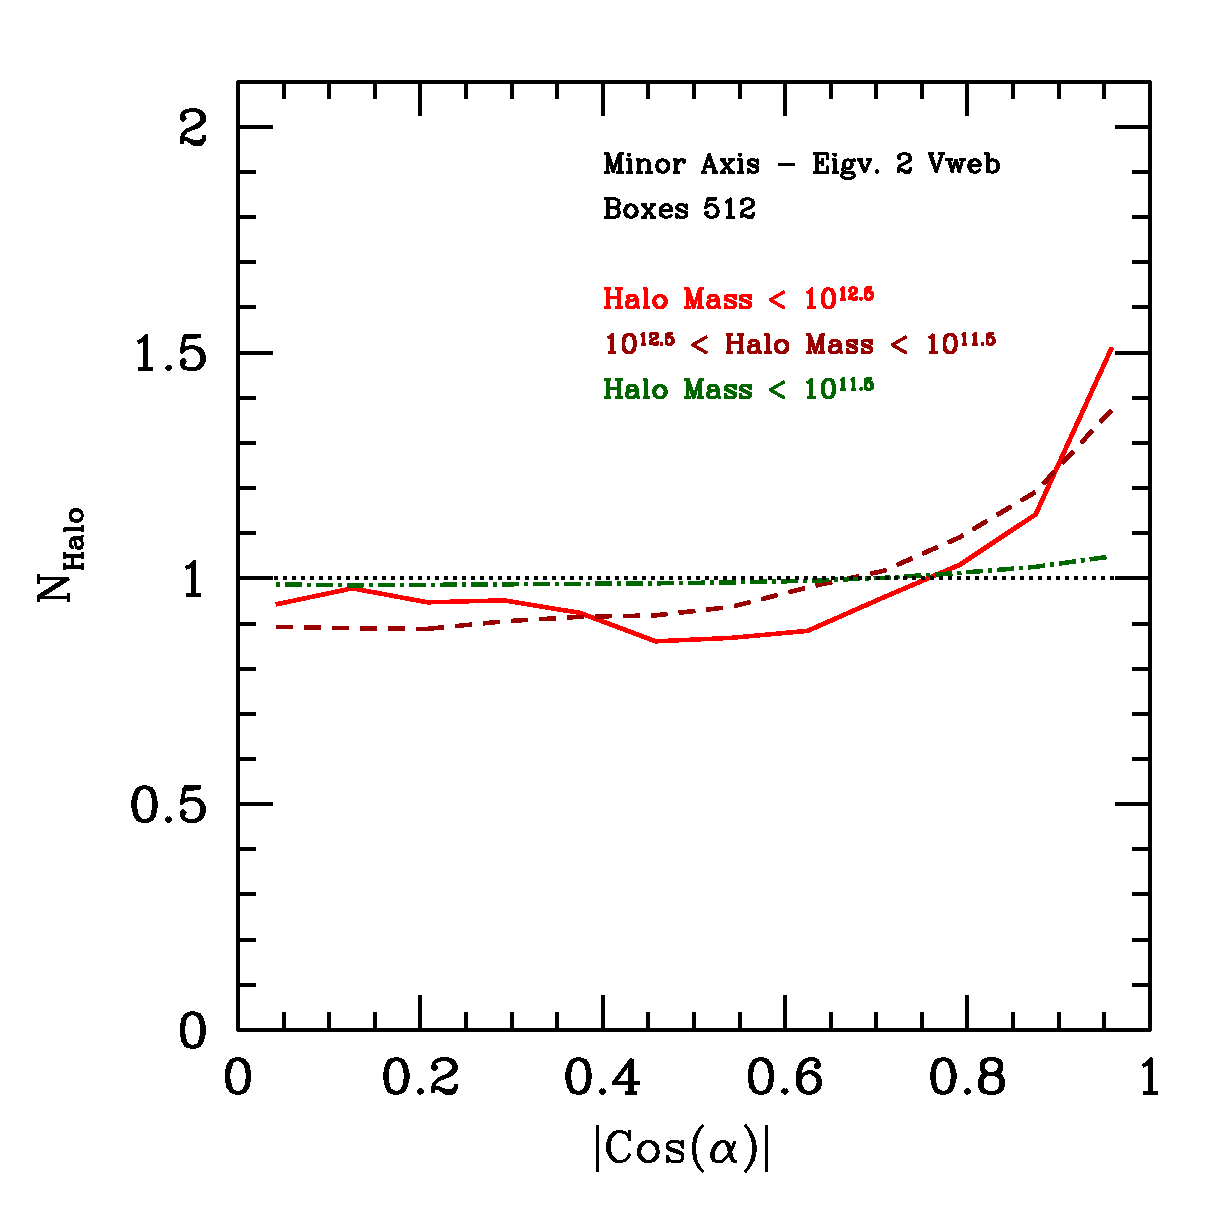
\includegraphics[width=0.30\textwidth]{../plot2/Ax3_VT/512_AX3_V2.ps}
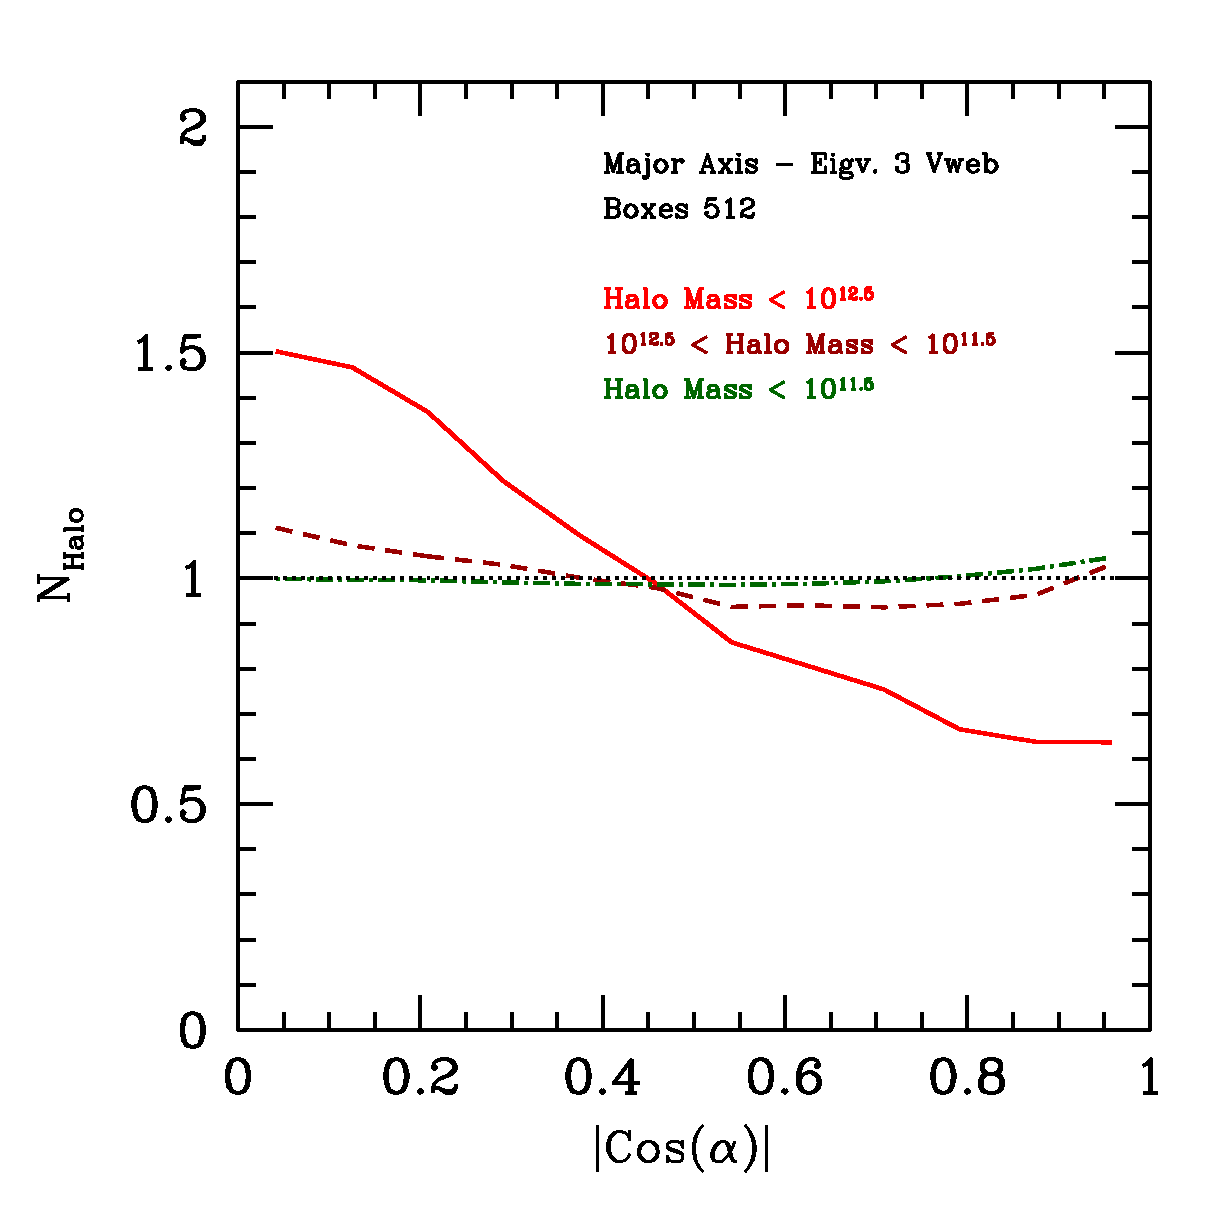
\includegraphics[width=0.30\textwidth]{../plot2/Ax1_VT/512_AX1_V3.ps}
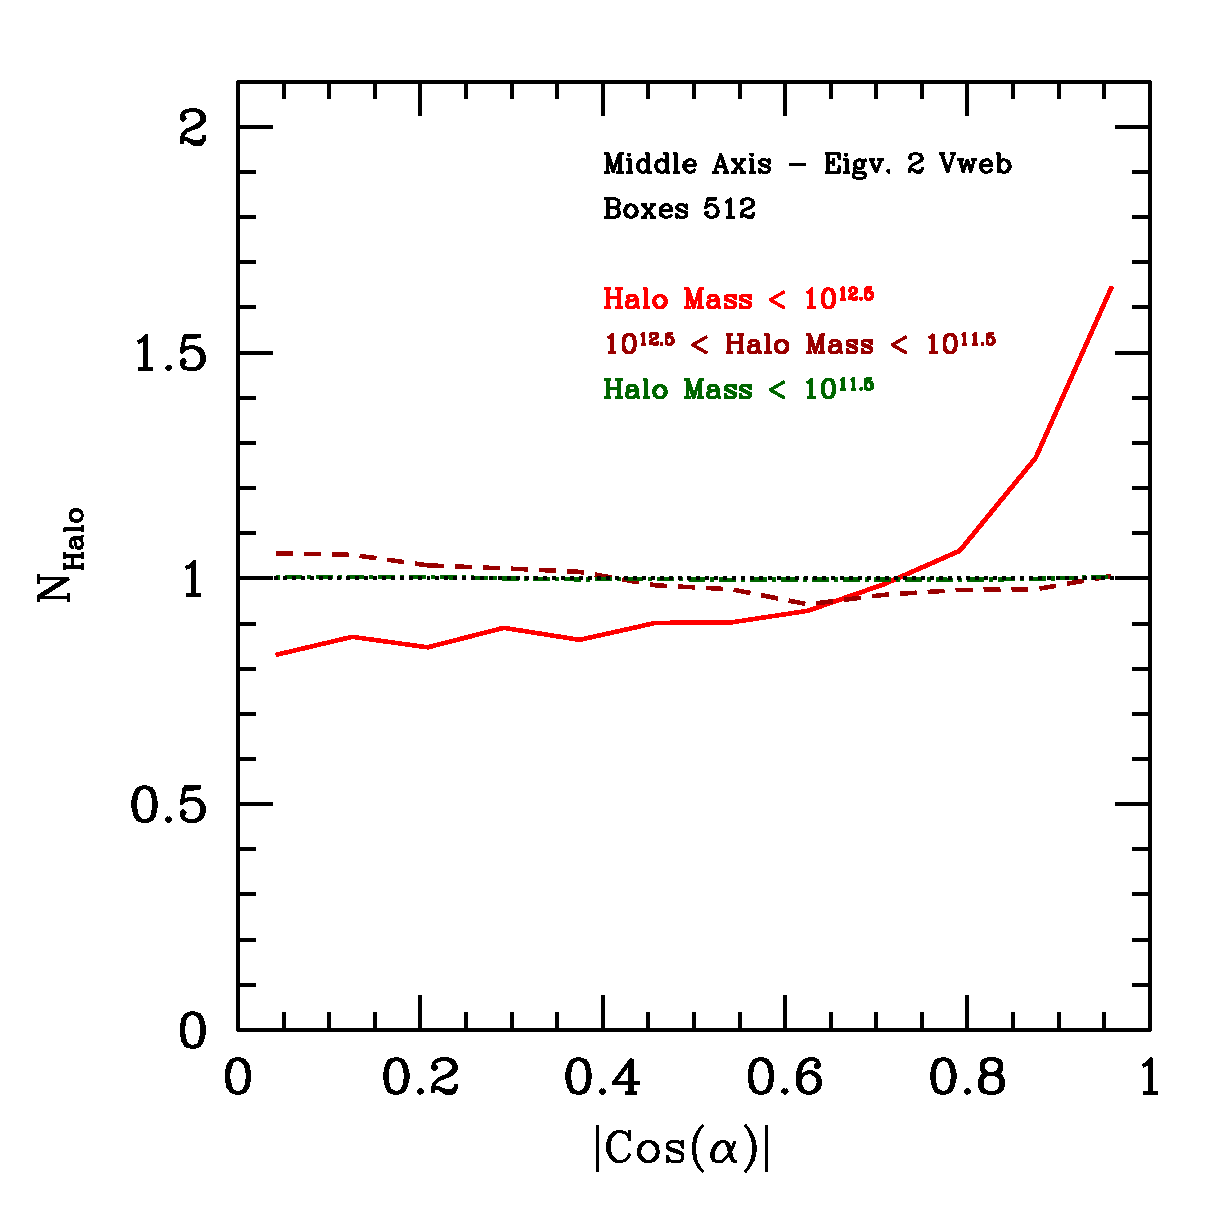
\includegraphics[width=0.30\textwidth]{../plot2/Ax2_VT/512_AX2_V2.ps}
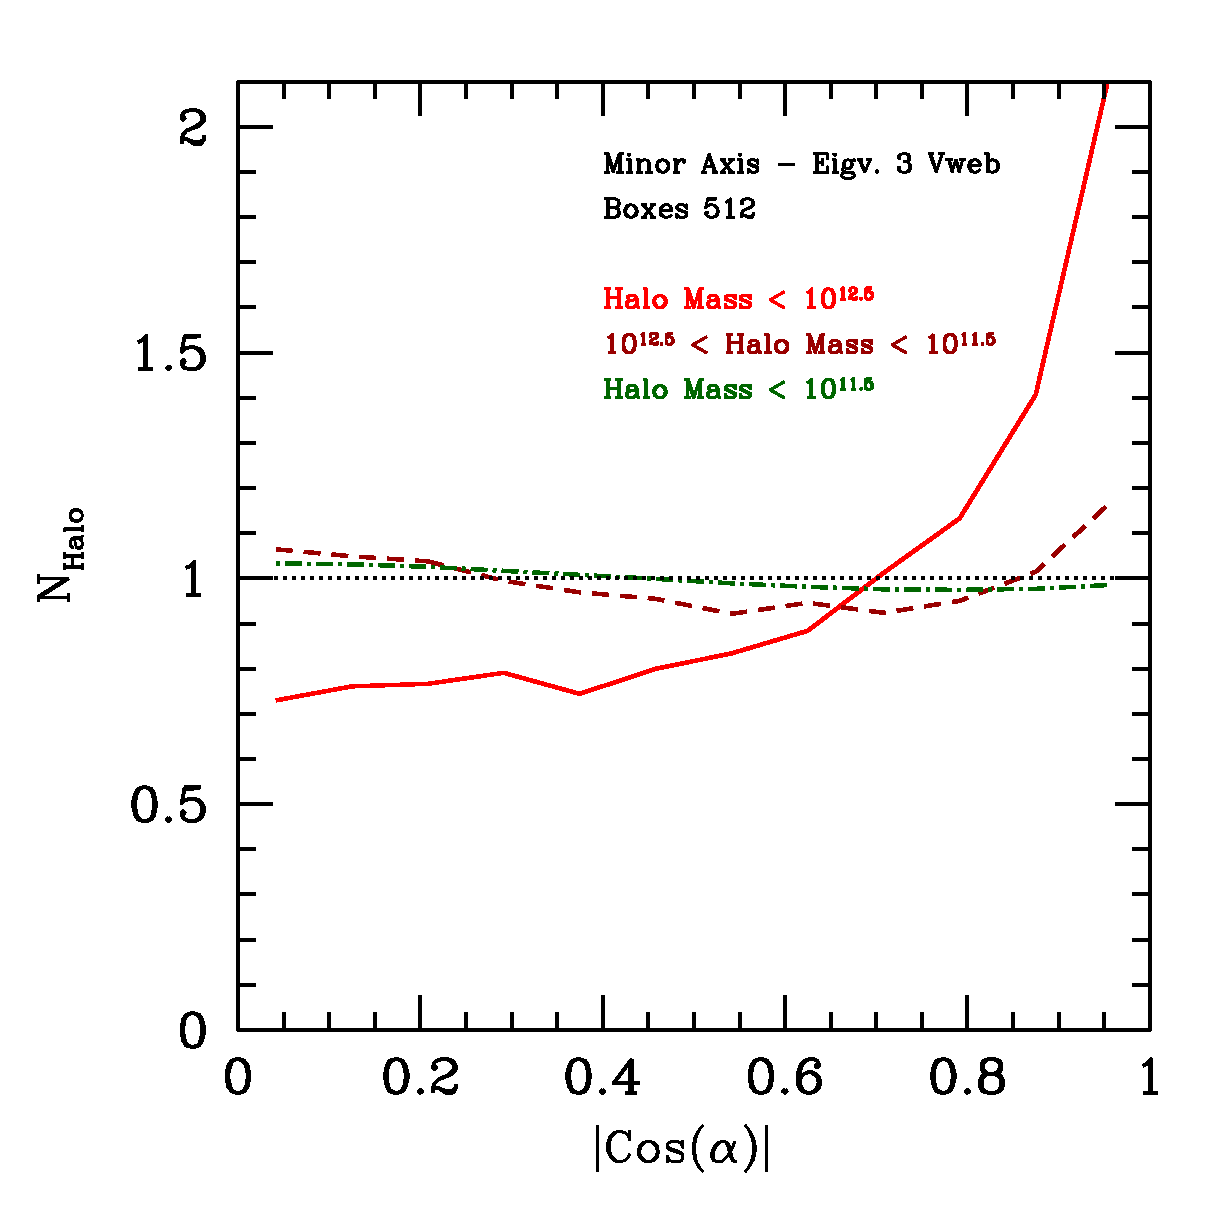
\includegraphics[width=0.30\textwidth]{../plot2/Ax3_VT/512_AX3_V3.ps}
\caption{Shape alignment for the vweb at $512^3$ resolution.}
\end{figure*}

\begin{figure*}
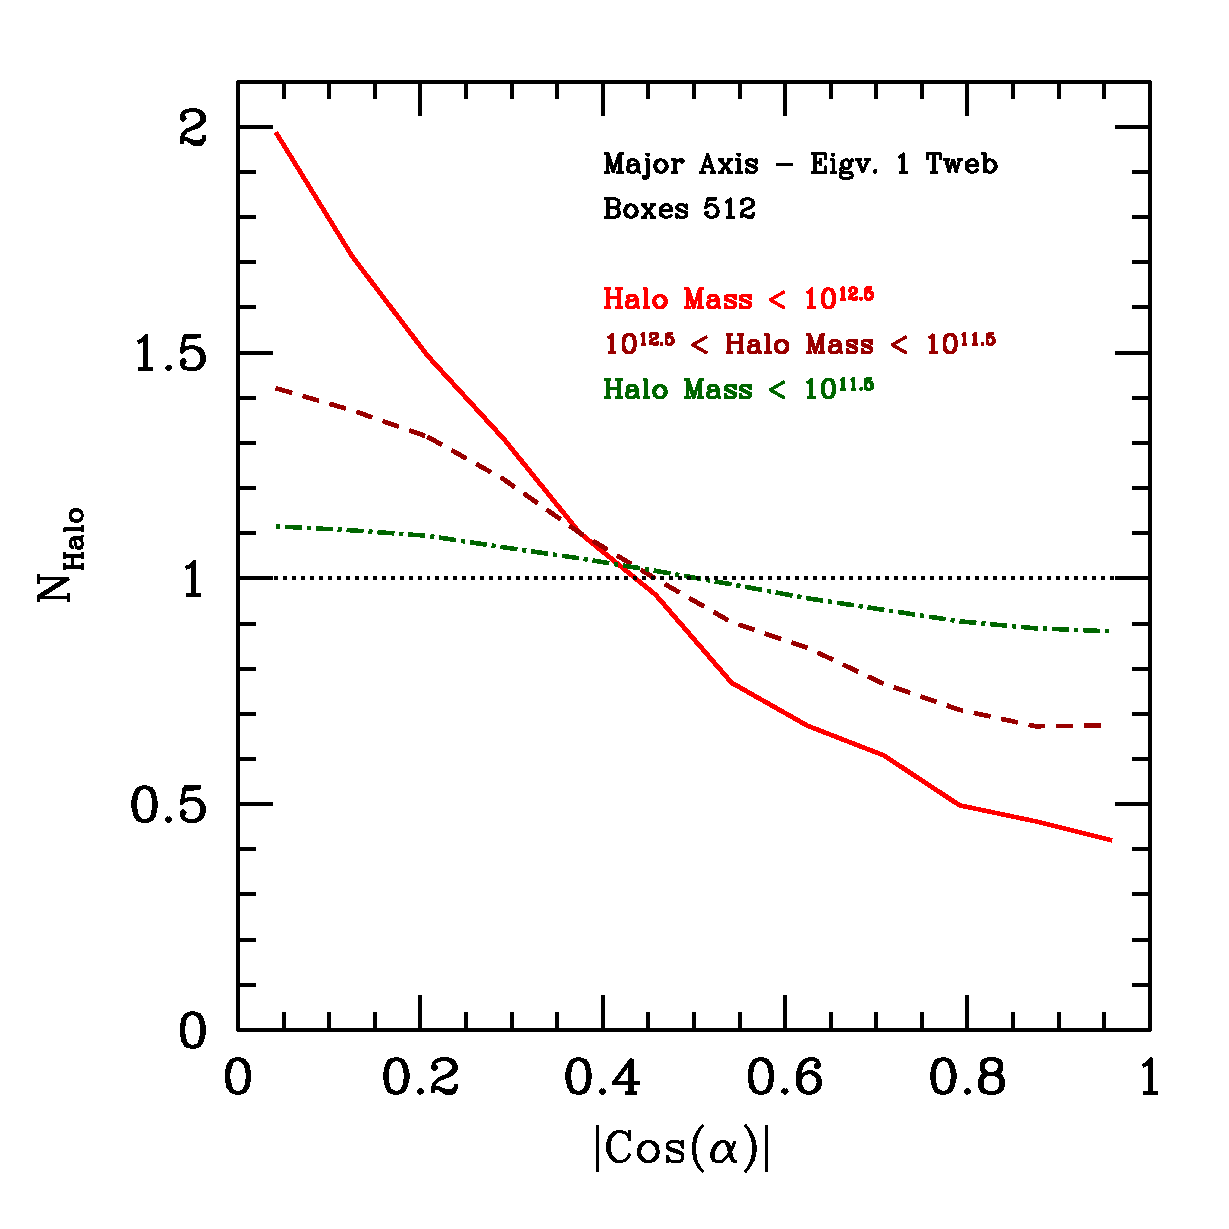
\includegraphics[width=0.30\textwidth]{../plot2/Ax1_VT/512_AX1_T1.ps}
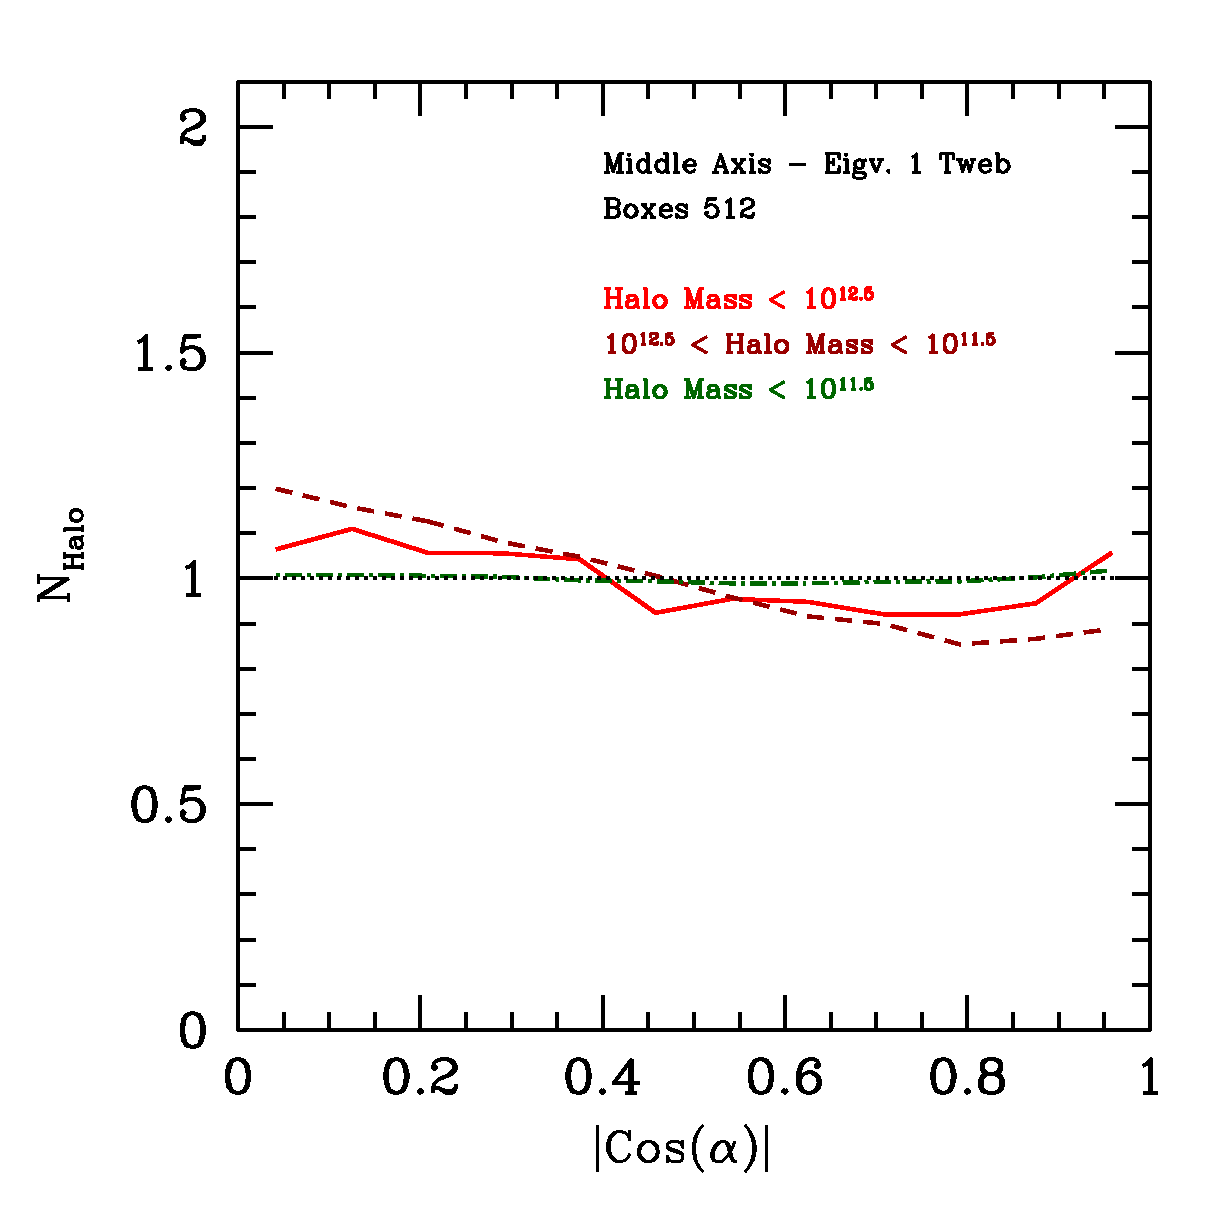
\includegraphics[width=0.30\textwidth]{../plot2/Ax2_VT/512_AX2_T1.ps}
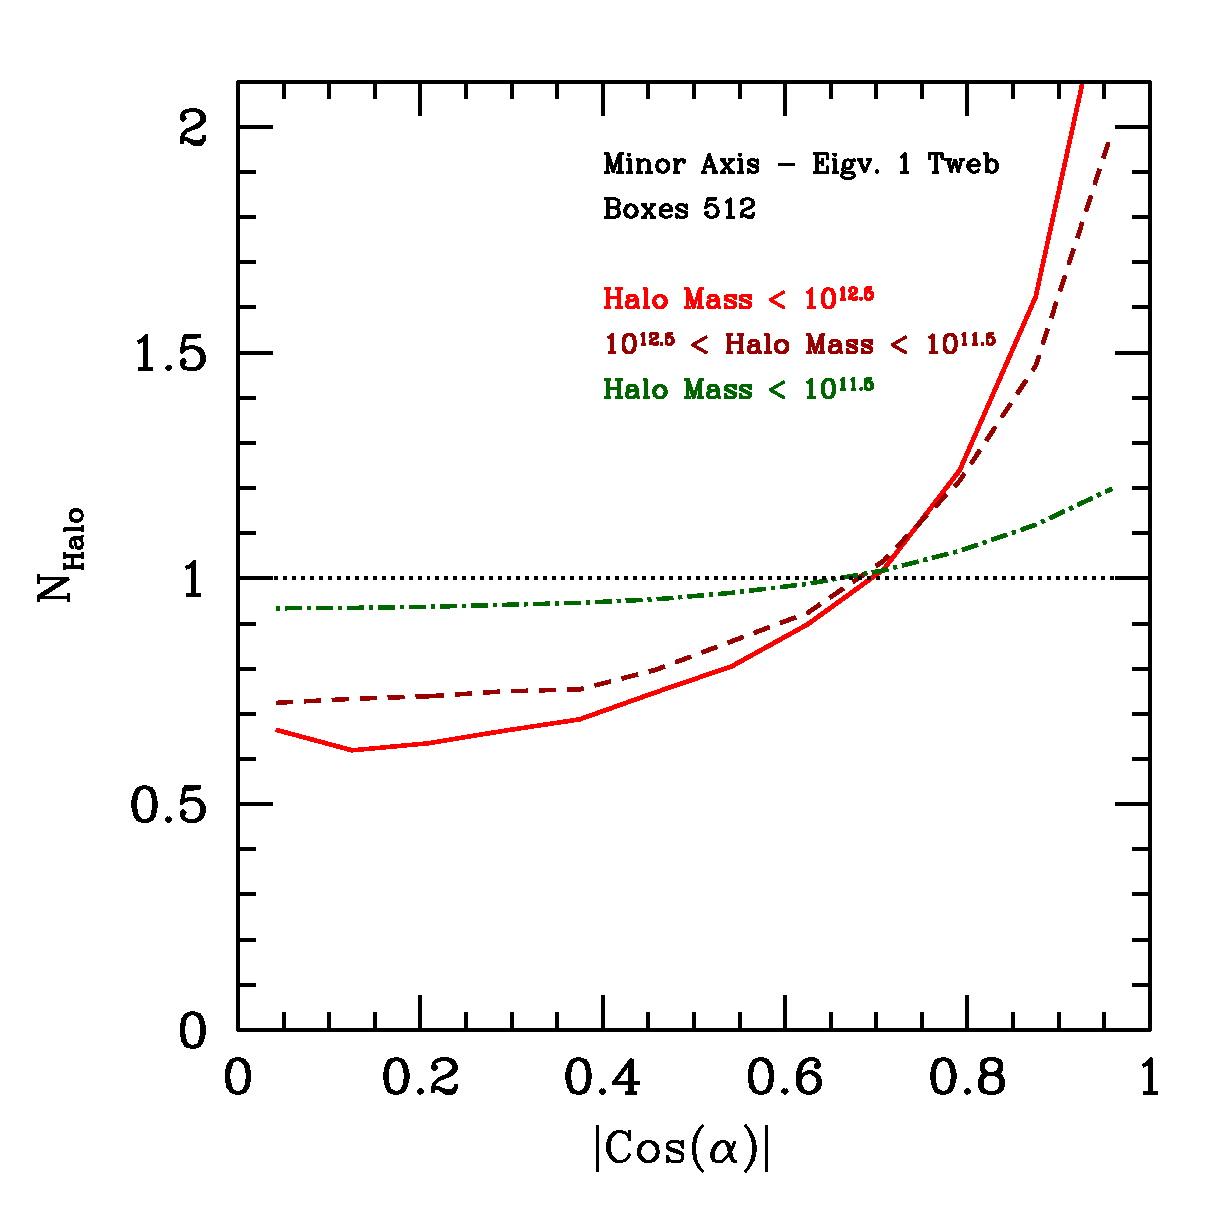
\includegraphics[width=0.30\textwidth]{../plot2/Ax3_VT/512_AX3_T1.ps}
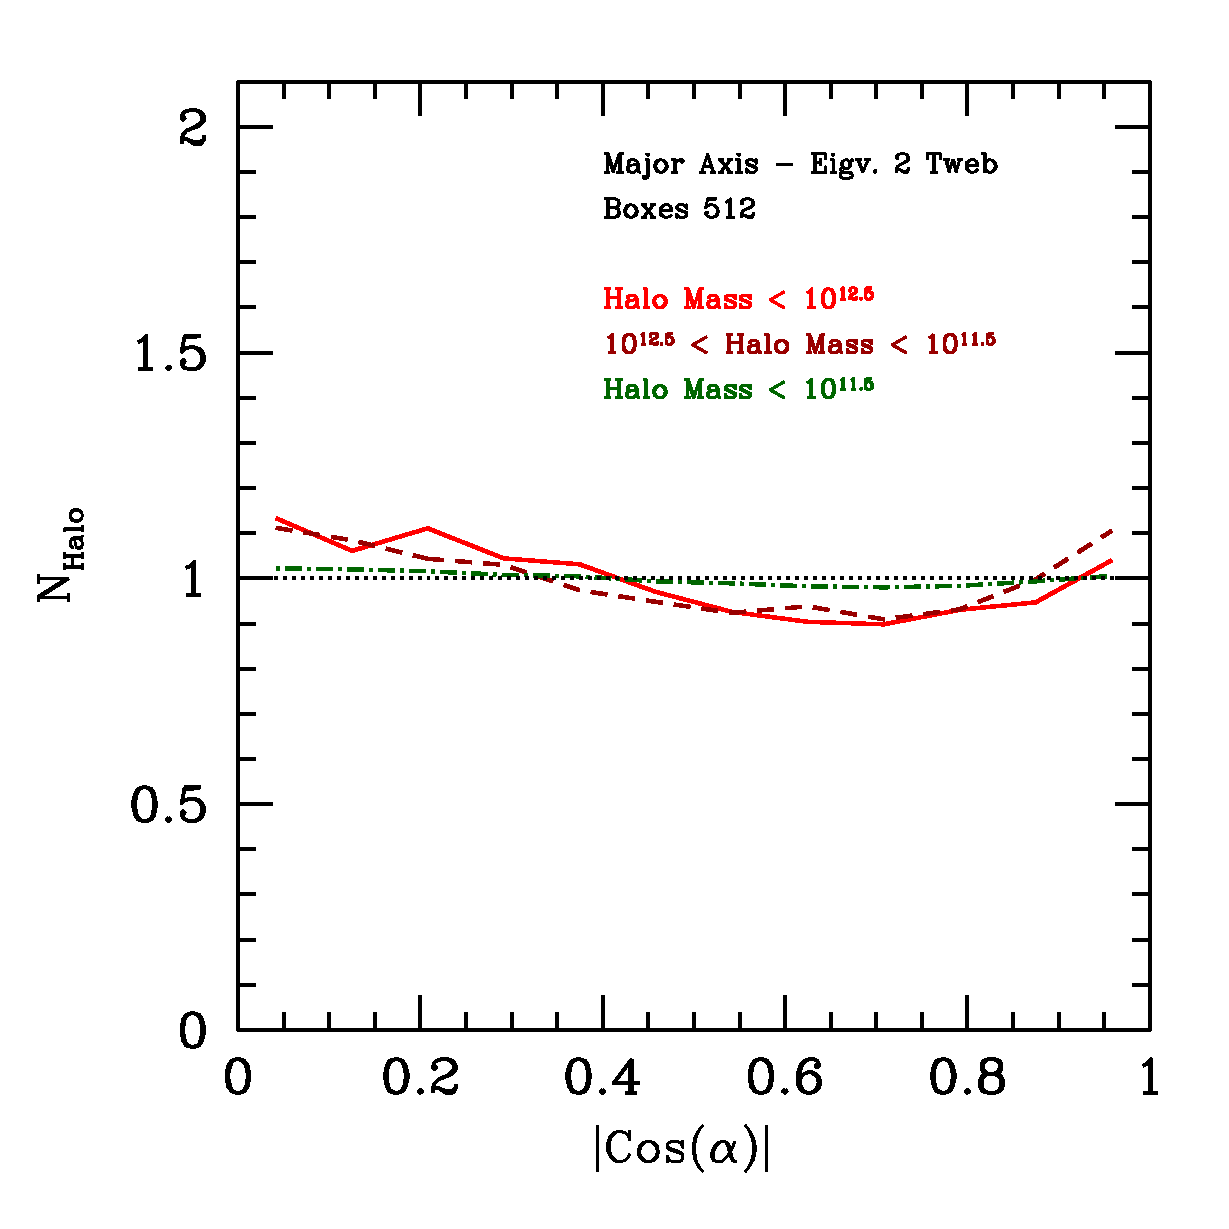
\includegraphics[width=0.30\textwidth]{../plot2/Ax1_VT/512_AX1_T2.ps}
\includegraphics[width=0.30\textwidth]{../plot2/Ax2_VT/512_AX2_T2.ps}
\includegraphics[width=0.30\textwidth]{../plot2/Ax3_VT/512_AX3_T2.ps}
\includegraphics[width=0.30\textwidth]{../plot2/Ax1_VT/512_AX1_T3.ps}
\includegraphics[width=0.30\textwidth]{../plot2/Ax2_VT/512_AX2_T2.ps}
\includegraphics[width=0.30\textwidth]{../plot2/Ax3_VT/512_AX3_T3.ps}
\caption{Shape alignment for the tweb at $512^3$ resolution.}
\end{figure*}

\begin{figure*}
\includegraphics[width=0.30\textwidth]{../plot2/Mass/VWeb.ps}
\includegraphics[width=0.30\textwidth]{../plot2/Mass/TWeb.ps}
\caption{Median of the shape alignment for the two web  and the two grid resolution.}
\end{figure*}


\newpage
\subsection{Angular Momentum Alignment}

\begin{figure*}
\includegraphics[width=0.30\textwidth]{../plot2/J/256_J_V1.ps}
\includegraphics[width=0.30\textwidth]{../plot2/J/256_J_V2.ps}
\includegraphics[width=0.30\textwidth]{../plot2/J/256_J_V3.ps}
\caption{Angular momentum alignment with the Vweb for $256^3$ grid resolution.}
\end{figure*}


\begin{figure*}
\includegraphics[width=0.30\textwidth]{../plot2/J/512_J_V1.ps}
\includegraphics[width=0.30\textwidth]{../plot2/J/512_J_V2.ps}
\includegraphics[width=0.30\textwidth]{../plot2/J/512_J_V3.ps}
\caption{Angular momentum alignment with the Vweb for $512^3$ grid resolution.}
\end{figure*}


\begin{figure*}
\includegraphics[width=0.30\textwidth]{../plot2/J/256_J_T1.ps}
\includegraphics[width=0.30\textwidth]{../plot2/J/256_J_T2.ps}
\includegraphics[width=0.30\textwidth]{../plot2/J/256_J_T3.ps}
\caption{Angular momentum alignment with the Tweb for $256^3$ grid resolution.}
\end{figure*}


\begin{figure*}
\includegraphics[width=0.30\textwidth]{../plot2/J/512_J_T1.ps}
\includegraphics[width=0.30\textwidth]{../plot2/J/512_J_T2.ps}
\includegraphics[width=0.30\textwidth]{../plot2/J/512_J_T3.ps}
\caption{Angular momentum alignment with the Tweb for $512^3$ grid resolution.}
\end{figure*}


\begin{figure*}
\includegraphics[width=0.30\textwidth]{../plot2/Mass/jVWeb.ps}
\includegraphics[width=0.30\textwidth]{../plot2/Mass/jTWeb.ps}
\caption{Median of the angular momentum for the two web  and the two grid resolution.}
\end{figure*}



\subsection{Peculiar velocity Alignment}

\begin{figure*}
\includegraphics[width=0.30\textwidth]{../plot2/Vel/256_vel_V1.ps}
\includegraphics[width=0.30\textwidth]{../plot2/Vel/256_vel_V2.ps}
\includegraphics[width=0.30\textwidth]{../plot2/Vel/256_vel_V3.ps}
\caption{Peculiar velocity alignment with the Vweb for $256^3$ grid resolution.}
\end{figure*}


\begin{figure*}
\includegraphics[width=0.30\textwidth]{../plot2/Vel/512_vel_V1.ps}
\includegraphics[width=0.30\textwidth]{../plot2/Vel/512_vel_V2.ps}
\includegraphics[width=0.30\textwidth]{../plot2/Vel/512_vel_V3.ps}
\caption{Peculiar velocity alignment with the Vweb for $512^3$ grid resolution.}
\end{figure*}


\begin{figure*}
\includegraphics[width=0.30\textwidth]{../plot2/Vel/256_vel_T1.ps}
\includegraphics[width=0.30\textwidth]{../plot2/Vel/256_vel_T2.ps}
\includegraphics[width=0.30\textwidth]{../plot2/Vel/256_vel_T3.ps}
\caption{Peculiar velocity alignment with the Tweb for $256^3$ grid resolution.}
\end{figure*}


%\begin{figure*}
%\includegraphics[width=0.30\textwidth]{../plot2/Vel/512_vel_T1.ps}
%\includegraphics[width=0.30\textwidth]{../plot2/Vel/512_vel_T2.ps}
%\includegraphics[width=0.30\textwidth]{../plot2/Vel/512_vel_T3.ps}
%\caption{Peculiar velocity alignment with the Tweb for $512^3$ grid resolution.}
%\end{figure*}

%\begin{figure*}
%\includegraphics[width=0.30\textwidth]{../plot2/Mass/vVWeb.ps}
%\includegraphics[width=0.30\textwidth]{../plot2/Mass/vTWeb.ps}
%\caption{Median of the peculiar velocity for the two web  and the two grid resolution.}
%\end{figure*}


\begin{figure*}
\includegraphics[width=0.35\textwidth]{../tmp/Type/T_Web_256.ps}
\includegraphics[width=0.35\textwidth]{../tmp/Type/V_Web_256.ps}
\includegraphics[width=0.35\textwidth]{../tmp/Type/JT_Web_256.ps}
\includegraphics[width=0.35\textwidth]{../tmp/Type/JV_Web_256.ps}
\includegraphics[width=0.35\textwidth]{../tmp/Type/vT_Web_256.ps}
\includegraphics[width=0.35\textwidth]{../tmp/Type/vV_Web_256.ps}
\caption{From top to bottom: Shape, J, velocities. 256 resolution. Left Tweb, right Vweb}
\end{figure*}



\begin{figure*}
\includegraphics[width=0.35\textwidth]{../tmp/Type/T_Web_512.ps}
\includegraphics[width=0.35\textwidth]{../tmp/Type/V_Web_512.ps}
\includegraphics[width=0.35\textwidth]{../tmp/Type/JT_Web_512.ps}
\includegraphics[width=0.35\textwidth]{../tmp/Type/JV_Web_512.ps}
\includegraphics[width=0.35\textwidth]{../tmp/Type/vT_Web_512.ps}
\includegraphics[width=0.35\textwidth]{../tmp/Type/vV_Web_512.ps}
\caption{From top to bottom: Shape, J, velocities. 512 resolution. Left Tweb, right Vweb}
\end{figure*}

Possible conclusion. Prolateness follow concentration. In the Tweb Angular momentum alignment is influenced by spin at higher masses. In the Vweb angular momentum alginment is influenced by all factors. In the peculiar velocity alginment only spin seemss to have an effect.

\section{Discussion}
\label{sec:discussion}


\section{Conclusions}
\label{sec:conclusions}


\section*{Acknowledgments} 

\bibliographystyle{mn2e}
\bibliography{references} 



\end{document}
